\documentclass[a4paper]{article}

\def\npart {II}
\def\nterm {Lent}
\def\nyear {2017}
\def\nlecturer {H.\ S.\ Reall}
\def\ncourse {Statistical Physics}

\usepackage{myheader}

\def\di{{\mathchar'26\mkern-12mu d}}
\def\isothermia{(1.6,0.3) (1.7,0.19847) (1.8,0.14429) (1.9,0.11496) (2.0,0.10000) (2.1,0.09349) (2.2,0.09194)}
\def\isothermib{(2.2,0.09194) (2.3,0.09328) (2.4,0.09623) (2.5,0.10000) (2.6,0.10411) (2.7,0.10825) (2.8,0.11224) (2.9,0.11600) (3.0,0.11944) (3.1,0.12257) (3.2,0.12536) (3.3,0.12782) (3.4,0.12997) (3.5,0.13184) (3.6,0.13343) (3.7,0.13477) (3.8,0.13588) (3.9,0.13679) (4.0,0.13750) (4.1,0.13804) (4.2,0.13843) (4.3,0.13867) (4.4,0.13879) (4.5,0.13880)}
\def\isothermic{(4.5,0.13880) (4.6,0.13871) (4.7,0.13852) (4.8,0.13825) (4.9,0.13791) (5.0,0.13750) (5.1,0.13703) (5.2,0.13652) (5.3,0.13595) (5.4,0.13535) (5.5,0.13471) (5.6,0.13404) (5.7,0.13334) (5.8,0.13262) (5.9,0.13187) (6.0,0.13111) (6.1,0.13033) (6.2,0.12954) (6.3,0.12874) (6.4,0.12793) (6.5,0.12711) (6.6,0.12629) (6.7,0.12546) (6.8,0.12463) (6.9,0.12379) (7.0,0.12296) (7.1,0.12212) (7.2,0.12129) (7.3,0.12046) (7.4,0.11963) (7.5,0.11880) (7.6,0.11798) (7.7,0.11716) (7.8,0.11635) (7.9,0.11554) (8.0,0.11473) (8.1,0.11393) (8.2,0.11314) (8.3,0.11235) (8.4,0.11157) (8.5,0.11080) (8.6,0.11003) (8.7,0.10927) (8.8,0.10851) (8.9,0.10776) (9.0,0.10702) (9.1,0.10629) (9.2,0.10556) (9.3,0.10484) (9.4,0.10413) (9.5,0.10342) (9.6,0.10272) (9.7,0.10203) (9.8,0.10135) (9.9,0.10067) (10.0,0.10000) (10.1,0.09934) (10.2,0.09868) (10.3,0.09803) (10.4,0.09739) (10.5,0.09675) (10.6,0.09613) (10.7,0.09550) (10.8,0.09489) (10.9,0.09428) (11.0,0.09368) (11.1,0.09308) (11.2,0.09249) (11.3,0.09191) (11.4,0.09133) (11.5,0.09076) (11.6,0.09020) (11.7,0.08964) (11.8,0.08909) (11.9,0.08854) (12.0,0.08801) (12.1,0.08747) (12.2,0.08694) (12.3,0.08642) (12.4,0.08590) (12.5,0.08539) (12.6,0.08489) (12.7,0.08438) (12.8,0.08389) (12.9,0.08340) (13.0,0.08291) (13.1,0.08243) (13.2,0.08196) (13.3,0.08149) (13.4,0.08103) (13.5,0.08057) (13.6,0.08011) (13.7,0.07966) (13.8,0.07921) (13.9,0.07877) (14.0,0.07834) (14.1,0.07790) (14.2,0.07748) (14.3,0.07705) (14.4,0.07663) (14.5,0.07622) (14.6,0.07581) (14.7,0.07540) (14.8,0.07500) (14.9,0.07460) (15.0,0.07421)}
\def\isothermi{\isothermia \isothermib \isothermic}
\def\isothermii{(1.8,0.3) (1.9,0.26107) (2.0,0.23150) (2.1,0.21303) (2.2,0.20153) (2.3,0.19444) (2.4,0.19016) (2.5,0.18767) (2.6,0.18629) (2.7,0.18560) (2.8,0.18530) (2.9,0.18521) (3.0,0.18519) (3.1,0.18518) (3.2,0.18513) (3.3,0.18499) (3.4,0.18477) (3.5,0.18444) (3.6,0.18401) (3.7,0.18347) (3.8,0.18285) (3.9,0.18213) (4.0,0.18133) (4.1,0.18046) (4.2,0.17952) (4.3,0.17852) (4.4,0.17747) (4.5,0.17637) (4.6,0.17523) (4.7,0.17406) (4.8,0.17285) (4.9,0.17163) (5.0,0.17038) (5.1,0.16911) (5.2,0.16783) (5.3,0.16654) (5.4,0.16524) (5.5,0.16393) (5.6,0.16263) (5.7,0.16132) (5.8,0.16001) (5.9,0.15871) (6.0,0.15741) (6.1,0.15612) (6.2,0.15483) (6.3,0.15355) (6.4,0.15228) (6.5,0.15102) (6.6,0.14977) (6.7,0.14853) (6.8,0.14730) (6.9,0.14608) (7.0,0.14488) (7.1,0.14368) (7.2,0.14250) (7.3,0.14133) (7.4,0.14018) (7.5,0.13903) (7.6,0.13790) (7.7,0.13679) (7.8,0.13568) (7.9,0.13459) (8.0,0.13352) (8.1,0.13245) (8.2,0.13140) (8.3,0.13037) (8.4,0.12934) (8.5,0.12833) (8.6,0.12733) (8.7,0.12634) (8.8,0.12537) (8.9,0.12441) (9.0,0.12346) (9.1,0.12252) (9.2,0.12160) (9.3,0.12068) (9.4,0.11978) (9.5,0.11889) (9.6,0.11801) (9.7,0.11715) (9.8,0.11629) (9.9,0.11545) (10.0,0.11461) (10.1,0.11379) (10.2,0.11297) (10.3,0.11217) (10.4,0.11138) (10.5,0.11060) (10.6,0.10982) (10.7,0.10906) (10.8,0.10831) (10.9,0.10756) (11.0,0.10683) (11.1,0.10610) (11.2,0.10539) (11.3,0.10468) (11.4,0.10398) (11.5,0.10329) (11.6,0.10261) (11.7,0.10193) (11.8,0.10127) (11.9,0.10061) (12.0,0.09996) (12.1,0.09932) (12.2,0.09868) (12.3,0.09806) (12.4,0.09744) (12.5,0.09683) (12.6,0.09622) (12.7,0.09562) (12.8,0.09503) (12.9,0.09445) (13.0,0.09387) (13.1,0.09330) (13.2,0.09274) (13.3,0.09218) (13.4,0.09163) (13.5,0.09109) (13.6,0.09055) (13.7,0.09001) (13.8,0.08949) (13.9,0.08897) (14.0,0.08845) (14.1,0.08794) (14.2,0.08744) (14.3,0.08694) (14.4,0.08645) (14.5,0.08596) (14.6,0.08548) (14.7,0.08500) (14.8,0.08453) (14.9,0.08406) (15.0,0.08360)}
\def\isothermiii{(2.2,0.3) (2.3,0.28559) (2.4,0.27480) (2.5,0.26667) (2.6,0.26036) (2.7,0.25531) (2.8,0.25113) (2.9,0.24757) (3.0,0.24444) (3.1,0.24161) (3.2,0.23899) (3.3,0.23652) (3.4,0.23414) (3.5,0.23184) (3.6,0.22958) (3.7,0.22736) (3.8,0.22517) (3.9,0.22299) (4.0,0.22083) (4.1,0.21869) (4.2,0.21655) (4.3,0.21443) (4.4,0.21232) (4.5,0.21023) (4.6,0.20815) (4.7,0.20609) (4.8,0.20404) (4.9,0.20201) (5.0,0.20000) (5.1,0.19801) (5.2,0.19604) (5.3,0.19409) (5.4,0.19217) (5.5,0.19027) (5.6,0.18839) (5.7,0.18653) (5.8,0.18470) (5.9,0.18289) (6.0,0.18111) (6.1,0.17935) (6.2,0.17762) (6.3,0.17591) (6.4,0.17423) (6.5,0.17257) (6.6,0.17093) (6.7,0.16932) (6.8,0.16773) (6.9,0.16617) (7.0,0.16463) (7.1,0.16311) (7.2,0.16161) (7.3,0.16014) (7.4,0.15869) (7.5,0.15726) (7.6,0.15586) (7.7,0.15447) (7.8,0.15311) (7.9,0.15177) (8.0,0.15045) (8.1,0.14914) (8.2,0.14786) (8.3,0.14660) (8.4,0.14535) (8.5,0.14413) (8.6,0.14292) (8.7,0.14173) (8.8,0.14056) (8.9,0.13941) (9.0,0.13827) (9.1,0.13715) (9.2,0.13605) (9.3,0.13496) (9.4,0.13389) (9.5,0.13283) (9.6,0.13179) (9.7,0.13077) (9.8,0.12976) (9.9,0.12876) (10.0,0.12778) (10.1,0.12681) (10.2,0.12585) (10.3,0.12491) (10.4,0.12398) (10.5,0.12307) (10.6,0.12217) (10.7,0.12128) (10.8,0.12040) (10.9,0.11953) (11.0,0.11868) (11.1,0.11783) (11.2,0.11700) (11.3,0.11618) (11.4,0.11537) (11.5,0.11457) (11.6,0.11379) (11.7,0.11301) (11.8,0.11224) (11.9,0.11148) (12.0,0.11073) (12.1,0.10999) (12.2,0.10926) (12.3,0.10854) (12.4,0.10783) (12.5,0.10713) (12.6,0.10644) (12.7,0.10575) (12.8,0.10508) (12.9,0.10441) (13.0,0.10375) (13.1,0.10310) (13.2,0.10245) (13.3,0.10182) (13.4,0.10119) (13.5,0.10057) (13.6,0.09995) (13.7,0.09934) (13.8,0.09875) (13.9,0.09815) (14.0,0.09757) (14.1,0.09699) (14.2,0.09642) (14.3,0.09585) (14.4,0.09529) (14.5,0.09474) (14.6,0.09419) (14.7,0.09365) (14.8,0.09312) (14.9,0.09259) (15.0,0.09206)}
\def\isothermiv{(1.7,0.3) (1.8,0.21929) (1.9,0.18163) (2.0,0.16000) (2.1,0.14803) (2.2,0.14194) (2.3,0.13944) (2.4,0.13909) (2.5,0.14000) (2.6,0.14161) (2.7,0.14354) (2.8,0.14558) (2.9,0.14757) (3.0,0.14944) (3.1,0.15114) (3.2,0.15263) (3.3,0.15391) (3.4,0.15497) (3.5,0.15584) (3.6,0.15651) (3.7,0.15699) (3.8,0.15731) (3.9,0.15748) (4.0,0.15750) (4.1,0.15740) (4.2,0.15718) (4.3,0.15686) (4.4,0.15644) (4.5,0.15594) (4.6,0.15537) (4.7,0.15473) (4.8,0.15404) (4.9,0.15329) (5.0,0.15250) (5.1,0.15167) (5.2,0.15080) (5.3,0.14991) (5.4,0.14899) (5.5,0.14804) (5.6,0.14708) (5.7,0.14611) (5.8,0.14512) (5.9,0.14412) (6.0,0.14311) (6.1,0.14210) (6.2,0.14108) (6.3,0.14006) (6.4,0.13904) (6.5,0.13802) (6.6,0.13700) (6.7,0.13599) (6.8,0.13497) (6.9,0.13396) (7.0,0.13296) (7.1,0.13196) (7.2,0.13097) (7.3,0.12998) (7.4,0.12900) (7.5,0.12803) (7.6,0.12707) (7.7,0.12612) (7.8,0.12517) (7.9,0.12423) (8.0,0.12330) (8.1,0.12238) (8.2,0.12147) (8.3,0.12057) (8.4,0.11968) (8.5,0.11880) (8.6,0.11792) (8.7,0.11706) (8.8,0.11620) (8.9,0.11536) (9.0,0.11452) (9.1,0.11369) (9.2,0.11288) (9.3,0.11207) (9.4,0.11127) (9.5,0.11048) (9.6,0.10970) (9.7,0.10893) (9.8,0.10817) (9.9,0.10741) (10.0,0.10667) (10.1,0.10593) (10.2,0.10520) (10.3,0.10448) (10.4,0.10377) (10.5,0.10307) (10.6,0.10238) (10.7,0.10169) (10.8,0.10101) (10.9,0.10034) (11.0,0.09968) (11.1,0.09902) (11.2,0.09838) (11.3,0.09774) (11.4,0.09710) (11.5,0.09648) (11.6,0.09586) (11.7,0.09525) (11.8,0.09465) (11.9,0.09405) (12.0,0.09346) (12.1,0.09288) (12.2,0.09230) (12.3,0.09173) (12.4,0.09117) (12.5,0.09061) (12.6,0.09006) (12.7,0.08951) (12.8,0.08897) (12.9,0.08844) (13.0,0.08791) (13.1,0.08739) (13.2,0.08688) (13.3,0.08637) (13.4,0.08586) (13.5,0.08537) (13.6,0.08487) (13.7,0.08438) (13.8,0.08390) (13.9,0.08342) (14.0,0.08295) (14.1,0.08248) (14.2,0.08202) (14.3,0.08156) (14.4,0.08111) (14.5,0.08066) (14.6,0.08022) (14.7,0.07978) (14.8,0.07935) (14.9,0.07892) (15.0,0.07849)}
% map (\x -> (showFFloat (Just 1) x "", showFFloat (Just 5) (1.35 / (x - 1) - 5 / x^2) "")) [1.6,1.7..15]
% map (\x -> (showFFloat (Just 1) x "", showFFloat (Just 5) (1.4815/ (x - 1) - 5 / x^2) "")) [1.8,1.9..15]
% map (\x -> (showFFloat (Just 1) x "", showFFloat (Just 5) (1.6/ (x - 1) - 5 / x^2) "")) [2.2,2.3..15]
% map (\x -> (showFFloat (Just 1) x "", showFFloat (Just 5) (1.6/ (x - 1) - 5 / x^2) "")) [1.7,1.8..15]

\begin{document}
\maketitle
{\small
  \noindent\emph{Part IB Quantum Mechanics and ``Multiparticle Systems'' from Part II Principles of Quantum Mechanics are essential}

  \vspace{10pt}
  \noindent\textbf{Fundamentals of statistical mechanics}\\
  Microcanonical ensemble. Entropy, temperature and pressure. Laws of thermodynamics. Example of paramagnetism. Boltzmann distribution and canonical ensemble. Partition function. Free energy. Specific heats. Chemical Potential. Grand Canonical Ensemble.\hspace*{\fill} [5]

  \vspace{10pt}
  \noindent\textbf{Classical gases}\\
  Density of states and the classical limit. Ideal gas. Maxwell distribution. Equipartition of energy. Diatomic gas. Interacting gases. Virial expansion. Van der Waal's equation of state. Basic kinetic theory.\hspace*{\fill} [3]

  \vspace{10pt}
  \noindent\textbf{Quantum gases}\\
  Density of states. Planck distribution and black body radiation. Debye model of phonons in solids. Bose--Einstein distribution. Ideal Bose gas and Bose--Einstein condensation. Fermi-Dirac distribution. Ideal Fermi gas. Pauli paramagnetism.\hspace*{\fill}[8]

  \vspace{10pt}
  \noindent\textbf{Thermodynamics}\\
  Thermodynamic temperature scale. Heat and work. Carnot cycle. Applications of laws of thermodynamics. Thermodynamic potentials. Maxwell relations.\hspace*{\fill} [4]

  \vspace{10pt}
  \noindent\textbf{Phase transitions}\\
  Liquid-gas transitions. Critical point and critical exponents. Ising model. Mean field theory. First and second order phase transitions. Symmetries and order parameters.\hspace*{\fill} [4]%
}

\tableofcontents
\setcounter{section}{-1}
\section{Introduction}
In all of our previous physics courses, we mostly focused on ``microscopic'' physics. For example, we used the Schr\"odinger equation to describe the mechanics of a single hydrogen atom. We had to do quite a bit of hard work to figure out exactly how it behaved. But what if we wanted to study a much huger system? Let's say we have a box of hydrogen gas, consisting of $\sim 10^{23}$ molecules. If we tried to solve the Schr\"odinger equation for this system, then, even numerically, it is completely intractable.

So how can we understand such a system? Of course, given these $\sim 10^{23}$ molecules, we are not interested in the detailed dynamics of each molecule. We are only interested in some ``macroscopic'' phenomena. For example, we might want to know its pressure and temperature. So what we want to do is to describe the whole system using just a few ``macroscopic'' variables, and still capture the main properties we are interested.

In the first part of the course, we will approach this subject rather ``rigorously''. We will start from some microscopic laws we know about, and use them to deduce properties of the macroscopic system. This turns out to be rather successful, at least if we treat things sufficiently properly. Surprisingly, it even applies to scenarios where it is absolutely not obvious it should apply!

Historically, this was not how statistical physics was first developed. Instead, we only had the ``macroscopic'' properties we tried to understand. Back in the days, we didn't even know things are made up of atoms! We will try to understand statistical phenomena in purely macroscopic and ``wordy'' terms, and it turns out we can reproduce the same predictions as before.

Finally, we will turn our attention to something rather different in nature --- phase transitions. As we all know, water turns from liquid to gas as we raise the temperature. This transition is an example of a \emph{phase transition}. Of course, this is still a ``macroscopic'' phenomena, fitting in line with the theme of the course. It doesn't make sense to talk about a single molecule transitioning from liquid to gas. Interestingly, when we look at many different systems undergoing phase transitions, they seem to all behave ``in the same way'' near the phase transition. We will figure out why. At least, partially.

Statistical physics is important. As we mentioned, we can use this to make macroscopic predictions from microscopic laws. Thus, this allows us to put our microscopic laws to experimental test. It turns out methods of statistical physics have some far-reaching applications elsewhere. It can be used to study black holes, or even biology!

\section{Fundamentals of statistical mechanics}
\subsection{Microcanonical ensemble}
We begin by considering a rather general system. Suppose we have an isolated system containing $N$ particles, where $N$ is a Large Number\textsuperscript{TM}. The canonical example to keep in mind is a box of gas detached from reality.

\begin{defi}[Microstate]\index{microstate}
  The \emph{microstate} of a system is the actual (quantum) state of the system. This gives a complete description of the system.
\end{defi}

As one would expect, the microstate is very complicated and infeasible to describe, especially when we have \emph{many} particles. In statistical physics, we observe that many microstates are indistinguishable macroscopically. Thus, we only take note of some macroscopically interesting quantities, and use these macroscopic quantities to put a probability distribution on the microstates.

More precisely, we let $\{\bket{n}\}$ be a basis of normalized eigenstates, say
\[
  \hat{H}\bket{n} = E_n \bket{n}.
\]
We let $p(n)$ be the probability that the microstate is $\bket{n}$. Note that this probability is \emph{not} the quantum probability we are used to. It is some probability assigned to reflect our ignorance of the system. Given such probabilities, we can define the expectation of an operator in the least imaginative way:
\begin{defi}[Expectation value]\index{expectation value}
  Given a probability distribution $p(n)$ on the states, the expectation value of an operator $\mathcal{O}$ is
  \[
    \bra \mathcal{O}\ket = \sum_n p(n) \brak{n}\mathcal{O}\bket{n}.
  \]
\end{defi}
If one knows about density operators, we can describe the system as a mixed state with density operator
\[
  \rho = \sum_n p(n) \bket{n}\brak{n}.
\]
There is an equivalent way of looking at this. We can consider an \term{ensemble} consisting of $W \gg 1$ independent copies of our system such that $Wp(n)$ many copies are in the microstate $\bket{n}$. Then the expectation is just the average over the ensemble. For most purposes, how we think about this doesn't really matter.

We shall further assume our system is in \term{equilibrium}, i.e.\ the probability distribution $p(n)$ does not change in time. So in particular $\bra O\ket$ is independent of time. Of course, this does not mean the particles stop moving. The particles are still whizzing around. It's just that the statistical distribution does not change. In this course, we will mostly be talking about equilibrium systems. When we get out of equilibrium, things become very complicated.

The idea of statistical physics is that we have some partial knowledge about the system. For example, we might know its total energy. The microstates that are compatible with this partial knowledge are called \emph{accessible}\index{accessible state}. The \term{fundamental assumption of statistical mechanics} is then
\begin{significant}
  An isolated system in equilibrium is equally likely to be in any of the accessible microstates.
\end{significant}
Thus, different probability distributions, or different ensembles, are distinguished by the partial knowledge we know.
\begin{defi}[Microcanonical ensemble]\index{microcanonical ensemble}
  In a \emph{microcanonical ensemble}, we know the energy is between $E$ and $E + \delta E$, where $\delta E$ is the accuracy of our measuring device. The accessible microstates are those with energy $E \leq E_n \leq E + \delta E$. We let $\Omega(E)$ be the number of such states.
\end{defi}
In practice, $\delta E$ is much much larger than the spacing of energy levels, and so $\Omega(E) \gg 1$. A priori, it seems like our theory will depend on what the value of $\delta E$ is, but as we develop the theory, we will see that this doesn't really matter.

It is crucial here that we are working with a quantum system, so the possible states is discrete, and it makes sense to count the number of systems. We need to do more quite a bit work if we want to do this classically.

\begin{eg}
  Suppose we have $N = 10^{23}$ particles, and each particle can occupy two states $\bket{\uparrow}$ and $\bket{\downarrow}$, which have the same energy $\varepsilon$. Then we always have $N\varepsilon$ total energy, and we have
  \[
    \Omega(N\varepsilon) = 2^{10^{23}}.
  \]
  This is a fantastically huge, mind-boggling number. This is the kind of number we are talking about.
\end{eg}

By the fundamental assumption, we can write
\[
  p(n) =
  \begin{cases}
    \frac{1}{\Omega(E)} & \text{if } E \leq E_n \leq E + \delta E\\
    0 & \text{otherwise}
  \end{cases}.
\]
This is the characteristic distribution of the microcanonical ensemble.

It turns out it is not very convenient to work with $\Omega(E)$. In particular, $\Omega(E)$ is not linear in $N$, the number of particles. Instead, it scales as an exponential of $N$. So we take the logarithm.

\begin{defi}[Boltzmann entropy]\index{Boltzmann entropy}\index{entropy}
  The \emph{(Boltzmann) entropy} is defined as
  \[
    S(E) = k \log \Omega(E),
  \]
  where $k = \SI{1.381e-23}{\joule\per\kelvin}$ is \term{Boltzmann's constant}\index{$k$}.
\end{defi}
This annoying constant $k$ is necessary because when people started doing thermodynamics, they didn't know about statistical physics, and picked weird conventions.

We wrote our expressions as $S(E)$, instead of $S(E, \delta E)$. As promised, the value of $\delta E$ doesn't really matter. We know that $\Omega(E)$ will scale approximately linearly with $\delta E$. So if we, say, double $\delta E$, then $S(E)$ will increase by $k \log 2$, which is incredibly tiny compared to $S(E) = k \log \Omega(E)$. So it doesn't matter which value of $\delta E$ we pick.

Even if you are not so convinced that multiplying $10^{10^{23}}$ by a factor of $2$ or adding $\log 2$ to $10^{23}$ do not really matter, you should be reassured that at the end, we will rarely talk about $\Omega(E)$ or $S(E)$ itself. Instead, we will often divide two different $\Omega$'s to get probabilities, or differentiate $S$ to get other interesting quantities. In these cases, the factors really do not matter.


The second nice property of the entropy is that it is additive --- if we have two \emph{non-interacting} systems with energies $E_{(1)}, E_{(2)}$. Then the total number of states of the combined system is
\[
  \Omega(E_{(1)}, E_{(2)}) = \Omega_{1}(E_{(1)})\Omega_{2} (E_{(2)}).
\]
So when we take the logarithm, we find
\[
  S(E_{(1)}, E_{(2)}) = S(E_{(1)}) + S(E_{(2)}).
\]
Of course, this is not very interesting, until we bring our systems together and let them interact with each other.

\subsubsection*{Interacting systems}
Suppose we bring the two systems together, and let them exchange energy. Then the energy of the individual systems is no longer fixed, and only the total energy
\[
  E_{\mathrm{total}} = E_{(1)} + E_{(2)}
\]
is fixed. Then we find that
\[
  \Omega(E_{\mathrm{total}}) = \sum_{E_i} \Omega_1(E_i) \Omega_2(E_{\mathrm{total}} - E_i),
\]
where we sum over all possible energy levels of the first system. In terms of the entropy of the system, we have
\[
  \Omega(E_{\mathrm{total}}) = \sum_{E_i} \exp\left(\frac{S_1(E_i)}{k} + \frac{S_2(E_{\mathrm{total}} - E_i)}{k}\right)
\]
We can be a bit more precise with what the sum means. We are not summing over all eigenstates. Recall that we have previously fixed an accuracy $\delta E$. So we can imagine dividing the whole energy spectrum into chunks of size $\delta E$, and here we are summing over the chunks.

We know that $S_{1, 2}/k \sim N_{1, 2} \sim 10^{23}$, which is a ridiculously large number. So the sum is overwhelmingly dominated by the term with the largest exponent. Suppose this is maximized when $E_i = E_*$. Then we have
\[
  S(E_{\mathrm{total}}) = k \log \Omega(E_{\mathrm{total}}) \approx S_1(E_*) + S_2(E_{\mathrm{total}} - E_*).
\]
Again, we are not claiming that only the factor coming from $E_*$ has significant contribution. Maybe one or two energy levels next to $E_*$ are also very significant, but taking these into account will only multiply $\Omega(E_{\mathrm{total}})$ by a (relatively) small constant, hence contributes a small additive factor to $S(E_{\mathrm{total}})$, which can be neglected.

Now given any $E_{(1)}$, what is the probability that the actual energy of the first system is $E_{(1)}$? For convenience, we write $E_{(2)} = E_{\mathrm{total}} - E_{(1)}$, the energy of the second system. Then the probability desired is
\[
  \frac{\Omega_1(E_{(1)})\Omega_2(E_{(2)})}{\Omega(E_{\mathrm{total}})} = \exp\left(\frac{1}{k}\left(S_1(E_{(1)}) + S_2(E_{(2)}) - S(E_{\mathrm{total}})\right)\right).
\]
Again recall that the numbers at stake are unimaginably huge. So if $S_1(E_{(1)}) + S_2(E_{(2)})$ is even slightly different from $S(E_{\mathrm{total}})$, then the probability is effectively zero. And by above, for the two quantities to be close, we need $E_{(1)} = E_*$. So for all practical purposes, the value of $E_{(1)}$ is fixed into $E_*$.

Now imagine we prepare two systems separately with energies $E_{(1)}$ and $E_{(2)}$ such that $E_{(1)} \not= E_*$, and then bring the system together, then we are no longer in equilibrium. $E_{(1)}$ will change until it takes value $E_*$, and then entropy of the system will increase from $S_1(E_{(1)}) + S_2(E_{(2)})$ to $S_1(E_*) + S_2(E_{\mathrm{total}} - E_*)$. In particular, the entropy increases.
\begin{law}[Second law of thermodynamics]\index{second law of thermodynamics}
  The entropy of an isolated system increases (or remains the same) in any physical process. In equilibrium, the entropy attains its maximum value.
\end{law}
This prediction is verified by virtually all observations of physics.

While our derivation did not show it is \emph{impossible} to violate the second law of thermodynamics, it is very very very very very very very very unlikely to be violated.

\subsubsection*{Temperature}
Having defined entropy, the next interesting thing we can define is the \emph{temperature}. We assume that $S$ is a smooth function in $E$. Then we can define the temperature as follows:
\begin{defi}[Temperature]\index{temperature}
  The \emph{temperature} is defined to be
  \[
    \frac{1}{T} = \frac{\d S}{\d E}.
  \]
\end{defi}
Why do we call this the temperature? Over the course, we will see that this quantity we decide to call ``temperature'' does behave as we would expect temperature to behave. It is difficult to give further justification of this definition, because even though we vaguely have some idea what temperature is like in daily life, those ideas are very far from anything we can concretely write down or even describe.

One reassuring property we can prove is the following:
\begin{prop}
  Two interacting systems in equilibrium have the same temperature.
\end{prop}

\begin{proof}
  Recall that the equilibrium energy $E_*$ is found by maximizing
  \[
    S_1(E_i) + S_2(E_{\mathrm{total}} - E_i)
  \]
  over all possible $E_i$. Thus, at an equilibrium, the derivative of this expression has to vanish, and the derivative is exactly
  \[
    \left.\frac{\d S_1}{\d E}\right|_{E_{(1)} = E_*} - \left.\frac{\d S_i}{\d E} \right|_{E_{(2)} = E_{\mathrm{total}} - E_*} = 0
  \]
  So we need
  \[
    \frac{1}{T_1} = \frac{1}{T_2}.
  \]
  In other words, we need
  \[
    T_1 = T_2.\qedhere
  \]
\end{proof}

Now suppose initially, our systems have different temperature. We would expect energy to flow from the hotter system to the cooler system. This is indeed the case.

\begin{prop}
  Suppose two systems with initial energies $E_{(1)}, E_{(2)}$ and temperatures $T_1, T_2$ are put into contact. If $T_1 > T_2$, then energy will flow form the first system to the second.
\end{prop}

\begin{proof}
  Since we are not in equilibrium, there must be some energy transfer from one system to the other. Suppose after time $\delta t$, the energy changes by
  \begin{align*}
    E_{(1)} & \mapsto E_{(1)} + \delta E\\
    E_{(2)} & \mapsto E_{(2)} - \delta E,
  \end{align*}
  keeping the total energy constant. Then the change in entropy is given by
  \[
    \delta S = \frac{\d S_1}{\d E} \delta E_{(1)} + \frac{\d S_2}{\d E} \delta E_{(2)} = \left(\frac{1}{T_1} - \frac{1}{T_2}\right) \delta E.
  \]
  By assumption, we know
  \[
    \frac{1}{T_1} - \frac{1}{T_2} < 0,
  \]
  but by the second law of thermodynamics, we know $\delta S$ must increase. So we must have $\delta E < 0$, i.e.\ energy flows from the first system to the second.
\end{proof}
So this notion of temperature agrees with the basic properties of temperature we expect.

Note that these properties we've derived only depends on the fact that $\frac{1}{T}$ is a monotonically decreasing function of $T$. In principle, we could have picked \emph{any} monotonically decreasing function of $T$, and set it to $\frac{\d S}{\d E}$. We will later see that this definition will agree with the other definitions of temperature we have previously seen, e.g.\ via the ideal gas law, and so this is indeed the ``right'' one.

\subsubsection*{Heat capacity}
As we will keep on doing later, we can take different derivatives to get different interesting quantities. This time, we are going to get heat capacity. Recall that $T$ was a function of energy, $T = T(E)$. We will assume that we can invert this function, at least locally, to get $E$ as a function of $T$.
\begin{defi}[Heat capacity]\index{heat capacity}
  The \emph{heat capacity} of a system is
  \[
    C = \frac{\d E}{\d T}.
  \]
  The \term{specific heat capacity} is
  \[
    \frac{C}{\text{mass of system}}.
  \]
\end{defi}
The specific heat capacity is a property of the substance that makes up the system, and not how much stuff there is, as both $C$ and the mass scale linearly with the size of the system.

This is some quantity we can actually physically measure. We can measure the temperature with a thermometer, and it is usually not too difficult to see how much energy we are pumping into a system. Then by measuring the temperature change, we can figure out the heat capacity.

In doing so, we can indirectly measure the entropy, or at least the changes in entropy. Note that we have
\[
  \frac{\d S}{\d T} = \frac{\d S}{\d E} \frac{\d E}{\d T} = \frac{C}{T}.
\]
Integrating up, if the temperature changes from $T_1$ to $T_2$, we know
\[
  \Delta S = \int_{T_1}^{T_2} \frac{C(T)}{T}\;\d T.
\]
As promised, by measuring heat capacity experimentally, we can measure the change in entropy.

The heat capacity is useful in other ways. Recall that to find the equilibrium energy $E_*$, a necessary condition was that it satisfies
\[
  \frac{\d S_1}{\d E} - \frac{\d S_2}{\d E} = 0.
\]
However, we only know that the solution is an extrema, and not necessarily maximum. To figure out if it is the maximum, we take the second derivative. Note that for a single system, we have
\[
  \frac{\d^2 S}{\d E^2} = \frac{\d}{\d E} \left(\frac{1}{T}\right) = -\frac{1}{T^2 C}.
\]
Applying this to two systems, one can check that entropy is maximized at $E_{(1)} = E_*$ if $C_1, C_2 > 0$. The actual computations is left as an exercise on the first example sheet.

Let's look at some actual systems and try to calculate these quantities.
\begin{eg}
  Consider a $2$-state system, where we have $N$ non-interacting particles with fixed positions. Each particle is either in $\bket{\uparrow}$ or $\bket{\downarrow}$. We can think of these as spins, for example. These two states have different energies
  \[
    E_{\uparrow} = \varepsilon,\quad E_{\downarrow} = 0.
  \]
  We let $N_{\uparrow}$ and $N_{\downarrow}$ be the number of particles in $\bket{\uparrow}$ and $\bket{\downarrow}$ respectively. Then the total energy of the system is
  \[
    E = \varepsilon N_{\uparrow}.
  \]
  We want to calculate this quantity $\Omega(E)$. Here in this very contrived example, it is convenient to pick $\delta E < \varepsilon$, so that $\Omega(E)$ is just the number of ways of choosing $N_{\uparrow}$ particles from $N$. By basic combinatorics, we have
  \[
    \Omega(E) = \frac{N!}{N_{\uparrow}! (N - N_\uparrow)!},
  \]
  and
  \[
    S(E) = k \log \left(\frac{N!}{N_{\uparrow}! (N - N_\uparrow)!}\right).
  \]
  This is not an incredibly useful formula. Since we assumed that $N$ and $N_\uparrow$ are huge, we can use \term{Stirling's approximation}
  \[
    N! = \sqrt{2\pi N} N^N e^{-N} \left(1 + O\left(\frac{1}{N}\right)\right).
  \]
  Then we have
  \[
    \log N! = N \log N - N + \frac{1}{2}\log (2\pi N) + O\left(\frac{1}{N}\right).
  \]
  We just use the approximation three times to get
  \begin{align*}
    S(E) &= k\left(N \log N - N - N_\uparrow \log N_\uparrow + N_\uparrow - (N - N_\uparrow) \log(N - N_\uparrow) + N - N_\uparrow\right)\\
    &= -k \left((N - N_\uparrow) \log \left(\frac{N - N_\uparrow}{N}\right) + N_\uparrow \log\left(\frac{N_{\uparrow}}{N}\right)\right)\\
    &= -kN\left(\left(1 - \frac{E}{N\varepsilon}\right) \log\left(1 - \frac{E}{N\varepsilon}\right) + \frac{E}{N\varepsilon} \log\left(\frac{E}{N\varepsilon}\right)\right).
  \end{align*}
  This is better, but we can get much more out of it if we plot it:
  \begin{center}
    \begin{tikzpicture}
      \draw [->] (0, 0) -- (6, 0) node [right] {$E$};
      \draw [->] (0, 0) -- (0, 4) node [above] {$S(E)$};

      \draw [mblue, thick, domain=0.001:4.999] plot [smooth] (\x, {(-4.5) * ((1 - \x/5) * ln (1 - \x/5) + (\x / 5) * ln (\x / 5))});

      \node [left] at (0, 0) {$0$};
      \node [below] at (5, 0) {$N\varepsilon$};
      \node [below] at (2.5, 0) {$N\varepsilon/2$};
      \draw [dashed] (2.5, 0) -- (2.5, 3);

      \draw [dashed] (2.5, 3.119) -- (0, 3.119) node [left] {$Nk \log 2$};
    \end{tikzpicture}
  \end{center}
  The temperature is
  \[
    \frac{1}{T} = \frac{\d S}{\d T} = \frac{k}{\varepsilon} \log \left(\frac{N \varepsilon}{E} - 1\right),
  \]
  and we can invert to get
  \[
    \frac{N_{\uparrow}}{N} = \frac{E}{N\varepsilon} = \frac{1}{e^{\varepsilon /kT} + 1}.
  \]
  Suppose we get to control the temperature of the system, e.g.\ if we put it with a heat reservoir. What happens as we vary our temperature?
  \begin{itemize}
    \item As $T \to 0$, we have $N_\uparrow \to 0$. So the states all try to go to the ground state.
    \item As $T \to \infty$, we find $N_\uparrow/N \to \frac{1}{2}$, and $E \to N\varepsilon/2$.
  \end{itemize}
  The second result is a bit weird. As $T \to \infty$, we might expect all things to go the maximum energy level, and not just half of them.

  To confuse ourselves further, we can plot another graph, for $\frac{1}{T}$ vs $E$. The graph looks like
  \begin{center}
    \begin{tikzpicture}
      \draw [->] (0, 0) -- (6, 0) node [right] {$E$};
      \draw [->] (0, -2.5) -- (0, 2.5) node [above] {$\frac{1}{T}$};

      \draw [mblue, thick, domain=0.1:4.9] plot [smooth] (\x, {(-0.6) * (ln (\x) - ln (5 - \x))});

      \node [left] at (0, 0) {$0$};
      \node [below] at (5, 0) {$N\varepsilon$};
      \node [below] at (2.5, 0) {$N\varepsilon/2$};

    \end{tikzpicture}
  \end{center}
  We see that having energy $> N\varepsilon/2$ corresponds to negative temperature, and to go from positive temperature to negative temperature, we need to pass through infinite temperature. So in some sense, negative temperature is ``hotter'' than infinite temperature.

  What is going on? By definition, negative $T$ means $\Omega(E)$ is a decreasing function of energy. This is a very unusual situation. In this system, all the particles are fixed, and have no kinetic energy. Consequently, the possible energy levels are bounded. If we included kinetic energy into the system, then kinetic energy can be arbitrarily large. In this case, $\Omega(E)$ is usually an increasing function of $E$.

  Negative $T$ has indeed been observed experimentally. This requires setups where the kinetic energy is not so important in the range of energies we are talking about. One particular scenario where this is observed is in nuclear spins of crystals in magnetic fields. If we have a magnetic field, then naturally, most of the spins will align with the field. We now suddenly flip the field, and then most of the spins are anti-aligned, and this can give us a negative temperature state.

  Now we can't measure negative temperature by sticking a thermometer into the material and getting a negative answer. Something that \emph{can} be interestingly measured is the heat capacity
  \[
    C = \frac{\d E}{\d T} = \frac{N\varepsilon^2}{ kT^2 } \frac{e^{\varepsilon/kT}}{(e^{\varepsilon/kT} + 1)^2}.
  \]
  This again exhibits some peculiar properties. We begin by looking at a plot:
  \begin{center}
    \begin{tikzpicture}[xscale=1.5]
      \draw [->] (0, 0) -- (4, 0) node [right] {$T$};
      \draw [->] (0, 0) -- (0, 4) node [above] {$C$};

      \draw [mblue, thick ] plot coordinates {(0.01,0.00000) (0.04,0.00000) (0.07,0.00102) (0.10,0.03632) (0.13,0.21581) (0.16,0.60094) (0.19,1.13589) (0.22,1.71794) (0.25,2.26083) (0.28,2.71418) (0.31,3.05901) (0.34,3.29686) (0.37,3.44009) (0.40,3.50519) (0.43,3.50895) (0.46,3.46653) (0.49,3.39067) (0.52,3.29165) (0.55,3.17751) (0.58,3.05435) (0.61,2.92675) (0.64,2.79804) (0.67,2.67060) (0.70,2.54609) (0.73,2.42564) (0.76,2.30996) (0.79,2.19945) (0.82,2.09433) (0.85,1.99462) (0.88,1.90026) (0.91,1.81111) (0.94,1.72699) (0.97,1.64766) (1.00,1.57290) (1.03,1.50244) (1.06,1.43606) (1.09,1.37350) (1.12,1.31453) (1.15,1.25893) (1.18,1.20647) (1.21,1.15697) (1.24,1.11022) (1.27,1.06605) (1.30,1.02429) (1.33,0.98478) (1.36,0.94739) (1.39,0.91196) (1.42,0.87839) (1.45,0.84654) (1.48,0.81631) (1.51,0.78760) (1.54,0.76031) (1.57,0.73436) (1.60,0.70966) (1.63,0.68614) (1.66,0.66373) (1.69,0.64237) (1.72,0.62198) (1.75,0.60252) (1.78,0.58393) (1.81,0.56617) (1.84,0.54918) (1.87,0.53292) (1.90,0.51735) (1.93,0.50244) (1.96,0.48815) (1.99,0.47445) (2.02,0.46130) (2.05,0.44868) (2.08,0.43656) (2.11,0.42492) (2.14,0.41372) (2.17,0.40295) (2.20,0.39259) (2.23,0.38262) (2.26,0.37302) (2.29,0.36376) (2.32,0.35484) (2.35,0.34624) (2.38,0.33795) (2.41,0.32994) (2.44,0.32221) (2.47,0.31475) (2.50,0.30753) (2.53,0.30056) (2.56,0.29382) (2.59,0.28731) (2.62,0.28100) (2.65,0.27490) (2.68,0.26899) (2.71,0.26326) (2.74,0.25772) (2.77,0.25235) (2.80,0.24714) (2.83,0.24209) (2.86,0.23719) (2.89,0.23243) (2.92,0.22782) (2.95,0.22334) (2.98,0.21899) (3.01,0.21477) (3.04,0.21066) (3.07,0.20667) (3.10,0.20280) (3.13,0.19902) (3.16,0.19536) (3.19,0.19179) (3.22,0.18832) (3.25,0.18494) (3.28,0.18165) (3.31,0.17844) (3.34,0.17532) (3.37,0.17228) (3.40,0.16932) (3.43,0.16644) (3.46,0.16362) (3.49,0.16088) (3.52,0.15820) (3.55,0.15559) (3.58,0.15305) (3.61,0.15056) (3.64,0.14814) (3.67,0.14577) (3.70,0.14346) (3.73,0.14120) (3.76,0.13899) (3.79,0.13684) (3.82,0.13474) (3.85,0.13268) (3.88,0.13067) (3.91,0.12870) (3.94,0.12678) (3.97,0.12490) (4.00,0.12307)};
      %% map (\x -> (showFFloat (Just 2) x "", showFFloat (Just 5) (8 / (x*x) * exp (1/x) / (exp(1/x) + 1)^2) "")) [0.01,0.04..4]
      \node [left] at (0, 0) {$0$};

      \draw [dashed] (0.43, 0) node [below] {\small $kT \sim \varepsilon$} -- (0.43, 3.50895);
    \end{tikzpicture}
  \end{center}
  By looking at the formula, we see that the maximum $kT$ is related to the microscopic $\varepsilon$. If we know about the value of $k$, then we can use the macroscopic observation of $C$ to deduce something about the microscopic $\varepsilon$.

  Note that $C$ is proportional to $N$. As $T \to 0$, we have
  \[
    C \propto T^{-2} e^{-\varepsilon/kT},
  \]
  and this is a function that decreases very rapidly as $T \to 0$, and in fact this is one of the favorite examples in analysis where all derivatives of the function at $0$ vanish. Ultimately, this is due to the energy gap between the ground state and the first excited state.

  Another peculiarity of this plot is that the heat capacity vanishes at high temperature, but this is due to the peculiar property of the system at high temperature. In a general system, we expect the heat capacity to increase with temperature.

  How much of this is actually physical? The answer is ``not much''. This is not surprising, because we didn't really do much physics in these computations. For most solids, the contribution to $C$ from spins is swamped by other effects such as contributions of phonons (quantized vibrations in the solid) or electrons. In this case, $C(T)$ is monotonic in $T$.

  However, there are some very peculiar materials for which we obtain a small local maximum in $C(T)$ for very small $T$, before increasing monotonically, which is due to the contributions of spin:
  \begin{center}
    \begin{tikzpicture}
      \draw [->] (0, 0) -- (6, 0) node [right] {$T$};
      \draw [->] (0, 0) -- (0, 4) node [above] {$C$};

      \draw [mblue, thick ] plot coordinates {(0.01,0.00501) (0.04,0.02066) (0.07,0.07551) (0.10,0.21670) (0.13,0.36877) (0.16,0.47499) (0.19,0.53051) (0.22,0.54983) (0.25,0.54810) (0.28,0.53607) (0.31,0.52028) (0.34,0.50437) (0.37,0.49016) (0.40,0.47848) (0.43,0.46957) (0.46,0.46340) (0.49,0.45979) (0.52,0.45850) (0.55,0.45931) (0.58,0.46196) (0.61,0.46624) (0.64,0.47196) (0.67,0.47896) (0.70,0.48707) (0.73,0.49618) (0.76,0.50617) (0.79,0.51695) (0.82,0.52844) (0.85,0.54056) (0.88,0.55325) (0.91,0.56646) (0.94,0.58014) (0.97,0.59425) (1.00,0.60875) (1.03,0.62362) (1.06,0.63882) (1.09,0.65434) (1.12,0.67014) (1.15,0.68622) (1.18,0.70255) (1.21,0.71912) (1.24,0.73592) (1.27,0.75293) (1.30,0.77015) (1.33,0.78756) (1.36,0.80515) (1.39,0.82293) (1.42,0.84087) (1.45,0.85899) (1.48,0.87725) (1.51,0.89568) (1.54,0.91425) (1.57,0.93297) (1.60,0.95183) (1.63,0.97082) (1.66,0.98995) (1.69,1.00922) (1.72,1.02861) (1.75,1.04812) (1.78,1.06776) (1.81,1.08752) (1.84,1.10740) (1.87,1.12740) (1.90,1.14752) (1.93,1.16775) (1.96,1.18809) (1.99,1.20854) (2.02,1.22910) (2.05,1.24978) (2.08,1.27056) (2.11,1.29145) (2.14,1.31244) (2.17,1.33354) (2.20,1.35475) (2.23,1.37606) (2.26,1.39747) (2.29,1.41898) (2.32,1.44060) (2.35,1.46232) (2.38,1.48413) (2.41,1.50605) (2.44,1.52807) (2.47,1.55019) (2.50,1.57240) (2.53,1.59471) (2.56,1.61713) (2.59,1.63964) (2.62,1.66224) (2.65,1.68495) (2.68,1.70775) (2.71,1.73064) (2.74,1.75364) (2.77,1.77672) (2.80,1.79991) (2.83,1.82319) (2.86,1.84656) (2.89,1.87003) (2.92,1.89360) (2.95,1.91726) (2.98,1.94101) (3.01,1.96486) (3.04,1.98880) (3.07,2.01283) (3.10,2.03696) (3.13,2.06118) (3.16,2.08550) (3.19,2.10991) (3.22,2.13441) (3.25,2.15901) (3.28,2.18370) (3.31,2.20848) (3.34,2.23335) (3.37,2.25832) (3.40,2.28338) (3.43,2.30853) (3.46,2.33377) (3.49,2.35911) (3.52,2.38454) (3.55,2.41006) (3.58,2.43567) (3.61,2.46138) (3.64,2.48717) (3.67,2.51306) (3.70,2.53904) (3.73,2.56512) (3.76,2.59128) (3.79,2.61754) (3.82,2.64388) (3.85,2.67032) (3.88,2.69685) (3.91,2.72348) (3.94,2.75019) (3.97,2.77699) (4.00,2.80389) (4.03,2.83088) (4.06,2.85796) (4.09,2.88513) (4.12,2.91239) (4.15,2.93974) (4.18,2.96718) (4.21,2.99472) (4.24,3.02234) (4.27,3.05006) (4.30,3.07787) (4.33,3.10577) (4.36,3.13376) (4.39,3.16184) (4.42,3.19001) (4.45,3.21827) (4.48,3.24662) (4.51,3.27507) (4.54,3.30360) (4.57,3.33223) (4.60,3.36094) (4.63,3.38975) (4.66,3.41865) (4.69,3.44764) (4.72,3.47672) (4.75,3.50589) (4.78,3.53515) (4.81,3.56450) (4.84,3.59394) (4.87,3.62347) (4.90,3.65310) (4.93,3.68281) (4.96,3.71261) (4.99,3.74251)};
      %% map (\x -> (showFFloat (Just 2) x "", showFFloat (Just 5) (1 / (4*x*x) * exp (1/(2*x)) / (exp(1/(2*x)) + 1)^2 + x/2 + x^2/20) "")) [0.01,0.04..5]

      \node [left] at (0, 0) {$0$};
    \end{tikzpicture}
  \end{center}

\end{eg}

\subsection{Pressure, volume and the first law of thermodynamics}
So far, our system only had one single parameter --- the energy. Usually, our systems have other external parameters which can be varied. Recall that our ``standard'' model of a statistical system is a box of gas. If we allow ourselves to move the walls of the box, then the volume of the system may vary. As we change the volume, the allowed energies eigenstates will change. So now $\Omega$, and hence $S$ are functions of energy \emph{and} volume:
\[
  S(E, V) = k \log \Omega(E, V).
\]
We now need to modify our definition of temperature to account for this dependence:
\begin{defi}[Temperature]\index{temperature}
  The \emph{temperature} of a system with variable volume is
  \[
    \frac{1}{T} = \left(\frac{\partial S}{\partial E}\right)_V,
  \]
  with $V$ fixed.
\end{defi}

But now we can define a different thermodynamic quantity by taking the derivative with respect to $V$.

\begin{defi}[Pressure]\index{pressure}\index{$p$}
  We define the \emph{pressure} of a system with variable volume to be
  \[
    p = T \left(\frac{\partial S}{\partial V}\right)_E.
  \]
\end{defi}
Is this thing we call the ``pressure'' any thing like what we used to think of as pressure, namely force per unit area? We will soon see that this is indeed the case.


We begin by deducing some familiar properties of pressure.
\begin{prop}
  Consider as before two interacting systems where the total volume $V = V_1 + V_2$ is fixed by the individual volumes can vary. Then the entropy of the combined system is maximized when $T_1 = T_2$ and $p_1 = p_2$.
\end{prop}

\begin{proof}
  We have previously seen that we need $T_1 = T_2$. We also want
  \[
    \left(\frac{\d S}{\d V}\right)_E = 0.
  \]
  So we need
  \[
    \left(\frac{\d S_1}{\d V}\right)_E = \left(\frac{\d S_2}{\d V}\right)_E.
  \]
  Since the temperatures are equal, we know that we also need $p_1 = p_2$.
\end{proof}

For a single system, we can use the chain rule to write
\[
  \d S = \left(\frac{\partial S}{\partial E}\right)_V \d E + \left(\frac{\partial S}{\partial V}\right)_E \d V.
\]
Then we can use the definitions of temperature and pressure to write
\begin{prop}[First law of thermodynamics]\index{first law of thermodynamics}
  \[
    \d E = T\; \d S - p\; \d V.
  \]
\end{prop}
This law relates two infinitesimally close equilibrium states. This is sometimes called the \term{fundamental thermodynamics relation}.

\begin{eg}
  Consider a box with one side a movable piston of area $A$. We apply a force $F$ to keep the piston in place.
  \begin{center}
    \begin{tikzpicture}
      \fill [mblue, opacity=0.2] (0, 0) rectangle (2.5, -2);

      \draw (0, 0) -- (4, 0);
      \draw (0, 0) -- (0, -2) -- (4, -2);
      \draw [thick, mred] (2.5, 0) -- (2.5, -2);

      \node at (3.2, -1) {$\Longleftarrow F$};

      \draw [dashed] (2, 0) -- (2, -2);

      \draw [latex'-latex'] (2, 0.1) -- +(0.5, 0) node [pos=0.5, above] {\small $\d x$};
    \end{tikzpicture}
  \end{center}
  What happens if we move the piston for a little bit? If we move through a distance $\d x$, then the volume of the gas has increased by $A \;\d x$. We assume $S$ is constant. Then the first law tells us
  \[
    \d E = -pA \;\d x.
  \]
  This formula should be very familiar to us. This is just the work done by the force, and this must be $F = pA$. So our definition of pressure in terms of partial derivatives reproduces the mechanics definition of force per unit area.
\end{eg}

One has to be cautious here. It is not always true that $-p \;\d V$ can be equated with the word done on a system. For this to be true, we require the change to be \emph{reversible}, which is a notion we will study more in depth later. For example, this is not true when there is friction.

In the case of a reversible change, if we equate $-p \;\d V$ with the work done, then there is only one possible thing $T \;\d S$ can be --- it is the heat supplied to the system.

It is important to remember that the first law holds for \emph{any} change. It's just that this interpretation does not.
\begin{eg}
  Consider the irreversible change, where we have a ``free expansion'' of gas into vacuum. We have a box
  \begin{center}
    \begin{tikzpicture}
      \fill [opacity=0.3, mblue] (0, 0) rectangle (2, 2);

      \draw (0, 0) rectangle (4, 2);
      \draw (2, 0) -- (2, 2);
      \node at (1, 1) {gas};
      \node at (3, 1) {vacuum};
    \end{tikzpicture}
  \end{center}
  We have a valve in the partition, and as soon as we open up the valve, the gas flows to the other side of the box.

  In this system, no energy has been supplied. So $\d E = 0$. However, $\d V > 0$, as volume clearly increased. But there is no work done on or by the gas. So in this case, $-p \;\d V$ is certainly not the work done. Using the first law, we know that
  \[
    T \;\d S = p \;\d V.
  \]
  So as the volume increases, the entropy increases as well.
\end{eg}

We now revisit the concept of heat capacity. We previously defined it as $\d E/\d T$, but now we need to decide what we want to keep fixed. We can keep $V$ fixed, and get\index{$C_V$}
\[
  C_V = \left(\frac{\partial E}{\partial T}\right)_V = T \left(\frac{\partial S}{\partial T}\right)_V.
\]
While this is the obvious generalization of what we previously had, it is not a very useful quantity. We do not usually do experiments with fixed volume. For example, if we do a chemistry experiment in a test tube, say, then the volume is not fixed, as the gas in the test tube is free to go around. Instead, what is fixed is the pressure. We can analogously define\index{$C_p$}\index{heat capacity}
\[
  C_p = T \left(\frac{\partial S}{\partial T}\right)_p.
\]
Note that we cannot write this as some sort of $\frac{\partial E}{\partial T}$.

\subsection{The canonical ensemble}
So far, we have been using the microcanonical ensemble. The underlying assumption is that our system is totally isolated, and we know what the energy of the system is. However, in real life, this is most likely not the case. Even if we produce a sealed box of gas, and try to do experiments with it, the system is not isolated. It can exchange heat with the environment.

On the other hand, there is one thing that \emph{is} fixed --- the temperature. The box is in thermal equilibrium with the environment. If we assume the environment is ``large'', then we can assume that the environment is not really affected by the box, and so the box is forced to have the same temperature as the environment.

Let's try to study this property. Consider a system $S$ interacting with a much larger system $R$. We call this $R$ a \emph{heat reservoir}. Since $R$ is assumed to be large, the energy of $S$ is negligible to $R$, and we will assume $R$ always has a fixed temperature $T$. Then in this set up, the systems can exchange energy without changing $T$.

As before, we let $\bket{n}$ be a basis of microstates with energy $E_n$. We suppose we fix a total energy $E_{\mathrm{total}}$, and we want to find the total number of microstates of the combined system with this total energy. To do so, we fix some state $\bket{n}$ of $S$, and ask how many states of $S + R$ there are for which $S$ is in $\bket{n}$. We then later sum over all $\bket{n}$.

By definition, we can write this as
\[
  \Omega_R(E_{\mathrm{total}} - E_n) = \exp\left(k^{-1} S_R(E_{\mathrm{total}} - E_n)\right).
\]
By assumption, we know $R$ is a much larger system than $S$. So we only get significant contributions when $E_n \ll E_{\mathrm{total}}$. In these cases, we can Taylor expand to write
\[
  \Omega_R(E_{\mathrm{total}} - E_n) = \exp\left(k^{-1} S_R(E_{\mathrm{total}}) - k^{-1}\left(\frac{\partial S_R}{\partial E}\right)_V E_n\right).
\]
But we know what $\frac{\partial S_R}{\partial E}$ is --- it is just $T^{-1}$. So we finally get
\[
  \Omega_R(E_{\mathrm{total}} - E_n) = e^{k^{-1}S_R(E_{\mathrm{total}})} e^{-\beta E_n},
\]
where we define
\begin{notation}[$\beta$]\index{$\beta$}
  \[
    \beta = \frac{1}{kT}.
  \]
\end{notation}
Note that while we derived this this formula under the assumption that $E_n$ is small, it is effectively still valid when $E_n$ is large, because both sides are very tiny, and even if they are very tiny in different ways, it doesn't matter when we add over all states.

Now we can write the \emph{total} number of microstates of $S + R$ as
\[
  \Omega(E_{\mathrm{total}}) = \sum_n \Omega_R(E_{\mathrm{total}} - E_n) = e^{k^{-1} S_R(E_{\mathrm{total}})} \sum_n e^{-\beta E_n}.
\]
Note that we are summing over all states, not energy.

We now use the fundamental assumption of statistical mechanics that all states of $S + R$ are equally likely. Then we know the probability that $S$ is in state $\bket{n}$ is
\[
  p(n) =\frac{\Omega_R(E_{\mathrm{total}} - E_n)}{\Omega(E_{\mathrm{total}})} = \frac{e^{-\beta E_n}}{\sum_k e^{-\beta E_k}}.
\]
This is called the \term{Boltzmann distribution} for the canonical ensemble. Note that at the end, all the details have dropped out apart form the temperature. This describes the energy distribution of a system with fixed temperature.

Note that if $E_n \gg kT = \frac{1}{\beta}$, then the exponential is small. So only states with $E_n \sim kT$ have significant probability. In particular, as $T \to 0$, we have $\beta \to \infty$, and so only the ground state can be occupied.

We now define an important quantity.
\begin{defi}[Partition function]\index{partition function}
  The \emph{partition function} is
  \[
    Z = \sum_n e^{-\beta E_n}.
  \]
\end{defi}
It turns out most of the interesting things we are interested in can be expressed in terms of $Z$ and its derivatives. Thus, to understand a general system, what we will do is to compute the partition function and express it in some familiar form. Then we can use standard calculus to obtain quantities we are interested in. To begin with, we have
\[
  p(n) = \frac{e^{-\beta E_n}}{Z}.
\]
\begin{prop}
  For two non-interacting systems, we have $Z(\beta) = Z_1(\beta) Z_2(\beta)$.
\end{prop}

\begin{proof}
  Since the systems are not interacting, we have
  \[
    Z = \sum_{n, m} e^{-\beta (E_n^{(1)} + E_n^{(2)})} = \left(\sum_n e^{-\beta E_n^{(1)}}\right)\left(\sum_n e^{-\beta E_n^{(2)}}\right) = Z_1 Z_2.\qedhere
  \]
\end{proof}

Note that in general, energy is \emph{not} fixed, but we can compute the average value:
\[
  \bra E\ket = \sum_n p(n) E_n = \sum \frac{E_n e^{-\beta E_n}}{Z} = -\frac{\partial}{\partial \beta} \log Z.
\]
This partial derivative is taken with all $E_i$ fixed. Of course, in the real world, we don't get to directly change the energy eigenstates and see what happens. However, they do depend on some ``external'' parameters, such as the volume $V$, the magnetic field $B$ etc. So when we take this derivative, we have to keep all those parameters fixed.

We look at the simple case where $V$ is the only parameter we can vary. Then $Z = Z(\beta, V)$. We can rewrite the previous formula as
\[
  \bra E \ket = - \left(\frac{\partial}{\partial \beta} \log Z\right)_V.
\]
This gives us the average, but we also want to know the variance of $E$. We have
\[
  \Delta E^2 = \bra (E - \bra E\ket)^2 \ket = \bra E^2\ket - \bra E\ket^2.
\]
On the first example sheet, we calculate that this is in fact
\[
  \Delta E^2 = \left(\frac{\partial^2}{\partial \beta^2} \log Z\right)_V = - \left(\frac{\partial \bra E\ket}{\partial \beta}\right)_V.
\]
We can now convert $\beta$-derivatives to $T$-derivatives using the chain rule. Then we get
\[
  \Delta E^2 = kT^2 \left(\frac{\partial \bra E\ket}{\partial T}\right)_V = kT^2 C_V.
\]
From this, we can learn something important. We would expect $\bra E\ket \sim N$, the number of particles of the system. But we also know $C_V \sim N$. So
\[
  \frac{\Delta E}{\bra E\ket} \sim \frac{1}{\sqrt{N}}.
\]
Therefore, the fluctuations are negligible if $N$ is large enough. This is called the \term{thermodynamic limit} $N \to \infty$. In this limit, we can ignore the fluctuations in energy. So we expect the microcanonical ensemble and the canonical ensemble to give the same result. And for all practical purposes, $N \sim 10^{23}$ is a large number.

Because of that, we are often going to just write $E$ instead of $\bra E\ket$.

\begin{eg}
  Suppose we had particles with
  \[
    E_{\uparrow} = \varepsilon,\quad E_{\downarrow} = 0.
  \]
  So for one particle, we have
  \[
    Z_1 = \sum_n e^{-\beta E_n} = 1 + e^{-\beta \varepsilon} = 2 e^{-\beta \varepsilon/2} \cosh \frac{\beta \varepsilon}{2}.
  \]
  If we have $N$ non-interacting systems, then since the partition function is multiplicative, we have
  \[
    Z = Z_1^N = 2^n e^{-\beta \varepsilon N/2} \cosh^N \frac{\beta \varepsilon}{2}.
  \]
  From the partition function, we can compute
  \[
    \bra E \ket = - \frac{\d \log Z}{\d \beta} = \frac{N\varepsilon}{2}\left(1 - \tanh \frac{\beta \varepsilon}{2}\right).
  \]
  We can check that this agrees with the value we computed with the microcanonical ensemble (where we wrote the result using exponentials directly), but the calculation is much easier.
\end{eg}

\subsubsection*{Entropy}
When we first began our journey to statistical physics, the starting point of everything was the entropy. When we derived the canonical ensemble, we used the entropy of the everything, including that of the reservoir. However, we are not really interested in the reservoir, so we need to come up with an alternative definition of the entropy.

We can motivate our new definition as follows. We use our previous picture of an ensemble. We have $W \gg 1$ many worlds, and our probability distribution says there are $W p(n)$ copies of the world living in state $\bket{n}$. We can ask what is the number of ways of picking a state for each copy of the world so as to reach this distribution.

We apply the Boltzmann definition of entropy to this counting:
\[
  S = k \log \Omega
\]
This time, $\Omega$ is given by
\[
  \Omega = \frac{W!}{\prod_n (W p(n))!}.
\]
We can use Stirling's approximation, and find that
\[
  S_{\mathrm{ensemble}} = -kW \sum_n p(n) \log p(n).
\]
This suggests that we should define the entropy of a single copy as follows:
\begin{defi}[Gibbs entropy]\index{Gibbs entropy}
  The \emph{Gibbs entropy} of a probability distribution $p(n)$ is
  \[
    S = -k \sum_n p(n) \log p(n).
  \]
\end{defi}
If the density operator is given by
\[
  \hat{\rho} = \sum_n p(n) \bket{n}\brak{n},
\]
then we have
\[
  S = - \Tr(\hat{\rho} \log \hat{\rho}).
\]
We now check that this definition makes sense, in that when we have a microcanonical ensemble, we do get what we expect.
\begin{eg}
  In the microcanonical ensemble, we have
  \[
    p(n) =
    \begin{cases}
      \frac{1}{\Omega(E)} & E \leq E_n \leq E + \delta E\\
      0 & \text{otherwise}
    \end{cases}
  \]
  Then we have
  \begin{align*}
    S &= -k \sum_{n: E \leq E_n \leq E + \delta E} \frac{1}{\Omega(E)} \log \frac{1}{\Omega(E)} \\
    &= -k \Omega(E) \cdot \frac{1}{\Omega(E)} \log \frac{1}{\Omega(E)} \\
    &= k \log \Omega(E).
  \end{align*}
  So the Gibbs entropy reduces to the Boltzmann entropy.
\end{eg}

How about the canonical ensemble?
\begin{eg}
  In the canonical ensemble, we have
  \[
    p(n) = \frac{e^{-\beta E_n}}{Z}.
  \]
  Plugging this into the definition, we find that
  \begin{align*}
    S &= -k \sum_n p(n) \log \left(\frac{e^{-\beta E_n}}{Z}\right)\\
    &= -k \sum_n p(n) (-\beta E_n - \log Z)\\
    &= k \beta \bra E\ket + k\log Z,
  \end{align*}
  using the fact that $\sum p(n) = 1$.

  Using the formula of the expected energy, we find that this is in fact
  \[
    S = k \frac{\partial}{\partial T} (T \log Z)_V.
  \]
\end{eg}
So again, if we want to compute the entropy, it suffices to find a nice closed form of $Z$.

\subsubsection*{Maximizing entropy}
It turns out we can reach the canonical ensemble in a different way. The second law of thermodynamics suggests we should always seek to maximize entropy. Now if we take the optimization problem of ``maximizing entropy'', what probability distribution will we end up with?

The answer depends on what constraints we put on the optimization problem. We can try to maximize $S_{\mathrm{Gibbs}}$ over all probability distributions such that $p(n) = 0$ unless $E \leq E_n \leq E + \delta E$. Of course, we also have the constraint $\sum p(n) = 1$. Then we can use a Lagrange multiplier $\alpha$ and extremize
\[
  k^{-1}S_{\mathrm{Gibbs}} + \alpha \left(\sum_n p(n) - 1\right),
\]
Differentiating with respect to $p(n)$ and solving, we get
\[
  p(n) = e^{\alpha - 1}.
\]
In particular, this is independent of $n$. So all microstates with energy in this range are equally likely, and this gives the microcanonical ensemble.

What about the canonical ensemble? It turns out this is obtained by maximizing the entropy over all $p(n)$ such that $\bra E\ket$ is fixed. The computation is equally straightforward, and is done on the first example sheet.

\subsection{Helmholtz free energy}
In the microcanonical ensemble, we discussed the second law of thermodynamics, namely the entropy increases with time and the maximum is achieved in an equilibrium.

But this is no longer true in the case of the canonical ensemble, because we now want to maximize the total entropy of the system plus the heat bath, instead of just the system itself. Then is there a proper analogous quantity for the canonical ensemble?

%The answer is given by the \emph{free energy}. In the canonical ensemble, the probability of energy being between $E$ and $E + \delta E$ (for $\delta E \ll kT$) is given by
%\[
% p(E) = \Omega_S(E) \frac{e^{-\beta E}}{Z} = \frac{1}{Z} e^{k^{-1} S - \beta E} = \frac{1}{Z} e^{-\beta (E - TS)}
%\]
%where $\Omega_S(E)$ is the number of states with energy between $E$ and $\delta E$. Here we assumed that $\delta E$ is small so that the probabilities of the different particles are similar.
%
%We define

The answer is given by the Helmholtz free energy.
\begin{defi}[Helmholtz free energy]\index{Helmholtz free energy}\index{free energy!Helmholtz}
  The \emph{Helmholtz free energy} is
  \[
    F = \bra E\ket - TS.
  \]
\end{defi}
As before, we will often drop the $\bra\ph\ket$.
%Then we have
%\[
% p(E) = \frac{1}{Z} e^{-\beta F}.
%\]
%So in the canonical ensemble, the most likely $E$ is the one that minimizes $F$.

In general, in an isolated system, $S$ increases, and $S$ is maximized in equilibrium. In a system with a reservoir, $F$ decreases, and $F$ minimizes in equilibrium. In some sense $F$ captures the competition between entropy and energy.

Now is there anything analogous to the first law
\[
  \d E = T\; \d S - p\; \d V?
\]
 Using this, we can write
\[
  \d F = \d E - \d(TS) = -S\; \d T - p\; \d V.
\]
When we wrote down the original first law, we had $\d S$ and $\d V$ on the right, and thus it is natural to consider energy as a function of entropy and volume (instead of pressure and temperature). Similarly, It is natural to think of $F$ as a function of $T$ and $V$. Mathematically, the relation between $F$ and $E$ is that $F$ is the \term{Legendre transform} of $E$.

From this expression, we can immediately write down
\[
  S = - \left(\frac{\partial F}{\partial T}\right)_V,
\]
and the pressure is
\[
  p = -\left(\frac{\partial F}{\partial V}\right)_T.
\]
As always, we can express the free energy in terms of the partition function.
\begin{prop}
  \[
    F = -kT \log Z.
  \]
  Alternatively,
  \[
    Z = e^{-\beta F}.
  \]
\end{prop}

\begin{proof}
  We use the fact that
  \[
    \frac{\d}{\d \beta} = kT^2 \frac{\d}{\d T}.
  \]
  Then we can start from
  \begin{align*}
    F &= E - TS \\
    &= - \left(\frac{\partial \log Z}{\partial \beta}\right) - TS \\
    &= kT^2 \left(\frac{\partial \log Z}{\partial T}\right)_V - kT \frac{\partial}{\partial T}(T \log Z)_V\\
    &= -k T \log Z,
  \end{align*}
  and we are done. Good.
\end{proof}

\subsection{The chemical potential and the grand canonical ensemble}
So far we have considered situations where we had fixed energy or fixed volume. However, there are often other things that are fixed. For example, the number of particles, or the electric charge of the system would be fixed. If we measure these things, then this restricts which microstates are accessible.

Let's consider $N$. This quantity was held fixed in the microcanonical and canonical ensembles. But these quantities do depend on $N$, and we can write
\[
  S(E, V, N) = k \log \Omega(E, V, N).
\]
Previously, we took this expression, and asked what happens when we varied $E$, and we got temperature. We then asked what happens when we vary $V$, and we got pressure. Now we ask what happens when we vary $N$.
\begin{defi}[Chemical potential]\index{chemical potential}
  The \emph{chemical potential} of a system is given by
  \[
    \mu = -T \left(\frac{\partial S}{\partial N}\right)_{E, V}.
  \]
\end{defi}

Why is this significant? Recall that when we only varied $E$, then we figured that two systems in equilibrium must have equal temperature. Then we varied $V$ as well, and found that two systems in equilibrium must have equal temperature \emph{and} pressure. Then it shouldn't be surprising that if we have two interacting systems that can exchange particles, then we must have equal temperature, pressure \emph{and} chemical potential. Indeed, the same argument works.

If we want to consider what happens to the first law when we vary $N$, we can just straightforwardly write
\[
  \d S = \left(\frac{\partial S}{\partial E}\right)_{V, N} \d E + \left(\frac{\partial S}{\partial V}\right)_{E, N} \d V + \left(\frac{\partial S}{\partial N}\right)_{E, V} \d V.
\]
Then as before, we get
\[
  \d E = T \;\d S - p \;\d V + \mu \;\d N.
\]
From this expressions, we can get some feel for what $\mu$ is. This is the energy cost of adding one particle at fixed $S, V$. We will actually see later that $\mu$ is usually negative. This might seem counter-intuitive, because we shouldn't be able to gain energy by putting in particles in general. However, this $\mu$ is the cost of adding a particle \emph{at fixed entropy and volume}. In general, adding a particle will cause the entropy to increase. So to keep $S$ fixed, we will have to take out energy.

Of course, we can do the same thing with other sorts of external variables. For example, we can change $N$ to $Q$, the electric charge, and then we use $\Phi$, the \term{electrostatic potential} instead of $\mu$. The theory behaves in exactly the same way.

From the first law, we can write
\[
  \mu = \left(\frac{\partial E}{\partial N}\right)_{S, V}.
\]
In the canonical ensemble, we have fixed $T$, but the free energy will also depend on energy:
\[
  F(T, V, N) = E - TS.
\]
Again, we have
\[
  \d F = \d E - \d (TS) = -S\;\d T - p\;\d V + \mu\;\d N.
\]
So we have
\[
  \mu = \left(\frac{\partial F}{\partial N}\right)_{T, V}.
\]
But in this case, the canonical ensemble is not the most natural thing to consider. Instead of putting our system in a heat reservoir, we put it in a ``heat and particle'' reservoir $R$. In some sense, this is a completely open system --- it can exchange both heat and particles with the external world.

As before, $\mu$ and $T$ are fixed by their values in $R$. We repeat the argument with the canonical ensemble, and we will find that the probability that a system is in state $n$ is
\[
  p(n) = \frac{e^{-\beta (E_n - \mu N_n)}}{\mathcal{Z}},
\]
where $N_n$ is the number of particles in $\bket{n}$, and we can define the \term{grand canonical partition function}
\[
  \mathcal{Z} = \sum_n e^{-\beta(E_n- \mu N_n)}
\]
Of course, we can introduce more and more quantities after $V, N$, and then get more and more terms in the partition function, but they are really just the same. We can quickly work out how we can compute quantities from $Z$. By writing out the expressions, we have
\begin{prop}
  \[
    \bra E \ket - \mu \bra N\ket = -\left(\frac{\partial \mathcal{Z}}{\partial \beta}\right)_{\mu, V}.
  \]
\end{prop}

\begin{prop}
  \[
    \bra N\ket = \sum_n p(n) N_n = \frac{1}{\beta} \left(\frac{\partial \log \mathcal{Z}}{\partial \mu}\right)_{T, V}.
  \]
\end{prop}

As in the canonical ensemble, there is a simple formula for variance:
\begin{prop}
  \[
    \Delta N^2 = \bra N^2 \ket - \bra N\ket^2 = \frac{1}{\beta^2} \left(\frac{\partial^2 \log Z}{\partial \mu^2}\right)_{T, V} = \frac{1}{\beta} \left(\frac{\partial \bra N\ket}{\partial \mu}\right)_{T, V} \sim N.
  \]
  So we have
  \[
    \frac{\Delta N}{ \bra N\ket} \sim \frac{1}{\sqrt{N}}.
  \]
\end{prop}

So again in the thermodynamic limit, the fluctuations in $\bra N\ket$ are negligible.

We can also calculate the Gibbs entropy:
\begin{prop}
  \[
    S = k \frac{\partial}{\partial T}(T \log \mathcal{Z})_{\mu, N}.
  \]
\end{prop}

With the canonical ensemble, we had the free energy. There is an analogous thing we can define for the grand canonical ensemble.
\begin{defi}[Grand canonical potential]\index{grand canonical potential}\index{$\Phi$}
  The \emph{grand canonical potential} is
  \[
    \Phi = F - \mu N = E - TS - \mu N.
  \]
\end{defi}
Then we have
\begin{prop}
  \[
    \d \Phi = - S \;\d T - p \;\d V - N \;\d \mu.
  \]
\end{prop}
We thus see that it is natural to view $\Phi$ as a function of $T$, $V$ and $\mu$. Using the formula for $E - \mu N$, we find
\[
  \Phi = - \left(\frac{\partial \log \mathcal{Z}}{ \partial \beta}\right)_{\mu, V} = -kT \log \mathcal{Z},
\]
which is exactly the form we had for the free energy in the canonical ensemble. In particular, we have
\[
  \mathcal{Z} = e^{-\beta \Phi}.
\]
\subsection{Extensive and intensive properties}
So far, we have defined a lot of different quantities --- $p, V, \mu, N, T, S$ etc. In general, we can separate these into two different types. Quantities such as $V, N$ scale with the size of the volume, while $\mu$ and $p$ do not scale with the size.

\begin{defi}[Extensive quantity]\index{extensive quantity}
  An \emph{extensive quantity} is one that scales proportionally to the size of the system.
\end{defi}

\begin{defi}[Intensive quantity]\index{intensive quantity}
  An \emph{intensive quantity} is one that is independent of the size of the system.
\end{defi}

\begin{eg}
  $N, V, E, S$ are all extensive quantities.
\end{eg}

Now note that the entropy is a function of $E, V, N$. So if we scale a system by $\lambda$, we find that
\[
  S(\lambda E, \lambda V, \lambda N) = \lambda S(E, V, N).
\]
\begin{eg}
  Recall that we defined
  \[
    \frac{1}{T} = \left(\frac{\partial S}{\partial E}\right)_{V, N}.
  \]
  So if we scale the system by $\lambda$, then both $S$ and $E$ scale by $\lambda$, and so $T$ does not change. Similarly,
  \[
    p = T \left(\frac{\partial S}{\partial V}\right)_{T, N},\quad \mu = -T \left(\frac{\partial S}{\partial N}\right)_{T, V}
  \]
\end{eg}

\begin{eg}
  The \emph{free energy} is defined by
  \[
    F = E - TS.
  \]
  Since $E$ and $S$ are both extensive, and $T$ is intensive, we find that $F$ is extensive. So
  \[
    F (T, \lambda V, \lambda N) = \lambda F(T, V, N).
  \]
  Similarly, the grand canonical potential is
  \[
    \Phi = F - \mu N.
  \]
  Since $F$ and $N$ are extensive and $\mu$ are intensive, we know $\Phi$ is extensive:
  \[
    \Phi(T, \lambda V, \mu) = \lambda \Phi(T, V, \mu).
  \]
\end{eg}
This tells us something useful. We see that $\Phi$ must be proportional to $V$. Indeed, taking the above equation with respect to $\lambda$, we find
\[
  V \left(\frac{\partial \Phi}{\partial V}\right)_{T, \mu} (T, \lambda V, \mu) = \Phi(T, V, \mu).
\]
Now setting $\lambda = 1$, we find
\[
  \Phi(T, V, \mu) = V \left(\frac{\partial \Phi}{\partial V} \right)_{T, \mu} = -pV.
\]
Here $p$ is an intensive quantity, it cannot depend on $V$. So we have
\[
  \Phi(T, V, \mu) = -p(T, \mu) V.
\]
This is quite a strong result.

\section{Classical gases}
So far, we have been doing statistical physics starting from quantum mechanics. But statistical mechanics was invented \emph{before} quantum mechanics. So we should be able to do statistical mechanics classically, and we will apply it to the case of classical gases. This classical theory agree quite well with experiment, except for a few small things that went wrong, and it turns out we have to solve these problems by going quantum.

To do statistical physics classically, the idea is to figure out what the classical version of the partition function should be. We can then use this to derive the different thermodynamic quantities, as we have previously managed to express them in terms of the partition function.

After figuring out the partition function, we are going to study three types of classical gases. We begin by looking at monoatomic ideal gases, which is the simplest type of gases one can think of. They do not have internal structure and do not interact with each other.

After understanding monoatomic ideal gases, we will move on to consider two possible modifications. The first is the case of a diatomic (ideal) gas, where the gases now have some internal structure, and hence kinetic energy is not the only possible kind of energy. It turns out the theory works out pretty similarly to the monoatomic case, except that the average energy of each particle is higher than the ideal gas version.

Finally, we will consider what happens if we have gas molecules that do interact with each other, and we will do so perturbatively, assuming the interactions are small (which they are).

\subsection{The classical partition function}
In the canonical ensemble, the quantum partition function is
\[
  Z = \sum_n e^{-\beta E_n}.
\]
What is the classical analogue? Classically, we can specify the state of a system by a point in \term{phase space}, which is the space of all positions and momentum.

For example, if we have a simple particle, then a point in phase space is just $(\mathbf{q}(t), \mathbf{p}(t))$, the position and momentum of the particle. It is conventional to use $\mathbf{q}$ instead of $\mathbf{x}$ when talking about a point in the phase space. So in this case, the phase space is a $6$-dimensional space.

The equation of motion determines the trajectory of the particle through phase space, given the initial position in phase space. This suggests that we should replace the sum over states by an integral over phase space. Classically, we also know what the energy is. For a single particle, the energy is given by the Hamiltonian
\[
  H = \frac{\mathbf{p}^2}{2m} + V(\mathbf{q}).
\]
So it seems that we know what we need to know to make sense of the partition function classically. We might want to define the partition function as
\[
  Z_1 = \int \d^3 q\; \d^3 p\; e^{-\beta H(\mathbf{p}, \mathbf{q})}.
\]
This seems to make sense, except that we expect the partition function to be dimensionless. The solution is to introduce a quantity $h$, which has dimensions of length times momentum. Then we have
\begin{defi}[Partition function (single particle)]\index{partition function!single particle}
  We define the \emph{single particle partition function} as
  \[
    Z_1 = \frac{1}{h^3} \int \d^3 q\; \d^3 p\; e^{-\beta H(\mathbf{p}, \mathbf{q})}.
  \]
\end{defi}
We notice that whenever we use the partition function, we usually differentiate the log of $Z$. So the factor of $h^3$ doesn't really matter for observable quantities.

However, recall that entropy is just given by $\log Z$, and we might worry that the entropy depends on $Z$. But it doesn't matter, because entropy is not actually observable. Only entropy differences are. So we are fine.

The more careful reader might worry that our choice to integrate $e^{-\beta H(\mathbf{p}, \mathbf{q})}$ against $\d^3 q\; \d^3 p$ is rather arbitrary, and there is no good \emph{a priori} reason why we shouldn't integrate it against, say, $\d^3 q\; \d^3 p^5$ instead.

However, it is possible to show that this is indeed the ``correct'' partition function to use, by taking the quantum partition function, and then taking the limit $\hbar \to 0$. Moreover, we find that the correct value of $h$ should be
\[
  h = 2\pi \hbar.
\]
We will from now on use this value of $h$. In the remainder of the chapter, we will mostly spend our time working out the partition function of several different systems as laid out in the beginning of the chapter.

\subsection{Monoatomic ideal gas}
We now begin considering ideal gases.
\begin{defi}[Ideal gas]\index{ideal gas}
  An \emph{ideal gas} is a gas where the particles do not interact with each other.
\end{defi}
Of course, this is never true, but we can hope this is a good approximation when the particles are far apart.

We begin by considering a \term{monoatomic ideal gas}\index{ideal gas!monoatomic}. These gases have no internal structure, and is made up of single atoms. In this case, the only energy we have is the kinetic energy, and we get
\[
  H = \frac{\mathbf{p}^2}{2m}.
\]
We just have to plug this into our partition function and evaluate the integral. We have
\begin{align*}
  Z_1(V, T) &= \frac{1}{(2\pi \hbar)^3} \int \d^3 p\; \d^3 q\; e^{-\beta \mathbf{p}^2 /2m}\\
  &= \frac{V}{(2\pi \hbar)^3} \int \d^3 p\; e^{-\beta \mathbf{p}^2/2m}
\end{align*}
Here $V$ is the volume of the box containing the particle, which is what we obtain when we do the $\d^3 q$ integral.

This remaining integral is just the Gaussian integral. Recall that we have
\[
  \int \d x\; e^{-a x^2} = \sqrt{\frac{\pi}{a}}.
\]
Using this three times, we find
\begin{prop}
  For a monoatomic gas, we have
  \[
    Z_1(V, T) = V\left(\frac{mkT}{2\pi \hbar^2}\right)^{3/2} = \frac{V}{\lambda^3},
  \]
\end{prop}
where we define
\begin{defi}[Thermal de Broglie wavelength]\index{thermal de Broglie wavelength}\index{$\lambda$}\index{de Broglie wavelength!thermal}
  The \emph{thermal de Broglie wavelength} of a gas at temperature $T$ is
  \[
    \lambda = \sqrt{\frac{2\pi \hbar^2}{mkT}}.
  \]
\end{defi}
If we think of the wavelength as the ``size'' of the particle, then we see that the partition function counts the number of particles we can fit in the volume $V$. We notice that this partition function involves $\hbar$, which is a bit weird since we are working classically, but we will see that the $\hbar$ doesn't appear in the formulas we derive from this.

The generalization to multiple particles is straightforward. If we have $N$ particles, since the partition function is again multiplicative, we have
\[
  Z(N, V, T) = Z_1^N = V^N \lambda^{-3N}.
\]
There is a small caveat at this point. We will later see that this is not quite right. When we think about the quantum version, if the particles are indistinguishable, then we would have counted each state $N!$ times, which would give the wrong answer. Again, this doesn't affect any observable quantity, so we will put this issue aside for the moment, until we get to studying the entropy itself, in which case this $N!$ \emph{does} matter.

We can similarly \emph{define} the pressure to be\index{$p$}\index{pressure}
\[
  p = - \left(\frac{\partial F}{\partial V}\right)_T = \frac{\partial}{\partial V} (k T \log Z)_T.
\]
Then plugging our partition function into this definition, we find
\[
  p = \frac{NkT}{V}.
\]
Rearranging, we obtain
\begin{prop}[Ideal gas law]\index{ideal gas law}
  \[
    pV = NkT.
  \]
\end{prop}
Notice that in this formula, the $\lambda$ has dropped out, and there is no dependence on $\hbar$.

\begin{defi}[Equation of state]\index{equation of state}
  An \emph{equation of state} is an equation that relates state variables, i.e.\ variables that depend only on the current state of the system, as opposed to how we obtained this system.
\end{defi}
The ideal gas law is an example of an equation of state.

Let's now look at the energy of the ideal gas. We can similarly compute
\[
  \bra E\ket = - \left(\frac{\partial \log Z}{\partial \beta}\right)_V = \frac{3}{2} NkT = 3N \left(\frac{1}{2} kT\right).
\]
This is a general phenomenon. Our system has $N$ particles, and each particle has three independent directions it can move in. So there are $3N$ degrees of freedom.
\begin{law}[Equipartition of energy]\index{Equipartition of energy}
  Each degree of freedom of an ideal gas contributes $\frac{1}{2}kT$ to the average energy.
\end{law}
In the next section, we will study gases with internal structure, hence internal degrees of freedom, and each such degree of freedom will again contribute $\frac{1}{2}kT$ to the average energy.

Of course, this law requires some hidden assumptions we do not make precise. If we add a degree of freedom $s$ with a term $s^{5.3} \log (2s + 1)$ in the Hamiltonian, then there is no reason to believe the contribution to the average energy would still be $\frac{1}{2} kT$. We will also see in the next section that if the degree of freedom has some potential energy, then there will be even more contribution to the energy.

There are other quantities of the gas we can compute. We know the average energy of a single particle is
\[
  \frac{\bra \mathbf{p}^2\ket}{2m} = \frac{3}{2} kT.
\]
So we have
\[
  \bra \mathbf{p}^2 \ket \sim mkT.
\]
Thus, for a single particle, we have
\[
  |\mathbf{p}| \sim \sqrt{mkT},
\]
and so
\[
  \lambda \sim \frac{h}{|\mathbf{p}|}.
\]
This is the usual formula for the de Broglie wavelength. So our thermal de Broglie wavelength is indeed related to the de Broglie wavelength.

Finally, we can compute the heat capacity
\[
  C_V = \left(\frac{\partial E}{\partial T}\right)_V = \frac{3}{2}Nk.
\]
\subsubsection*{Boltzmann's constant}
Recall that Boltzmann's constant is
\[
  k = \SI{1.381e-23}{\joule\per\kelvin}
\]
This number shows that we were terrible at choosing units. If we were to invent physics again, we would pick energy to have the same unit as temperature, so that $k = 1$. This number $k$ is just a conversion factor between temperature and energy because we chose the wrong units.

But of course, the units were not chosen randomly in order to mess up our thermodynamics. The units were chosen to relate to scales we meet in everyday life. So it is still reasonable to ask why $k$ has such a small value. We look at the ideal gas law.
\[
  \frac{pV}{T} = Nk.
\]
We would expect when we plug in some everyday values for the left hand side, the result would be somewhat sensible, because our ancestors were sane when picking units (hopefully).

Indeed, we can put in numbers
\begin{align*}
  p &= \SI{e5}{\newton\per\meter\squared}\\
  V &= \SI{1}{\meter\cubed}\\
  T &= \SI{300}{\kelvin},
\end{align*}
and we find that the LHS is $\sim 300$.

So what makes $k$ such a tiny number is that $N$ is huge. The number of particles is of the order $10^{23}$. Thus, for $Nk$ to have a sensible value, $k$ must be tiny.

The fact that $k$ is small tells us that everyday lumps of matter contain a lot of particles, and in turn, this tells us that atoms are small.

\subsubsection*{Entropy}
The next thing to study is the entropy of an ideal gas. We previously wrote down
\[
  Z = Z_1^N,
\]
and briefly noted that this isn't actually right. In quantum mechanics, we know that if we swap two indistinguishable particles, then we get back the same state, at least up to a sign. Similarly, if we permute any of our particles, which are indistinguishable, then we get the same system. We are over-counting the states. What we really should do is to divide by the number of ways to permute the particles, namely $N!$:
\[
  Z = \frac{1}{N!} Z_1^N.
\]
Just as in the constant $h$ in our partition function, this $N!$ doesn't affect any of our observables. In particular, $p$ and $\bra E\ket$ are unchanged. However, this $N!$ does affect the entropy
\[
  S = \frac{\partial}{\partial T} (kT \log Z).
\]
Plugging the partition function in and using Stirling's formula, we get
\[
  S = Nk \left(\log \left(\frac{V}{N\lambda^3}\right) + \frac{5}{2}\right).
\]
This is known as the \term{Sackur-Tetrode equation}.

Recall that the entropy is an extensive property. If we re-scale the system by a factor of $\alpha$, then
\[
  N \mapsto \alpha N,\quad V \mapsto \alpha V.
\]
Since $\lambda$ depends on $T$ only, it is an intensive quantity, and this indeed scales as $S \mapsto \alpha S$. But for this to work, we really needed the $N$ inside the logarithm, and the reason we have the $N$ inside the logarithm is that we had an $N!$ in the partition function.

When people first studied statistical mechanics of ideal gases, they didn't know about quantum mechanics, and didn't know they should put in the $N!$. Then the resulting value of $S$ is no longer extensive. This leads to \term{Gibbs paradox}. The actual paradox is as follows:

Suppose we have a box of bas with entropy $S$. We introduce a partition between the gases, so that the individual partitions have entropy $S_1$ and $S_2$. Then the fact that the gas is not extensive means
\[
  S \not= S_1 + S_2.
\]
This means by introducing or removing a partition, we have increased or decreased the entropy, which violates the second law of thermodynamics.

This $N!$, which comes from quantum effects, fixes this problem. This is a case where quantum mechanics is needed to understand something that really should be classical.

\subsubsection*{Grand canonical ensemble}
We now consider the case where we have a grand canonical ensemble, so that we can exchange heat \emph{and} particles. In the case of gas, we can easily visualize this as a small open box of gas where gas is allowed to freely flow around. The grand ensemble has partition function
\begin{align*}
  \mathcal{Z}_{\mathrm{ideal}}(\mu, V, T) &= \sum_{N = 0}^\infty e^{\beta \mu N} Z_{\mathrm{ideal}}(N, V, T) \\
  &= \sum_{N = 0}^\infty \frac{1}{N!} \left(\frac{e^{\beta \mu} V}{\lambda^3}\right)^N\\
  &= \exp\left(\frac{e^{\beta \mu}V}{\lambda^3}\right)
\end{align*}
Armed with this, we can now calculate the average number of particles in our system. Doing the same computations as before, we have
\[
  N = \frac{1}{\beta} \left(\frac{\partial \log Z}{\partial \mu}\right)_{V, T} = \frac{e^{\beta \mu}V}{\lambda^3}.
\]
So we can work out the value of $\mu$:
\[
  \mu = kT \log \left(\frac{\lambda^3 N}{V}\right).
\]
Now we can use this to get some idea of what the chemical potential actually means. For a classical gas, we need the wavelength to be significantly less than the average distance between particles, i.e.
\[
  \lambda \ll \left(\frac{V}{N}\right)^{1/3},
\]
so that the particles are sufficiently separated. If this is not true, then quantum effects are important, and we will look at them later. If we plug this into the logarithm, we find that $\mu < 0$.

Remember that $\mu$ is defined by
\[
  \mu = \left(\frac{\partial E}{\partial N}\right)_{S, V}.
\]
It might seem odd that we get energy out when we add a particle. But note that this derivative is taken with $S$ fixed. Normally, we would expect adding a particle to increase the entropy. So to keep the entropy fixed, we must simultaneously take out energy of the system, and so $\mu$ is negative.

Continuing our exploration of the grand canonical ensemble, we can look at the fluctuations in $N$, and find
\[
  \Delta N^2 = \frac{1}{\beta^2} \log \mathcal{Z}_{\mathrm{ideal}} = N.
\]
So we find that
\[
  \frac{\Delta N}{N} = \frac{1}{\sqrt{N}} \to 0
\]
as $N \to \infty$. So in the thermodynamic limit, the fluctuations are negligible.

We can now obtain our equation of state. Recall the grand canonical potential is
\[
  \Phi = -kT \log \mathcal{Z},
\]
and that
\[
  pV = -\Phi.
\]
Since we know $\log \mathcal{Z}$, we can work out what $pV$ is, we find that
\[
  pV = kT \frac{e^{\beta \mu}V}{\lambda^3} = NkT.
\]
So the ideal gas law\index{ideal gas law} is also true in the grand canonical ensemble. Also, from cancelling the $V$ from both sides, we see that this determines $p$ as a function of $T$ and $\mu$:
\[
  p = \frac{kT e^{\beta\mu}}{\lambda^3}.
\]

\subsection{Maxwell distribution}
We calculated somewhere the average energy of our gas, so we can calculate the average energy of an atom in the gas. But that is just the average energy. We might want to figure out the distribution of energy in the atoms of our gas. Alternatively, what is the distribution of particle speed in a gas?

We can get that fairly straightforwardly from what we've got so far.

We ask what's the probability of a given particle being in a region of phase space of volume $\d^3 q \;\d^3 p$ centered at $(\mathbf{q}, \mathbf{p})$. We know what this is. It is just
\[
  C e^{-\beta \mathbf{p}^2/2m}\;\d^3 \mathbf{q}\;\d^3 \mathbf{p}
\]
for some normalization constant $C$, since the kinetic energy of a particle is $\mathbf{p}^2/2m$. Now suppose we don't care about the position, and just want to know about the momentum. So we integrate over $q$, and the probability that the momentum is within $\d^3 \mathbf{p}$ of $\mathbf{p}$ is
\[
  CV \d^3 \mathbf{p}\; e^{-\beta \mathbf{p}^2/2m}.
\]
Let's say we are interested in velocity instead of momentum, so this is equal to
\[
  CV m^2 \d^3 \mathbf{v}\; e^{-\beta m\mathbf{v}^2/2}.
\]
Moreover, we are only interested in the speed, not the velocity itself. So we introduce spherical polar coordinates $(v, \theta, \phi)$ for $\mathbf{v}$. Then we get
\[
  CV m^3 \sin \theta\; \d \theta\;\d \varphi\;v^2 \d v\;e^{-mv^2/(2kT)}.
\]
Now we don't care about the direction, so we again integrate over all possible values of $\theta$ and $\phi$. Thus, the probability that the speed is within $\d v$ of $v$ is
\[
  f(v)\;\d v = \mathcal{N} v^2 e^{-mv^2/(2kT)} \;\d v,
\]
where we absorbed all our numbers into the constant $\mathcal{N}$. Then $f$ is the probability density function of $v$. We can fix this constant $\mathcal{N}$ by normalizing:
\[
  \int_0^\infty f(v) \;\d v = 1.
\]
So this fixes
\[
  \mathcal{N} = 4\pi \left(\frac{m}{2\pi kT}\right)^{1/2}.
\]
This $f(v)$ is called the \term{Maxwell distribution}.

We can try to see what $f$ looks like. We see that for large $v$, it is exponentially decreasing, and for small $v$, it is quadratic in $v$. We can plot it for a few monoatomic ideal gases:
\begin{center}
  \begin{tikzpicture}
    \draw [->] (0, 0) -- (6, 0) node [right] {$T$};
    \draw [->] (0, 0) -- (0, 4) node [above] {$C$};

    \foreach \m/\colour in {4/mblue, 20/mgreen, 40/morange, 132/mred} {
      \draw [\colour, thick, domain=0:5.8, samples=50] plot [smooth] (\x, {1/10 * (\m/4)^(3/2) * \x^2 * exp (-\m / 4 * (\x^2 / 16))});
    }
    \node [mblue] at (4.3, 0.9) {$^{4}$He};
    \node [mgreen] at (2.9, 1.1) {$^{20}$Ne};
    \node [morange] at (1.5, 2.1) {$^{40}$Ar};
    \node [mred] at (0.8, 3.7) {$^{132}$Xe};
  \end{tikzpicture}
\end{center}
We see that the energy distribution shifts to the right as we increase the mass. This is expected, because we know that the energy of the particle is always $\frac{1}{2}kT$, and so for lighter particles, we need to have higher energy.

We can sanity-check that the expected value of $v$ is correct. We have
\[
  \bra v^2\ket = \int_0^\infty v^2 f(v) \;\d v = \frac{3kT}{m}.
\]
So we find that
\[
  \bra E\ket = \frac{1}{2} m\bra v^2\ket = \frac{3}{2} kT.
\]
This agrees with the equipartition of energy, as it must. But now we have an actual distribution, we can compute other quantities like $\bra v^4\ket$.

Note that in these derivations, we assumed we were dealing with a monoatomic ideal gas, but it happens that in fact this holds for a much more general family of gases. We will not go much into details.

\subsection{Diatomic gases}
We now move on to consider more complicated gases. If we have molecules, then they can contain other forms of energy such as rotational energy.

Everything we are doing is classical, so we need to come up with a model of a diatomic molecule, instead of studying the actual quantum system of molecules. For simplicity, we can model them as two point masses joined together by a massless spring.
\begin{center}
  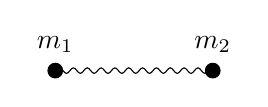
\begin{tikzpicture}
    \fill circle [radius=0.1];
    \fill (2, 0) circle [radius=0.1];
    \node [above] at (0, 0.1) {$m_1$};
    \node [above] at (2, 0.1) {$m_2$};
    \draw [decorate, decoration={snake, amplitude=1, segment length=5}] (0, 0) -- (2, 0);
  \end{tikzpicture}
\end{center}
As we know from classical dynamics, we can decompose the motion into different components:
\begin{itemize}
  \item Translation of the center of mass. We can view this as a single mass with energy $M = m_1 + m_2$.
  \item Rotations about center of mass. There are two axes of rotations orthogonal to the spring, and these have a moment of inertia $I$. We will ignore the rotation along the axes parallel to the spring because we assume the masses are point masses.
  \item Vibrations along the axis of symmetry. The important quantity here is the reduced mass
    \[
      m = \frac{m_1 m_1}{m_1 + m_2}.
    \]
\end{itemize}
We will assume all these motions are independent. In reality, the translation is indeed independent from the others, but the rotations and vibrations can couple in complicated ways. But we are lazy, and will make this simplifying assumption, we have
\[
  Z_1 = Z_{\mathrm{trans}} Z_{\mathrm{rot}} Z_{\mathrm{vib}}.
\]
We can obtain $Z_{\mathrm{trans}}$ just as the partition energy we obtained previously for a single mass, with mass $M$. The remaining two terms depend only on the relative position of the masses. So they do not depend on the molecule as a whole, and are going to be independent of $V$.

Now when we differentiate $\log Z_1$ with respect to $V$, then the latter two terms drop out, and thus we deduce that the ideal gas law still holds for diatomic gases.

We now try to figure out how rotations and vibrations contribute to the partition function. For rotations, we can parametrize this using spherical polars $(\theta, \varphi)$. The Lagrangian for this rotational motion is given by
\[
  \mathcal{L}_{\mathrm{rot}} = \frac{1}{2} I (\dot{\theta}^2 + \sin^2 \theta \dot{\varphi}^2).
\]
The conjugate momenta are given by
\begin{align*}
  p_\theta &= \frac{\partial \mathcal{L}}{\partial \dot{\theta}} = I \dot{\theta}\\
  p_\varphi &= \frac{\partial \mathcal{L}}{\partial \dot{\varphi}} = I \sin^2 \theta \dot\varphi.
\end{align*}
So we have
\[
  H_{\mathrm{rot}} = \dot{\theta} p_\theta + \dot{\varphi} p_\varphi - \mathcal{L}_{\mathrm{rot}} = \frac{p_\theta^2}{2I} + \frac{p_\varphi^2}{2I \sin^2 \theta}.
\]
We can then work out the partition function
\[
  Z_{\mathrm{rot}} = \frac{1}{(2\pi \hbar)^2} \int \d \theta\; \d \varphi\; \d p_\theta \; d p_\varphi\; e^{-\beta H_{\mathrm{rot}}}
\]
We note that the $p_\theta$ and $p_\varphi$ integrals are just Gaussians, and so we get
\[
  Z_{\mathrm{rot}} = \frac{1}{(2\pi \hbar)^2} \sqrt{\frac{2\pi I}{\beta}} \int_0^\pi \d \theta \sqrt{\frac{2\pi I \sin^2 \theta}{\beta}} \int_0^{2\pi} \d \varphi = \frac{2IkT}{\hbar^2}.
\]
Then we get
\[
  E_{\mathrm{rot}} = - \frac{\partial}{\partial \beta} \log Z_{\mathrm{rot}} = \frac{1}{\beta} = kT.
\]
This agrees with the equipartition of energy, as here we have two degrees of freedom, and each contributes $\frac{1}{2}kT$.

\begin{eg}
  In the case of a system where vibrations are not important, e.g.\ if the string is very rigid, then we are done, and we have found
  \[
    Z = Z_{\mathrm{trans}} Z_{\mathrm{rot}} \propto (kT)^{5/2}.
  \]
  Then the partition function for $N$ particles is
  \[
    Z = \frac{1}{N!} Z_1^N.
  \]
  and the total energy is
  \[
    -\frac{\partial}{\partial \beta} \log Z = \frac{5}{2} NkT.
  \]
  This is exactly as we expect. There is $\frac{3}{2}NkT$ from translation, and $NkT$ from rotation. From this, we obtain the heat capacity
  \[
    C_V = \frac{5}{2} Nk.
  \]
\end{eg}
We now put in the vibrations. Since we are modelling it by a spring, we can treat it as a harmonic oscillator, with mass $m$ and frequency $\omega$, which is determined by the bond strength. Then if we let $\zeta$ be the displacement form equilibrium, then the Hamiltonian is
\[
  H_{\mathrm{vib}} = \frac{p_\zeta^2}{2m} + \frac{1}{2}m \omega^2 \zeta^2.
\]
So we have
\[
  Z_{\mathrm{vib}} = \frac{1}{2\pi \hbar} \int \d \zeta\;\d p_\zeta\;e^{-\beta H_{\mathrm{vib}}} = \frac{kT}{\hbar \omega}.
\]
From the partition function, we can get the energy of a single molecule, and find it to be
\[
  E_{\mathrm{vib}} = kT.
\]
This is the average energy in the vibrational motion of a molecule. This looks a bit funny. The vibration is only one degree of freedom, but the equipartition of energy seems to think this has two degrees of freedom. It turns out equipartition of energy behaves differently when we have potential energy. In general, we should think of having one degree of freedom for each quadratic term in the Hamiltonian, and so we have one degree of freedom for kinetic energy and another for potential.

Putting all three types of motion together, we get
\[
  E = \frac{7}{2} NkT,
\]
and the heat capacity is
\[
  C_V = \frac{7}{2}Nk.
\]
Note that these results are completely independent of the parameters describing the molecule!

Does this agree with experiments? The answer is no! If we go and measure the heat capacity of, say, molecular hydrogen, we find something like
\begin{center}
  \begin{tikzpicture}[yscale=0.7]
    \draw [->] (0, 0) -- (5, 0) node [right] {$T$};
    \draw [->] (0, 0) -- (0, 5) node [above] {$C_V/Nk$};

    \draw [dashed] (1.75, 0) node [below] {$200$} -- +(0, 5);
    \draw [dashed] (3.5, 0) node [below] {$2000$} -- +(0, 5);

    \draw [dashed] (0, 1.5) node [left] {$1.5$} -- +(5, 0);
    \draw [dashed] (0, 2.5) node [left] {$2.5$} -- +(5, 0);
    \draw [dashed] (0, 3.5) node [left] {$3.5$} -- +(5, 0);

    \draw [thick, mblue] (0, 1.5) -- (1.5, 1.5) .. controls (1.75, 1.5) and (1.75, 2.5) .. (2, 2.5) -- (3.25, 2.5) .. controls (3.5, 2.5) and (3.5, 3.5) .. (3.75, 3.5) -- (5, 3.5);;
  \end{tikzpicture}
\end{center}
So it seems like our prediction only works when we have high enough temperature. At lower temperatures, the vibration modes freeze out. Then as we further lower the energy, rotation modes also go away. This is a big puzzle classically! This is explained by quantum effects, which we will discuss later.

\subsection{Interacting gases}
So far, we have been talking about ideal gases. What happens if there \emph{are} interactions?

For a real gas, if they are sufficiently dilute, i.e.\ $N/V$ is small, then we expect the interactions to be negligible. This suggests that we can try to capture the effects of interactions perturbatively in $\frac{N}{V}$. We can write the ideal gas law as
\[
  \frac{p}{kT} = \frac{N}{V}.
\]
We can think of this as a first term in an expansion, and add higher order terms
\[
  \frac{p}{kT} = \frac{N}{V} + B_2(T) \frac{N^2}{V^2} + B_3 (T) \frac{N^3}{V^3} + \cdots.
\]
Note that the coefficients depend on $T$ only, as they should be intensive quantities. This is called the \term{Virial expansion}, and the coefficients $B_k(T)$ are the \term{Virial coefficients}. Our goal is to figure out what these $B_k(T)$ are.

We suppose the interaction is given by a potential energy $U(r)$ between two neutral atoms (assuming monoatomic) at separation $r$.

\begin{eg}
  In genuine atoms, for large $r$ (relative to atomic size), we have
  \[
    U(r) \propto -\frac{1}{r^6}.
  \]
  This comes from dipole-dipole interactions. Heuristically, we can understand this power of $6$ as follows --- while the expectation values of electric dipole of an atom vanishes, there exists non-trivial probability that the dipole $p_1$ is non-zero. This gives an electric field of
  \[
    E \sim \frac{p_1}{r^3}.
  \]
  This induces a dipole $p_2$ in atom $2$. So we have
  \[
    p_2 \propto E \sim \frac{p_1}{r^3}.
  \]
  So the resulting potential energy is
  \[
    U \propto -p_2 E \sim -\frac{p_1^2}{r^6}.
  \]
  This is called the \term{van der Waals interaction}. Note that the negative sign means this is an attractive force.

  For small $r$, the electron orbitals of the atoms start to overlap, and then we get repulsion due to the Pauli principle. All together, we obtain the \term{Lennard-Jones potential} given by
  \[
    U(r) = U_0\left(\left(\frac{r_0}{r}\right)^{12} - \left(\frac{r_0}{r}\right)^6\right).
  \]
  \begin{center}
    \begin{tikzpicture}
      \draw [->] (0, 0) -- (5, 0) node [right] {$r$};
      \draw [->] (0, -2) -- (0, 2) node [above] {$U(r)$};

      \draw [mblue, thick ] plot coordinates {(0.955,2.00000) (0.960,1.77280) (0.965,1.47565) (0.970,1.20365) (0.975,0.95482) (0.980,0.72738) (0.985,0.51965) (0.990,0.33010) (0.995,0.15732) (1.000,0.00000) (1.005,-0.14306) (1.010,-0.27298) (1.015,-0.39077) (1.020,-0.49739) (1.025,-0.59370) (1.030,-0.68052) (1.035,-0.75859) (1.040,-0.82859) (1.045,-0.89116) (1.050,-0.94689) (1.055,-0.99632) (1.060,-1.03996) (1.065,-1.07826) (1.070,-1.11165) (1.075,-1.14054) (1.080,-1.16528) (1.085,-1.18622) (1.090,-1.20366) (1.095,-1.21791) (1.100,-1.22922) (1.105,-1.23784) (1.110,-1.24400) (1.115,-1.24792) (1.120,-1.24978) (1.125,-1.24977) (1.130,-1.24806) (1.135,-1.24480) (1.140,-1.24014) (1.145,-1.23420) (1.150,-1.22710) (1.155,-1.21897) (1.160,-1.20990) (1.165,-1.19999) (1.170,-1.18932) (1.175,-1.17799) (1.180,-1.16606) (1.185,-1.15361) (1.190,-1.14069) (1.195,-1.12737) (1.200,-1.11371) (1.205,-1.09974) (1.210,-1.08553) (1.215,-1.07110) (1.220,-1.05650) (1.225,-1.04177) (1.230,-1.02693) (1.235,-1.01202) (1.240,-0.99707) (1.245,-0.98210) (1.250,-0.96712) (1.255,-0.95217) (1.260,-0.93727) (1.265,-0.92242) (1.270,-0.90764) (1.275,-0.89296) (1.280,-0.87837) (1.285,-0.86390) (1.290,-0.84956) (1.295,-0.83534) (1.300,-0.82127) (1.305,-0.80735) (1.310,-0.79358) (1.315,-0.77997) (1.320,-0.76652) (1.325,-0.75325) (1.330,-0.74015) (1.335,-0.72722) (1.340,-0.71448) (1.345,-0.70191) (1.350,-0.68953) (1.355,-0.67733) (1.360,-0.66532) (1.365,-0.65349) (1.370,-0.64184) (1.375,-0.63039) (1.380,-0.61911) (1.385,-0.60803) (1.390,-0.59712) (1.395,-0.58640) (1.400,-0.57586) (1.405,-0.56550) (1.410,-0.55532) (1.415,-0.54531) (1.420,-0.53548) (1.425,-0.52583) (1.430,-0.51635) (1.435,-0.50703) (1.440,-0.49789) (1.445,-0.48891) (1.450,-0.48009) (1.455,-0.47144) (1.460,-0.46294) (1.465,-0.45460) (1.470,-0.44642) (1.475,-0.43838) (1.480,-0.43050) (1.485,-0.42277) (1.490,-0.41518) (1.495,-0.40773) (1.500,-0.40042) (1.530,-0.35940) (1.560,-0.32284) (1.590,-0.29030) (1.620,-0.26131) (1.650,-0.23550) (1.680,-0.21250) (1.710,-0.19198) (1.740,-0.17367) (1.770,-0.15732) (1.800,-0.14268) (1.830,-0.12958) (1.860,-0.11784) (1.890,-0.10729) (1.920,-0.09782) (1.950,-0.08929) (1.980,-0.08160) (2.010,-0.07467) (2.040,-0.06841) (2.070,-0.06275) (2.100,-0.05762) (2.130,-0.05297) (2.160,-0.04875) (2.190,-0.04491) (2.220,-0.04142) (2.250,-0.03824) (2.280,-0.03534) (2.310,-0.03269) (2.340,-0.03027) (2.370,-0.02806) (2.400,-0.02603) (2.430,-0.02417) (2.460,-0.02246) (2.490,-0.02089) (2.520,-0.01945) (2.550,-0.01812) (2.580,-0.01690) (2.610,-0.01577) (2.640,-0.01473) (2.670,-0.01376) (2.700,-0.01287) (2.730,-0.01205) (2.760,-0.01129) (2.790,-0.01058) (2.820,-0.00992) (2.850,-0.00931) (2.880,-0.00875) (2.910,-0.00822) (2.940,-0.00773) (2.970,-0.00727) (3.000,-0.00685) (3.100,-0.00563) (3.200,-0.00465) (3.300,-0.00387) (3.400,-0.00323) (3.500,-0.00272) (3.600,-0.00230) (3.700,-0.00195) (3.800,-0.00166) (3.900,-0.00142) (4.000,-0.00122) (4.100,-0.00105) (4.200,-0.00091) (4.300,-0.00079) (4.400,-0.00069) (4.500,-0.00060) (4.600,-0.00053) (4.700,-0.00046) (4.800,-0.00041) (4.900,-0.00036) (5.000,-0.00032)};

    % map (\x -> (showFFloat (Just 3) x "", showFFloat (Just 5) (min 2 (5 * (1/(x^12) - 1/(x^6)))) "")) [0.955,0.96..1.5]
    % map (\x -> (showFFloat (Just 3) x "", showFFloat (Just 5) (5 * (1/(x^12) - 1/(x^6))) "")) [1.53,1.56..3]
    % map (\x -> (showFFloat (Just 3) x "", showFFloat (Just 5) (5 * (1/(x^12) - 1/(x^6))) "")) [3.1,3.2..5]
    \end{tikzpicture}
  \end{center}
  To make life easy, we will actually use a ``hard core repulsion'' potential instead, given by
  \[
    U(r) =
    \begin{cases}
      \infty & r < r_0\\
      -U_0 \left(\frac{r_0}{r}\right)^6 & r > r_0
    \end{cases}
  \]
  \begin{center}
    \begin{tikzpicture}
      \draw [->] (0, 0) -- (5, 0) node [right] {$r$};
      \draw [->] (0, -2) -- (0, 2) node [above] {$U(r)$};

      \draw [mblue, thick, domain=0.9:5, samples=50] plot [smooth] (\x, {-1/\x^6});

      \draw [mblue, thick] (0.9, -1.8817) -- (0.9, 2);

      \node [anchor = north east] at (0.9, 0) {$r_0$};
    \end{tikzpicture}
  \end{center}
\end{eg}
For a general $U$, we can write the Hamiltonian of the gas is
\[
  H = \sum_{i = 1}^N \frac{\mathbf{p}_i^2}{2m} + \sum_{i > j} U(r_{ij}),
\]
with
\[
  r_{ij} = |\mathbf{r}_i - \mathbf{r}_j|.
\]
is the separation between particle $i$ and particle $j$.

Because of this interaction, it is no longer the case that the partition function for $N$ particles is the $N$th power of the partition function for one particle. We have
\begin{align*}
  Z(N, V, T) &= \frac{1}{N} \frac{1}{(2\pi \hbar)^{3n}} \int \prod_{i = 1}^N \d^3 p_i\; \d^3 r_i e^{-\beta H}\\
  &= \frac{1}{N!} \frac{1}{(2\pi \hbar)^{3n}} \left(\int \prod_{i} \d^3 p_i e^{-\beta p_i^2/2m}\right)\left(\int \prod_i \d^3 r_i\; e^{-\beta \sum_{j < k} U(r_{jk})} \right)\\
  &= \frac{1}{N! \lambda^{3N}} \int \prod_i \d^3 r_i\; e^{-\beta \sum_{j < k} U(r_{jk})},
\end{align*}
where again
\[
  \lambda = \sqrt{\frac{2\pi \hbar^2}{mkT}}.
\]
Since we want to get an expansion, we might want to expand this in terms of the potential, but that is not helpful, because the potential is infinite for small $r$. Instead it is useful to consider the \term{Mayer $f$-function}:
\[
  f(r) = e^{-\beta U(r)} - 1.
\]
This function has the property that $f(r) = -1$ for $r < r_0$ (in the case of the hardcore repulsion), and $f(r) \to 0$ as $r \to \infty$. So this is a nicer function as it only varies within this finite range.

We further simplify notation by defining
\[
  f_{ij} = f(r_{ij}).
\]
Then we have
\begin{align*}
  Z(N, V, T) &= \frac{1}{N! \lambda^{3N}} \left(\int \prod_i \d^3 r_i\prod_{j < k} (1 + f_{jk})\right)\\
  &= \frac{1}{N!\lambda^{3N}} \int \prod_i \d^3 r_i \left(1 + \sum_{j < k} f_{jk} + \sum_{j < k} \sum_{\ell < m} f_{jk} f_{\ell m} + \cdots\right).
\end{align*}
The first term is just
\[
  \int \prod_i \d^3 r_i = V^N,
\]
and this gives the ideal gas term. Now each of the second terms is the same, e.g.\ for $j = 1, k = 2$, this is
\[
  \int \prod_i \d^3 r_i f_{12} = V^{N - 2} \int \d^3 r_1 \; \d^3 r_2\; f_{12} = V^{N - 1} I,
\]
where we set
\[
  I = \int\d^3 r\; f(r).
\]
Since $f(r) \to 0$ as $r \to \infty$, we might as well integrate over all space. Summing over all terms, and approximating $N(N - 1)/2 \sim N^2/2$, we find that the first two terms of the partition function are
\[
  Z(N, V, T) = \frac{V^N}{N! \lambda^{3N}} \left(1 + \frac{N^2}{2V}I + \cdots\right).
\]
Up to first order, we can write this as
\begin{align*}
  Z(N, V, T) &= \frac{V^N}{N! \lambda^{3N}} \left(1 + \frac{N}{2V}I + \cdots\right)^N\\
  &= Z_{\mathrm{ideal}} \left(1 + \frac{N}{2V}I + \cdots \right)^N.
\end{align*}
This pulling out of the $N$ to the exponent might seem a bit arbitrary, but writing it this way, it makes it much clearer that $S$, $F$ etc would be extensive quantities. For example, we can write down the free energy as
\[
  F = -kT \log Z = F_{\mathrm{ideal}} - NkT \log \left(1 + \frac{N}{2V} I + \cdots\right).
\]
Without actually computing $I$, we can expect that it grows as $I \sim r_0^3$. Since we are expanding in terms of $NI/V$, we need
\[
  \frac{N}{V} \ll \frac{1}{r_0^3}.
\]
So we know the expansion is valid if the density of the gas is much less than the density of an atom. In real life, to determine the density of an atom, we need to find a system where the atoms are closely packed. Thus, it suffices to measure the density of the substance in liquid or solid form.

Assuming that the gas is indeed not dense, we can further use the approximation
\[
  \log(1 + x) \approx x.
\]
So we have
\[
  p = - \left(\frac{\partial F}{\partial V}\right)_T = \frac{NkT}{V}\left(1 - \frac{N}{2V} I + \cdots\right).
\]
So we have
\[
  \frac{pV}{NkT} = 1 - \frac{N}{2V} I + \cdots.
\]
So we can now read off what the second Virial coefficient is:
\[
  B_2 = -\frac{1}{2} I.
\]
We can consider what we get with different potentials. If we have a completely repulsive potential, then $U(r) > 0$ everywhere. So $f < 0$, and thus $B_2(t) > 0$. In other words, having a repulsive interaction tends to increase the pressure, which makes sense. On the other hand, if we have an attractive potential, then the pressure decreases.

If we have a hardcore repulsion, then we have
\[
  I = \int_{r = 0}^{r = r_0} \d^3 r\; (-1) + \int_{r = r_0}^\infty \d^3 r\; \left(e^{\beta U_0 (r_0/r)^6} - 1\right).
\]
The second term is slightly tricky, so we'll restrict to the case of high temperature, hence small $\beta$. We can write
\[
  e^{\beta U_0 (r_0/r)^6} \approx 1 + \beta U_0 \left(\frac{r_0}{r}\right)^6 + \cdots
\]
Then we get
\[
  I \approx \frac{4}{3}\pi r_0^3 +\frac{4 \pi U_0}{kT} \int_{r_0}^\infty \d r\; \frac{r_0^6}{r^6} = \frac{4\pi r_0^3}{3}\left(\frac{U_0}{kT} - 1\right).
\]
For large $T$, this is negative, and so the repulsive interaction dominates. We can plug this into our equation of state, and find
\[
  \frac{pV}{NkT} \approx 1 - \frac{N}{V}\left(\frac{a}{kT} - b\right),
\]
where
\[
  a = \frac{2\pi r_0^3}{3}U_0,\quad b = \frac{2\pi r_0^3}{3}.
\]
We can invert this to get
\[
  kT = \frac{V}{N}\left(p + \frac{N^2}{V^2} a\right) \left(1 + \frac{N}{V}b\right)^{-1}.
\]
Taking the Taylor expansion of the inverse and truncating higher order terms, we obtain
\[
  kT = \left(p + \frac{N^2}{V^2}a \right)\left(\frac{V}{N} - b\right).
\]
This is the \term{van der Waals equation of state}\index{equation of state!van der waals}, which is valid at low density ($Nr_0^3/V \ll 1$) and high temperature ($\beta U_0 \ll 1$).

We can also write this as
\[
  p = \frac{NkT}{V - bN} - a \frac{N^2}{V^2}.
\]
In this form, we see that $a$ gives a reduced pressure due to long distance attractive force, while we can view the $b$ contribution as saying that the atoms take up space, and hence reduces the volume.

By why exactly the factor of $bN$? Imagine two atoms living right next to each other.
\begin{center}
  \begin{tikzpicture}[scale=0.5]
    \draw circle [radius=1];
    \draw (2, 0) circle [radius=1];
    \draw [dashed] circle [radius=2];

    \draw (0, 0) node [circ] {} -- (2, 0) node [circ] {} node [pos=0.3, above] {$r_0$};
  \end{tikzpicture}
\end{center}
The value $r_0$ was chosen to be the distance between the two cores, so the volume of each atom is
\[
  \frac{4\pi}{3}\left(\frac{r_0}{2}\right)^3,
\]
which is not $b$. We might think the right way to do this problem is to look at how much volume the atom excludes, i.e.\ the dashed volume. This is
\[
  \Omega = \frac{4}{3}\pi r_0^3 = 2b.
\]
This is again not right. So we probably want to think more carefully.

Suppose we have $N$ particles. When we put in the first atom, the amount of space available to put it is $V$. When we now try to put in the second, the available space is $V - \Omega$ (assuming the two atoms are not too close together so that they don't exclude the same volume). Similarly, when we put in the third, the available space is $V - 2 \Omega$.

Diving by $N!$ for indistinguishability, we find that the total phase space volume available for placing our particles is
\begin{align*}
  \frac{1}{N!}V(V - \Omega) (V -2\Omega) \cdots (V - (N - 1) \Omega) &\approx \frac{1}{N!} V^N\left(1 - \frac{N^2}{2} \frac{\Omega}{V} + \cdots\right)\\
  &\approx \frac{1}{N!} \left(V - \frac{N\Omega}{2}\right)^N,
\end{align*}
which explains why the reduced volume for each particle is $\Omega/2$ instead of $\Omega$.

Now suppose we want to find higher-order corrections to the partition function in the Virial expansion. The obvious thing might be to take them to be the contributions by $\sum \sum f_{jk} f_{\ell m}$. However, this is not quite right. If we try to keep track of how large the terms are carefully, we will get a different answer.

The way to do it properly would be via the \term{cluster expansion}, which involves using nice diagrams to figure out the right terms to include, similar to how Feynman diagrams are used to do perturbation theory in quantum field theory. Unfortunately, we do not have the time to go into the details.

\section{Quantum gases}
We now move on to study quantum gases. As before, we are going to spend a lot of time evaluating the partition function for different systems. Recall that the partition function is defined as a sum over all eigenstates. In the world of classical gases, we had the benefit of working over a continuous phase space, and thus we can replace the sum by integrals. In the quantum world, this is no longer the case, However, most of the time, the states are very closely packed, and we might as well approximate the sum by an integral. Of course, we cannot replace the sum just by $\int \d E$. We have to make sure we preserve the ``density'' of the energy levels.

\subsection{Density of states}
Consider an ideal gas in a cubic box with side lengths $L$. So we have $V = L^3$. Since there are no interactions, the wavefunction for multiple states can be obtained from the wavefunction of single particle states,
\[
  \psi(\mathbf{x}) = \frac{1}{\sqrt{V}} e^{i\mathbf{k}\cdot \mathbf{x}}.
\]
We impose periodic boundary conditions, so the wavevectors are quantized by
\[
  k_i = \frac{2\pi n_i}{L},
\]
with $n_i \in \Z$.

The one-particle energy is given by
\[
  E_\mathbf{n} = \frac{\hbar^2 \mathbf{k}^2}{2m} = \frac{4\pi^2 \hbar^2}{2mL^2}(n_1^2 + n_2^2 + n_3^2).
\]
So if we are interested in a one-particle partition function, we have
\[
  Z_1 = \sum_\mathbf{n} e^{-\beta E_\mathbf{n}}.
\]
We now note that
\[
  \beta E_n \sim \frac{\lambda^2}{L^2}\mathbf{n}^2,
\]
where
\[
  \lambda = \sqrt{\frac{2\pi \hbar^2}{mkT}}.
\]
is the de Broglie wavelength.

This $\frac{\lambda^2}{L^2}$ gives the spacing between the energy levels. But we know that $\lambda \ll L$. So the energy levels are very finely spaced, and we can replace the sum by an integral. Thus we can write
\[
  \sum_\mathbf{n} \approx \int \d^3 \mathbf{n} \approx \frac{V}{(2\pi)^3} \int \d^3 \mathbf{k} \approx \frac{4\pi V}{(2\pi)^3} \int_0^\infty \d |\mathbf{k}|\; |\mathbf{k}|^2,
\]
where in the last step, we replace with spherical polars and integrated over angles. The final step is to replace $|\mathbf{k}|$ by $E$. We know that
\[
  E = \frac{\hbar^2 |\mathbf{k}|^2}{2m}.
\]
So we get that
\[
  \d E = \frac{\hbar^2 |\mathbf{k}|}{m} \d |\mathbf{k}|.
\]
Therefore we can write
\[
  \sum_\mathbf{n} = \frac{4\pi V}{(2\pi)^3} \int_0^\infty \d E\; \sqrt{\frac{2mE}{\hbar^2}}\frac{m}{\hbar^2}.
\]
We then set
\[
  g(E) = \frac{V}{2\pi^2} \left(\frac{2m}{\hbar^2}\right)^{3/2} E^{1/2}.
\]
This is called the \term{density of states}. Approximately, $g(E) \;\d E$ is the number of single particle states with energy between $E$ and $E + \d E$. Then we have
\[
  \sum_\mathbf{n} = \int g(E)\;\d E.
\]
The same result (and derivation) holds if the sides of the box have different length. In general, in $d$ dimensions, the density of states is given by
\[
  g(E) = \frac{V \vol(S^{d - 1})}{2\cdot \pi^{d/2}} \left(\frac{m}{2\pi \hbar^2}\right)^{d/2} E^{d/2 - 1}.
\]
All these derivations work if we have a non-relativistic free particle, since we assumed the \term{dispersion relation} between $E$ and $\mathbf{k}$, namely
\[
  E = \frac{\hbar^2 |\mathbf{k}|^2}{2m}.
\]
For a relativistic particle, we instead have
\[
  E = \sqrt{\hbar^2 |\mathbf{k}|^2 c^2 + m^2c^4}.
\]
In this case, $|\mathbf{k}|$ is still quantized as before, and repeating the previous argument, we find that
\[
  g(E) = \frac{VE}{2\pi^3 \hbar^3 c^3} \sqrt{E^2 - m^2 c^4}.
\]
We will be interested in the special case where $m = 0$. Then we simply have
\[
  g(E) = \frac{VE^2}{2\pi^3 \hbar^3 c^3}.
\]
We can start doing some physics with this.

\subsection{Black-body radiation}
Unfortunately, in this chapter, we do not have much opportunity to deal with genuine gases. Instead, we are going to take some system that is \emph{not} a gas, and pretend it is a gas. Of course, nothing in our previous derivations relied on the system actually being a gas. It just relied on the fact that we had a lot of things. So the results should still hold.

In this chapter, we suppose have a gas of photons (which is just a fancy way to say ``photons'') in a box with opaque walls.
\begin{center}
  \begin{tikzpicture}[photon/.style={morange!50!black, decorate, decoration={snake, amplitude=1, segment length=3, post=lineto, post length=3}, -latex'}]
    \draw [thick] (0, 0) rectangle (2, 2);

    \draw [photon] (0.3, 1.7) -- +(0.4, -0.2);
    \draw [photon] (1, 0.7) -- +(0.05, 0.5);

    \draw [photon] (0.2, 0.3) -- +(0.5, -0.05);
    \draw [photon] (1.7, 0.7) -- +(0, 0.55);
    \draw [photon] (1.8, 0.2) -- +(-0.3, 0.3);
    \draw [photon] (0.2, 1) -- +(0.55, 0);
    \draw [photon] (1.7, 1.8) -- +(-0.4, -0.2);
  \end{tikzpicture}
\end{center}
We suppose this box of photon is at equilibrium with temperature $T$. We will use the box of photons as a model of a ``\term{black body}'', i.e.\ a perfectly absorbing object. The gas of photons inside is called \term{black-body radiation}.
 Later on, we will argue that the photons emitted by a black body must indeed follow the same distribution as the photons inside our box.

We begin by reminding ourselves of some basic properties of photons: they are massless and have energy
\[
  E = \hbar \omega,\quad \omega = \frac{2\pi c}{\lambda},
\]
and $\lambda$ is the (genuine) wavelength of the photon.

Interactions between photons are negligible, so we can treat them as noble gas.

Photons have two polarization states, since given any direction of travel $\mathbf{k}$, the electric and magnetic fields have to obey
\[
  \mathbf{E} \cdot \mathbf{k} = \mathbf{B} \cdot \mathbf{k} = \mathbf{B} \cdot \mathbf{E} = 0,
\]
and there are two independent choices for $\mathbf{E}$ and $\mathbf{B}$. This has implications for our counting, as we need an extra factor of $2$ in our density of states. So the density of states is given by
\[
  g(E) \;\d E = \frac{VE^2}{\pi^2 \hbar^3 c^3}\;\d E.
\]
Using the fact that
\[
  E = \hbar \omega,
\]
it is often convenient to instead write this as
\[
  g(\omega)\; \d \omega = \frac{V \omega^2}{\pi^2 c^3}\;\d \omega.
\]
This is an abuse of notation, as the two $g$'s we wrote down are different functions, but this is a physics course.

The final important property of the photons is that photon numbers are not conserved. Indeed, they are absorbed and emitted by walls of the box. So we must sum over all possible photon numbers, even though we are in the canonical ensemble. In practice, what we get is the same as the grand canonical ensemble, but with $\mu = 0$.

We can begin. While we have figured out the density of states, we will not use that immediately. Instead, we still begin by assuming that we have a discrete set of states. Only after doing all the manipulations, we replace all remaining occurrences of sums with integrals so that we can actually evaluate it.

We can work with this in more generality. Consider a system of non-interacting particles with one-particle states $\bket{i}$ of energies $E_i$. Then the general accessible state can be labelled by
\[
  \{n_1, n_2, \cdots\},
\]
where $n_i$ is the number of particles in $\bket{i}$. Since particle numbers are not conserved, we do not impose any restrictions on the possible values of the $n_i$. The energy of such a state is just
\[
  \sum_i n_i E_i.
\]
As before, in the canonical ensemble, the probability of being in such a state is
\[
  p(\{n_i\}) = \frac{1}{Z} e^{-\beta \sum n_j E_j},
\]
and
\[
  Z = \sum_{\{n_k\}} e^{-\beta \sum n_j E_j} = \sum_{n_1 = 0}^\infty e^{-\beta n_1 E_1} \sum_{n = 2}^\infty e^{-\beta n_2 E_2} \cdots = \prod_i \frac{1}{1 - e^{-\beta E_i}}.
\]
So we find that
\[
  \log Z = - \sum_i \log (1 - e^{-\beta E_i}).
\]
Using this, we have
\begin{align*}
  \bra n_i\ket &= \sum_{\{n_k\}} n_i p (\{n_k\}) \\
  &= \sum_{\{n_k\}} \frac{n_i e^{-\beta \sum_j n_j E_j}}{Z}\\
  &= - \frac{1}{\beta} \frac{\partial}{\partial E_i} \log Z.
\end{align*}
Using the formula of $\log Z$ we had, we find
\[
  \bra n_i\ket = \frac{1}{e^{\beta E_i} - 1}.
\]
Applying this to photons, we replace the sum with an integral, and $E_i = \hbar \omega$. Using our density of states, we have
\[
  \log Z = - \frac{V}{\pi^3 c^3} \int_0^\infty \d \omega\; \omega^2 \log(1 - e^{-\beta \hbar \omega}).
\]
Similarly, the average number of photons with frequency between $\omega$ and $\d \omega$ is
\[
  n(\omega)\; \d \omega = g(\omega) \;\d \omega \cdot \frac{1}{e^{\beta \hbar \omega} - 1} = \frac{V \omega^2\;\d \omega}{\pi^2 c^3(e^{\beta\hbar\omega} - 1)}.
\]
Thus, the total energy in this range is
\[
  E(\omega) \;\d \omega = \hbar \omega n(\omega) \;\d \omega = \frac{V \hbar}{\pi^2 c^3} \frac{\omega^3}{e^{\beta \hbar \omega} - 1}\;\d \omega.
\]
This is the \term{Planck distribution}.

Let's check that this makes sense. Let's try to compute the total energy of all photons. We have
\[
  E = -\left(\frac{\partial \log Z}{\partial \beta}\right)_V = \frac{V \hbar}{\pi^2 c^3}\int_0^\infty \d \omega\; \frac{\omega^3}{e^{\beta \hbar \omega} - 1} = \int_0^\infty E(\omega) \;\d \omega,
\]
as we would expect.

Putting $\omega = \frac{2\pi c}{\lambda}$, we find that the average energy with wavelength between $\lambda$ and $\lambda + \d \lambda$ is given by the horrendous formula
\[
  \tilde{E} (\lambda) \;\d \lambda = \frac{V \hbar (2\pi c)^4}{\pi^2 c^3 \lambda^5} \frac{\d \lambda}{e^{\beta \hbar 2 \pi c/\lambda} - 1}.
\]
We can plot this for some values of $T$:
\begin{center}
  \begin{tikzpicture}[xscale=3]
    \draw [->] (0, 0) -- (2, 0) node [right] {$\lambda$};

    \draw [->] (0, 0) -- (0, 4) node [above] {$E(\lambda)$};

    \draw [mred, thick] plot coordinates {(0.01,0.00000) (0.03,0.00000) (0.05,0.00000) (0.07,0.00000) (0.09,0.00000) (0.11,0.00000) (0.13,0.00010) (0.15,0.00109) (0.17,0.00611) (0.19,0.02244) (0.21,0.06120) (0.23,0.13450) (0.25,0.25167) (0.27,0.41663) (0.29,0.62717) (0.31,0.87585) (0.33,1.15188) (0.35,1.44304) (0.37,1.73730) (0.39,2.02399) (0.41,2.29438) (0.43,2.54192) (0.45,2.76219) (0.47,2.95266) (0.49,3.11234) (0.51,3.24152) (0.53,3.34137) (0.55,3.41373) (0.57,3.46083) (0.59,3.48514) (0.61,3.48919) (0.63,3.47550) (0.65,3.44649) (0.67,3.40444) (0.69,3.35144) (0.71,3.28941) (0.73,3.22004) (0.75,3.14488) (0.77,3.06525) (0.79,2.98233) (0.81,2.89713) (0.83,2.81052) (0.85,2.72324) (0.87,2.63592) (0.89,2.54907) (0.91,2.46314) (0.93,2.37848) (0.95,2.29538) (0.97,2.21406) (0.99,2.13472) (1.01,2.05748) (1.03,1.98244) (1.05,1.90968) (1.07,1.83922) (1.09,1.77111) (1.11,1.70532) (1.13,1.64185) (1.15,1.58068) (1.17,1.52177) (1.19,1.46506) (1.21,1.41052) (1.23,1.35808) (1.25,1.30769) (1.27,1.25928) (1.29,1.21279) (1.31,1.16816) (1.33,1.12531) (1.35,1.08419) (1.37,1.04473) (1.39,1.00687) (1.41,0.97054) (1.43,0.93569) (1.45,0.90225) (1.47,0.87016) (1.49,0.83938) (1.51,0.80984) (1.53,0.78149) (1.55,0.75429) (1.57,0.72818) (1.59,0.70312) (1.61,0.67906) (1.63,0.65596) (1.65,0.63378) (1.67,0.61247) (1.69,0.59201) (1.71,0.57235) (1.73,0.55346) (1.75,0.53530) (1.77,0.51785) (1.79,0.50108) (1.81,0.48494) (1.83,0.46943) (1.85,0.45450) (1.87,0.44014) (1.89,0.42633) (1.91,0.41303) (1.93,0.40022) (1.95,0.38789) (1.97,0.37602) (1.99,0.36458)};
    \draw [mred!75!mblue, thick] plot coordinates {(0.01,0.00000) (0.03,0.00000) (0.05,0.00000) (0.07,0.00000) (0.09,0.00000) (0.11,0.00000) (0.13,0.00000) (0.15,0.00002) (0.17,0.00018) (0.19,0.00095) (0.21,0.00351) (0.23,0.00990) (0.25,0.02283) (0.27,0.04515) (0.29,0.07922) (0.31,0.12643) (0.33,0.18696) (0.35,0.25984) (0.37,0.34317) (0.39,0.43442) (0.41,0.53075) (0.43,0.62931) (0.45,0.72742) (0.47,0.82274) (0.49,0.91332) (0.51,0.99764) (0.53,1.07459) (0.55,1.14345) (0.57,1.20381) (0.59,1.25557) (0.61,1.29883) (0.63,1.33386) (0.65,1.36107) (0.67,1.38097) (0.69,1.39409) (0.71,1.40103) (0.73,1.40238) (0.75,1.39871) (0.77,1.39061) (0.79,1.37861) (0.81,1.36323) (0.83,1.34492) (0.85,1.32414) (0.87,1.30127) (0.89,1.27669) (0.91,1.25071) (0.93,1.22363) (0.95,1.19571) (0.97,1.16717) (0.99,1.13822) (1.01,1.10904) (1.03,1.07978) (1.05,1.05056) (1.07,1.02152) (1.09,0.99274) (1.11,0.96431) (1.13,0.93629) (1.15,0.90875) (1.17,0.88173) (1.19,0.85528) (1.21,0.82941) (1.23,0.80415) (1.25,0.77953) (1.27,0.75555) (1.29,0.73221) (1.31,0.70953) (1.33,0.68750) (1.35,0.66611) (1.37,0.64537) (1.39,0.62527) (1.41,0.60578) (1.43,0.58692) (1.45,0.56865) (1.47,0.55097) (1.49,0.53387) (1.51,0.51733) (1.53,0.50133) (1.55,0.48587) (1.57,0.47092) (1.59,0.45648) (1.61,0.44252) (1.63,0.42903) (1.65,0.41599) (1.67,0.40340) (1.69,0.39123) (1.71,0.37948) (1.73,0.36812) (1.75,0.35716) (1.77,0.34656) (1.79,0.33632) (1.81,0.32643) (1.83,0.31687) (1.85,0.30763) (1.87,0.29871) (1.89,0.29008) (1.91,0.28175) (1.93,0.27369) (1.95,0.26590) (1.97,0.25837) (1.99,0.25109)};
    \draw [mred!50!mblue, thick] plot coordinates {(0.01,0.00000) (0.03,0.00000) (0.05,0.00000) (0.07,0.00000) (0.09,0.00000) (0.11,0.00000) (0.13,0.00000) (0.15,0.00000) (0.17,0.00000) (0.19,0.00002) (0.21,0.00013) (0.23,0.00047) (0.25,0.00139) (0.27,0.00338) (0.29,0.00709) (0.31,0.01322) (0.33,0.02241) (0.35,0.03516) (0.37,0.05174) (0.39,0.07217) (0.41,0.09624) (0.43,0.12354) (0.45,0.15350) (0.47,0.18547) (0.49,0.21877) (0.51,0.25270) (0.53,0.28661) (0.55,0.31991) (0.57,0.35209) (0.59,0.38274) (0.61,0.41150) (0.63,0.43812) (0.65,0.46243) (0.67,0.48432) (0.69,0.50373) (0.71,0.52066) (0.73,0.53515) (0.75,0.54728) (0.77,0.55713) (0.79,0.56484) (0.81,0.57053) (0.83,0.57433) (0.85,0.57639) (0.87,0.57685) (0.89,0.57585) (0.91,0.57354) (0.93,0.57003) (0.95,0.56547) (0.97,0.55997) (0.99,0.55365) (1.01,0.54660) (1.03,0.53893) (1.05,0.53072) (1.07,0.52206) (1.09,0.51303) (1.11,0.50369) (1.13,0.49410) (1.15,0.48433) (1.17,0.47441) (1.19,0.46440) (1.21,0.45434) (1.23,0.44426) (1.25,0.43420) (1.27,0.42418) (1.29,0.41423) (1.31,0.40436) (1.33,0.39461) (1.35,0.38497) (1.37,0.37548) (1.39,0.36613) (1.41,0.35694) (1.43,0.34792) (1.45,0.33907) (1.47,0.33040) (1.49,0.32191) (1.51,0.31360) (1.53,0.30549) (1.55,0.29755) (1.57,0.28981) (1.59,0.28226) (1.61,0.27489) (1.63,0.26770) (1.65,0.26071) (1.67,0.25389) (1.69,0.24725) (1.71,0.24078) (1.73,0.23449) (1.75,0.22837) (1.77,0.22242) (1.79,0.21663) (1.81,0.21100) (1.83,0.20553) (1.85,0.20021) (1.87,0.19504) (1.89,0.19001) (1.91,0.18513) (1.93,0.18038) (1.95,0.17577) (1.97,0.17129) (1.99,0.16693)};

    \draw [mred!25!mblue, thick] plot coordinates {(0.01,0.00000) (0.03,0.00000) (0.05,0.00000) (0.07,0.00000) (0.09,0.00000) (0.11,0.00000) (0.13,0.00000) (0.15,0.00000) (0.17,0.00000) (0.19,0.00000) (0.21,0.00000) (0.23,0.00001) (0.25,0.00004) (0.27,0.00012) (0.29,0.00032) (0.31,0.00072) (0.33,0.00147) (0.35,0.00269) (0.37,0.00454) (0.39,0.00718) (0.41,0.01072) (0.43,0.01523) (0.45,0.02077) (0.47,0.02733) (0.49,0.03485) (0.51,0.04326) (0.53,0.05244) (0.55,0.06226) (0.57,0.07257) (0.59,0.08321) (0.61,0.09404) (0.63,0.10491) (0.65,0.11569) (0.67,0.12625) (0.69,0.13649) (0.71,0.14632) (0.73,0.15567) (0.75,0.16446) (0.77,0.17267) (0.79,0.18025) (0.81,0.18719) (0.83,0.19347) (0.85,0.19910) (0.87,0.20407) (0.89,0.20841) (0.91,0.21213) (0.93,0.21526) (0.95,0.21781) (0.97,0.21982) (0.99,0.22132) (1.01,0.22234) (1.03,0.22290) (1.05,0.22305) (1.07,0.22281) (1.09,0.22221) (1.11,0.22128) (1.13,0.22005) (1.15,0.21855) (1.17,0.21680) (1.19,0.21483) (1.21,0.21266) (1.23,0.21032) (1.25,0.20781) (1.27,0.20518) (1.29,0.20242) (1.31,0.19956) (1.33,0.19661) (1.35,0.19359) (1.37,0.19051) (1.39,0.18738) (1.41,0.18421) (1.43,0.18102) (1.45,0.17781) (1.47,0.17459) (1.49,0.17137) (1.51,0.16815) (1.53,0.16494) (1.55,0.16175) (1.57,0.15858) (1.59,0.15544) (1.61,0.15233) (1.63,0.14924) (1.65,0.14620) (1.67,0.14319) (1.69,0.14023) (1.71,0.13730) (1.73,0.13443) (1.75,0.13159) (1.77,0.12881) (1.79,0.12607) (1.81,0.12338) (1.83,0.12074) (1.85,0.11815) (1.87,0.11561) (1.89,0.11311) (1.91,0.11067) (1.93,0.10828) (1.95,0.10594) (1.97,0.10364) (1.99,0.10140)};

    \draw [mblue, thick] plot coordinates {(0.01,0.00000) (0.03,0.00000) (0.05,0.00000) (0.07,0.00000) (0.09,0.00000) (0.11,0.00000) (0.13,0.00000) (0.15,0.00000) (0.17,0.00000) (0.19,0.00000) (0.21,0.00000) (0.23,0.00000) (0.25,0.00000) (0.27,0.00000) (0.29,0.00001) (0.31,0.00003) (0.33,0.00007) (0.35,0.00015) (0.37,0.00030) (0.39,0.00055) (0.41,0.00093) (0.43,0.00149) (0.45,0.00225) (0.47,0.00326) (0.49,0.00453) (0.51,0.00609) (0.53,0.00795) (0.55,0.01011) (0.57,0.01255) (0.59,0.01528) (0.61,0.01825) (0.63,0.02145) (0.65,0.02483) (0.67,0.02837) (0.69,0.03203) (0.71,0.03576) (0.73,0.03954) (0.75,0.04332) (0.77,0.04708) (0.79,0.05078) (0.81,0.05440) (0.83,0.05791) (0.85,0.06130) (0.87,0.06454) (0.89,0.06762) (0.91,0.07053) (0.93,0.07327) (0.95,0.07581) (0.97,0.07817) (0.99,0.08033) (1.01,0.08230) (1.03,0.08409) (1.05,0.08568) (1.07,0.08709) (1.09,0.08833) (1.11,0.08939) (1.13,0.09028) (1.15,0.09102) (1.17,0.09160) (1.19,0.09204) (1.21,0.09235) (1.23,0.09252) (1.25,0.09257) (1.27,0.09251) (1.29,0.09234) (1.31,0.09207) (1.33,0.09171) (1.35,0.09126) (1.37,0.09073) (1.39,0.09014) (1.41,0.08947) (1.43,0.08875) (1.45,0.08797) (1.47,0.08714) (1.49,0.08626) (1.51,0.08535) (1.53,0.08440) (1.55,0.08342) (1.57,0.08241) (1.59,0.08137) (1.61,0.08032) (1.63,0.07925) (1.65,0.07816) (1.67,0.07707) (1.69,0.07596) (1.71,0.07485) (1.73,0.07373) (1.75,0.07261) (1.77,0.07148) (1.79,0.07036) (1.81,0.06925) (1.83,0.06813) (1.85,0.06702) (1.87,0.06592) (1.89,0.06482) (1.91,0.06374) (1.93,0.06266) (1.95,0.06159) (1.97,0.06053) (1.99,0.05949)};
     %% mapM_ (\n -> print $ map (\x -> (showFFloat (Just 2) x "", showFFloat (Just 5) (24 / (x^5 * (exp(n / x) - 1))) "")) ([0.01,0.03..2])) [3, 3.9, 5, 6.6, 8.6]
  \end{tikzpicture}
\end{center}
Note that the maximum shifts to the right as temperature lowers, and the total energy released also decreases. For the maximum to be near the visible range, we need $T \sim \SI{6000}{\kelvin}$, which is quite a lot.

In general, if we want to figure out when $E(\omega)$ is maximized, then we set
\[
  \frac{\d E}{\d \omega} = 0.
\]
This gives us
\[
  \omega_{\mathrm{max}} = \zeta \frac{kT}{\hbar},
\]
where $\zeta \approx 2.822$ is the solution to
\[
  3 - \zeta = 3 e^{-\zeta}.
\]
This is known as \term{Wien's displacement law}. In particular, we see that this is linear in $T$.

Recall that we didn't actually find the value of $E$. To do so, we have to do the integral. We perform the change of variables $x = \beta \hbar \omega$ to get
\[
  E = \frac{V(kT)^4}{\pi^2 c^3 \hbar^3} \int_0^\infty \frac{x^3\;\d x}{e^x - 1}.
\]
The remaining integral is just some constant, which isn't really that important, but it happens that we can actually evaluate it, and find the value to be
\[
  \int_0^\infty \frac{x^3\; \d x}{e^x - 1} = \Gamma(4) \zeta(4) = \frac{\pi^4}{15},
\]
where $\zeta$ is the \term{Riemann zeta function}.

The energy density of the box is thus
\[
  \mathcal{E} = \frac{E}{V} = \frac{\pi^2 k^4}{15 \hbar^3 c^3} T^4 \propto T^4.
\]
Now if we are experimentalists, then we have no way to figure out if the above result is correct, because the box is all closed. To look into the box, we cut a small hole in the box:
\begin{center}
  \begin{tikzpicture}[photon/.style={morange!50!black, decorate, decoration={snake, amplitude=1, segment length=3, post=lineto, post length=3}, -latex'}]
    \draw [thick] (0, 0) rectangle (2, 2);

    \draw [photon] (0.3, 1.7) -- +(0.4, -0.2);
    \draw [photon] (1, 0.7) -- +(0.05, 0.5);

    \draw [photon] (0.2, 0.3) -- +(0.5, -0.05);
    \draw [photon] (1.7, 0.7) -- +(0, 0.55);
    \draw [photon] (1.8, 0.2) -- +(-0.3, 0.3);
    \draw [photon] (0.2, 1) -- +(0.55, 0);
    \draw [photon] (1.7, 1.8) -- +(-0.4, -0.2);

    \fill [white] (1.95, 0.95) rectangle (2.05, 1.05);
  \end{tikzpicture}
\end{center}
Let's say this hole has area $A$, which is sufficiently small that it doesn't mess with what is going on in the box. How much energy do we expect the box to leak out of the hole?

For the purposes of this analysis, for a wave vector $\mathbf{k}$, we let $S(\mathbf{k})$ be the set of all photons with wave-vector within $\d^3 \mathbf{k}$ of $\mathbf{k}$. We further suppose $\mathbf{k}$ makes an angle $\theta$ with the normal to the hole.
\begin{center}
  \begin{tikzpicture}
    \draw [thick] (0, 0) -- (0, 2);

    \fill [white] (-0.05, 0.8) rectangle (0.05, 1.2);

    \draw [mred, -latex'] (-1, 1.7) -- +(0.6, -0.45) node [pos=0.5, anchor=south west] {$\mathbf{k}$};

    \draw [dashed] (-0.4, 1.25) -- +(-0.7, 0);

    \draw (-0.7, 1.25) arc(180:143:0.3);:

    \draw (-0.7, 0.6) node [right] {$\theta$} edge [out=180, in=180, -latex'] (-0.685, 1.345);
  \end{tikzpicture}
\end{center}
What we want to know is what portion of $S(\mathbf{k})$ manages to get out of the hole, say in a time period $\d t$. To do so, we look at the following volume:
\begin{center}
  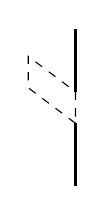
\begin{tikzpicture}
    \draw [thick] (0, 0) -- (0, 2);

    \fill [white] (-0.05, 0.8) rectangle (0.05, 1.2);

    \draw [dashed] (0, 0.8) -- (-0.6, 1.25) -- (-0.6, 1.65) -- (0, 1.2) -- cycle;
  \end{tikzpicture}
\end{center}
The volume of this box is $A c \cos \theta \;\d t$. So the proportion of energy that gets out is simply
\[
  \frac{A c \cos \theta}{V} \;\d t.
\]
We now write
\[
  E(|\mathbf{k}|) \;\d^3 \mathbf{k} = \text{total energy in $S(\mathbf{k})$}.
\]
Then the total energy leaving the hole in time $\d t$ as
\[
  \int_{\theta \in [0, \pi/2]} \d^3 \mathbf{k}\; \frac{A c \cos \theta}{V}\;\d t\; E(|\mathbf{k}|).
\]
To evaluate this integrate, we simply have to introduce polar coordinates, and we get
\[
  \frac{cA \;\d t}{V} \int_0^{2\pi}\d \varphi \int_0^{\pi/2} \d \theta \sin \theta \cos \theta \int_0^\infty \d |\mathbf{k}|\; |\mathbf{k}|^2 E(|\mathbf{k}|).
\]
The first two integrals give $2\pi$ and $\frac{1}{2}$ respectively, and we can rewrite the last integral back into Cartesian coordinates, and it is
\[
  \frac{1}{4\pi}\int \d^3 \mathbf{k}\; E(|\mathbf{k}|) = \frac{E}{4\pi}.
\]
Putting these all together, we find that the rate of energy emission is
\[
  \frac{1}{4} cA \mathcal{E} \;\d t.
\]
If we define the \term{energy flux} as energy per unit time per unit area leaving the hole, then the energy flux is given by
\[
  \frac{c}{4} \mathcal{E} = \sigma T^4,
\]
where
\[
  \sigma = \frac{\pi^2 k^4}{60 \hbar^3 c^2} \approx \SI{5.67e-8}{\joule\per\second\per\meter\squared\per\kelvin\tothe{-4}}.
\]
What was the point of computing this? We don't really care that much about the experimentalists. Suppose we had any black body, and we want to figure out how much radiation it is emitting. We imagine we put it inside that box. Then to the box, the surface of the black body is just like the hole we drilled through the box. So we know that the black body is absorbing $\sigma T^4$ energy per unit time per unit area.

But the system is in equilibrium, so the black body must emit the exact same amount of radiation out. So what we have derived is in fact how black bodies behave!

The best example of a black body we know of is the cosmic background microwave radiation of the universe. This is a black body radiation to incredibly high accuracy, with a temperature of $T = \SI{2.7}{\kelvin}$. This is the temperature of space.

Let's quickly calculate some other thermodynamic quantities we might be interested in. We have
\begin{align*}
  F &= - kT \log Z\\
  &= -\frac{VkT}{\pi^2 c^3}\int_0^\infty \d \omega\; \omega^2 \log (1 - e^{-\beta \hbar \omega})\\
  \intertext{Integrating by parts, we obtain}
  &= -\frac{V \hbar}{3\pi^2 c^3}\int_0^\infty \d \omega\; \frac{\omega^3 e^{-\beta \hbar \omega}}{1 - e^{-\beta \hbar \omega}}\\
  &= - \frac{V \hbar}{3\pi^2 c^3} \frac{1}{\beta^4 \hbar^4} \int_0^\infty \frac{x^3 \;\d x}{e^x - 1} \\
  &= - \frac{V \pi^2 k^4}{45 \hbar^3 c^3}T^4.
\end{align*}
The free energy is useful, because we can differentiate it to get pressure:
\[
  p = - \left(\frac{\partial F}{\partial V}\right)_T = \frac{E}{3V} = \frac{1}{3}\mathcal{E} = \frac{4\sigma}{3c} T^4.
\]
This is \term{radiation pressure}. Since $c$ is a big number, we see that radiation pressure is small.

We can also get the entropy from this. We compute
\[
  S = -\left(\frac{\partial F}{\partial T}\right)_V = \frac{16 V \sigma}{3c}T^3.
\]
Another quantity we can be interested in is the heat capacity, which is
\[
  C_V = \left(\frac{\partial E}{\partial T}\right)_V = \frac{16 V \sigma}{c} T^3.
\]
The classical/high temperature limit of black body radiation happens when $\hbar \omega \ll kT$. In this case, we have
\[
  \frac{1}{e^{\beta \hbar \omega} - 1} \approx \frac{1}{\beta \hbar \omega}.
\]
So we have
\[
  E(\omega) \;\d \omega \approx \frac{V \omega^2}{\pi^2 c^3}kT \;\d \omega \equiv E_{\mathrm{classical}} (\omega) \;\d \omega.
\]
This is known as the \emph{Rayleigh-Jeans law}. Note that there is no $\hbar$ in it. So it is indeed a classical result. It also agrees with equipartition of energy, as it does give $kT$ per normal mode of the electromagnetic field, with each mode viewed as a harmonic oscillator. We get $kT$ because here we have a potential. % think more about this.

However, this has the obvious problem that $E(\omega)$ is unbounded as $\omega \to \infty$. So if we tried to compute the total energy, then we get infinity. This is called the \term{ultraviolet catastrophy}. This showed that classical reasoning doesn't actually work at high energies, and this is what eventually led Planck to come up with Planck's constant.

\subsection{Phonons and the Debye model}
One could still reasonably imagine a ``gas of photons'' as a gas. In this section, we are going to study solids. It turns out, this works.

In the first example sheet, we studied a model of a solid, by treating it as some harmonic oscillators. We saw it was good at high temperatures, but rubbish at low temperatures. Here we are going to use a better model.

If we have a crystal lattice, then they vibrate, and these give sound waves in the crystal. In quantum mechanics, we know that light is made out of particles, called photons. Similarly, in quantum mechanics, sound is made up of ``particles'' called \term{phonons}. Similar to the case of photons, the energy of a phonon of frequency $\omega$ is
\[
  E = \hbar \omega,
\]
and the frequency of a phonon is described by a \term{dispersion relation} involving the wavevector $\mathbf{k}$.
\[
  \omega = \omega(\mathbf{k}).
\]
In general, this function is very complicated. We learn how to compute these in the IID Applications of Quantum Mechanics course, but we will not do that.

Suppose the spacing in the crystal is $a$. If $|\mathbf{k}| a \ll 1$, then the dispersion relation becomes linear, and we have
\[
  \omega \approx |\mathbf{k}| c_s,
\]
where $c_s$ is the speed of sound in the solid. This is all very similar to photons, except we replace $c$ with $c_s$.

However, there is some important difference compared to photons. While photons have two polarizations, phonons have 3. Two of these are transverse, while the third is longitudinal. As one may know from the IID Waves course, they travel at different speeds, which we write as $c_T$ and $c_L$ for transverse and longitudinal respectively.

We now want to count the number of phonons, and obtain the density of states. Repeating what we did before, we find
\[
  g(\omega) \;\d \omega = \frac{V \omega^2}{2\pi} \left(\frac{2}{c_T^3} + \frac{1}{c_L^3}\right)\;\d \omega.
\]
This is valid for $|\mathbf{k}| a \ll 1$. Alternatively, we need $\omega a/ c_s \ll 1$.

It is convenient to write this as
\[
  g(\omega) \;\d \omega = \frac{3 V \omega^2}{2\pi^2 \bar{c}_s^3}\;\d \omega,\tag{$*$}
\]
where
\[
  \frac{3}{\bar{c}_s^3} = \frac{2}{c_T^3} + \frac{1}{c_L^3}
\]
defines $\bar{c}_s$ as the \emph{average speed}.

The Debye model ignores the $|\mathbf{k}|a \ll 1$ assumption, and supposes it is also valid for $\omega a/c_3 \sim 1$.

There is another difference between photons and phonons --- for phonons, $\omega$ cannot be arbitrarily large. We know high $\omega$ corresponds to small wavelength, but if the wavelength gets too short, it is less than the separation of the atoms, which doesn't make sense. So we have a minimum possible wavelength set by the atomic spacing. Consequently, there is a maximum frequency $\omega_D$ ($D$ for $\emph{Debye}$).

We would expect the minimum wavelength to be $\sim a \sim \left(\frac{V}{N}\right)^{1/3}$. So we expect
\[
  \omega_D \sim \bar{c}_s \left(\frac{N}{V}\right)^{1/3}.
\]
Here we are assuming that the different speeds of sound are of similar orders of magnitude.

Is this actually true? Given a cut-off $\omega_0$, the total number of $1$-phonon states is
\[
  \int_0^{\omega_0} g(\omega) \;\d \omega = \frac{V \omega_0^2}{2\pi^2 \bar{c}_s^3}.
\]
This is the number of different ways the lattice can vibrate. In other words, the number of normal modes of the lattice. Thus, to find $\omega_0$, it suffices to find the number of normal modes, and equate it with the above quantity.

\begin{claim}
  There are in fact $3N$ normal modes.
\end{claim}

\begin{proof}
  We consider the big vector
  \[
    \mathbf{X} =
    \begin{pmatrix}
      \mathbf{x}_1\\
      \mathbf{x}_2\\
      \vdots\\
      \mathbf{x}_N
    \end{pmatrix},
  \]
  where each $\mathbf{x}_i$ is the position of the $i$th atom. Then the Lagrangian is
  \[
    L = \frac{1}{2} \dot{\mathbf{X}}^2 - V(\mathbf{X}),
  \]
  where $V$ is the interaction potential that keeps the solid a solid.

  We suppose $V$ is minimized at some particular $\mathbf{X} = \mathbf{X}_0$. We let
  \[
    \delta \mathbf{X} = \mathbf{X} - \mathbf{X}_0.
  \]
  Then we can write
  \[
    L = \frac{1}{2} m \delta \dot{\mathbf{X}}^2 - V_0 - \frac{1}{2} \delta \mathbf{X}^T \mathbf{V} \delta \mathbf{X} + \cdots,
  \]
  where $\mathbf{V}$ is the Hessian of $V$ at $\mathbf{X}_0$, which is a symmetric positive definite matrix since we are at a minimum. The equation of motion is then, to first order,
  \[
    m \delta \ddot{\mathbf{X}} = - \mathbf{V} \delta \mathbf{X}.
  \]
  We assume that $\mathbf{X} = \Re(e^{i \omega t} \mathbf{Q})$ for some $\mathbf{Q}$ and $\omega$, and then this reduces to
  \[
    \mathbf{V} \mathbf{Q} = m \omega^2 \mathbf{Q}.
  \]
  This is an eigenvalue equation for $\mathbf{V}$. Since $\mathbf{V}$ is a $3n \times 3n$ symmetric matrix, it has $3N$ independent eigenvectors, and so we are done, and these are the $3N$ normal modes.

  If we wanted to, we can diagonalize $\mathbf{V}$, and then the system becomes $3N$ independent harmonic oscillators.
\end{proof}

If we accept that there are $3N$ normal modes, then this tells us
\[
  \frac{V \omega_0^2}{ 2\pi^2 \bar{c}_3^3} = 3N.
\]
Using this, we can determine
\[
  \omega_0 = \left(\frac{6 \pi^2 N}{V}\right)^{1/3} \bar{c}_s,
\]
which is of the form we predicted above by handwaving. If we live in a frequency higher than this, then we are exciting the highest frequency phonons. We also define the \term{Debye temperature}
\[
  T_0 = \frac{\hbar \omega_0}{k}.
\]
How high is this temperature? This depends only on $N, V$ and $\bar{c}_s$, and these are not hard to find. For example $T_0$ for lead is $\sim \SI{100}{\kelvin}$, since lead is a soft substance and speed is slow. On the other hand, $T_0 \sim \SI{2000}{\kelvin}$ for diamond, since it is hard.

We can compute partition functions for these, entirely analogous to that of photons. The only important difference is that we have that cutoff $\omega \leq \omega_0$. What we get is
\[
  \log Z = - \int_0^{\omega_0} \d \omega \; g(\omega) \log\left(1 - e^{-\beta \hbar \omega}\right).
\]
From the partition function, we can get the energy
\[
  E = -\left(\frac{\partial \log Z}{\partial \beta}\right)_V = \int_0^{\omega_0} \frac{\d \omega\; \hbar \omega g(\omega)}{e^{\beta \hbar \omega} - 1} = \frac{3V \hbar}{2\pi^2 \bar{c}_s^3} \int_0^{\omega_0} \frac{\d \omega\; \omega^3}{e^{\beta \hbar \omega} - 1}.
\]
Again we set $x = \beta \hbar \omega$. Then the limit becomes $x = T_0/T$. So the integral becomes
\[
  E = \frac{3V (kT)^4}{2\pi^3 (\hbar \bar{c}_s)^3} \int_0^{T_0/T} \frac{\d x\; x^3}{e^x - 1}.
\]
This is the same as the case of a photon, but the integral has a limit related to the temperature. This is integral not something we can investigate easily, but we can easily analyze what happens at extreme temperatures.
\begin{itemize}
  \item If $T \gg T_0$, then $x$ takes a very small range, and we can Taylor expand
    \[
      \int_0^{T_0/T}\frac{\d x\; x^3}{e^x - 1}= \int_0^{T_0/T} \d x\; (x^2 + \cdots) = \frac{1}{3} \left(\frac{T_0}{T}\right)^3.
    \]
    So we find that $E \propto T$, and
    \[
      C_V = \left(\frac{\partial E}{\partial T}\right)_V = \frac{V k^4 T_0^3}{2\pi^2(\hbar \bar{c}_s)^3} = 3 Nk.
    \]
    This agrees reasonably well with experiment, and is called the \term{Dulong--Petit law}.
    This is also predicted by the Einstein's model. This is essentially just a consequence of the equipartition of energy, as there are $3N$ degrees of freedom, and we have $kT$ for each.
  \item If $T \ll T_0$, then we might as well replace the upper limit of the integral by infinity, and we have
    \[
      \int_0^{T_0/T} \frac{\d x\; x^3}{e^x - 1} \approx \int_0^\infty \frac{\d x\; x^3}{e^x - 1} = \frac{\pi^4}{15}.
    \]
    So we have $E \propto T^4$, which is exactly like photons. If we work out the heat capacity, then we find
    \[
      C_V = \frac{2\pi^2 V k^4}{5(\hbar \bar{c}_s)^3} T^3 = Nk \frac{12 \pi^4}{5}\left(\frac{T}{T_0}\right)^3.
    \]
    Remarkably, this $T^3$ behaviour also agrees with experiment for many substances, unlike the Einstein model.
\end{itemize}

 % insert heat capacity C_V/Nk vs T, max at 3 approached near $T_D$.
This is pattern is observed for most solids. There is one important exception, which is for metals. In metals, we have electrons which are free to move in the lattice. In this case, they can also be considered to form a gas, and they are important at low temperatures.

Note that in the model, we made the assumption $\omega \approx |\mathbf{k}| c_s$. This is valid for $\omega \ll \omega_D$. Because of this, we would expect the Debye model to work at low temperatures $T \ll T_0$. At high temperature, we saw it also happens to works, but as we said, this is just equipartition of energy with $3N$ oscillators, and any model that involves $3N$ harmonic oscillators should give the same prediction.

\subsection{Quantum ideal gas}
Finally, we go back to talk about actual gases. Previously, for an ideal gas, we wrote
\[
  Z = Z_1^N,
\]
and we found there was a problem with entropy, and then we argued that we should have a factor of $\frac{1}{N!}$ there, because we over-counted identical states. However, it turns out this is still not quite true. This is really just an approximation that is valid at certain circumstances.

We let single particle states be $\bket{i}$, with energies $E_i$. For simplicity, we assume they are bosons. Let's consider the simplest non-trivial example, which is when $N = 2$. Then since we have two bosons, we know the states of the particles must be symmetric. So the possible states are of the form
\[
  \bket{i}\bket{i},\quad \frac{1}{\sqrt{2}} (\bket{i} \bket{j} + \bket{j} \bket{i}),
\]
with $i \not= j$. Let's now calculate the partition function by summing over all these states. We have
\[
  Z = \sum_i e^{-\beta 2 E_i} + \frac{1}{2}\sum_{i \not= j}e^{-\beta (E_i + E_j)},
\]
where we had to divide by $2$ to avoid double counting. We compare this with
\[
  \frac{1}{2!} Z_1^2 = \frac{1}{2} \left( \sum_i e^{-\beta E_i} \right)\left(\sum_j e^{-\beta E_j}\right) = \frac{1}{2} \sum_i e^{-\beta 2E_i} + \frac{1}{2} \sum_{i \not= j} e^{-\beta(E_i + E_j)}.
\]
We see that the second parts are the same, but the first terms differ by a factor of $\frac{1}{2}$. Thus, for the approximation
\[
  Z \approx \frac{Z_1^2}{2!}
\]
to be valid, we need that the probability of two particles being in the same one-particle state is negligible. Similarly, for $N$ particles, the approximation
\[
  Z = \frac{Z_1^N}{N!}\tag{$*$}
\]
is valid if the probability of $2$ or more particles being in the same state is negligible. This would be true if $\bra n_i\ket \ll 1$ for all $i$, where $n_i$ is the number of particles in $\bket{i}$. Under these circumstances, we can indeed use $(*)$. This is also true for Fermions, but we will not do those computations.

When does this assumption hold? We will somewhat circularly assume that our model is valid, and then derive some relation between $\bra n_i \ket$ and other known quantities.

Last time, we fond
\[
  \bra n_i\ket = - \frac{1}{\beta} \frac{\partial \log Z}{\partial E_i} \approx -\frac{N}{\beta} \frac{\partial \log Z_1}{\partial E_i} = \frac{N}{Z_1} e^{-\beta E_i}
\]
for all $i$, where we used the approximation $(*)$ in deriving it.

For a monoatomic gas, we had
\[
  Z_1 = \sum_i e^{-\beta E_i} \approx \int_0^\infty \d E \; g(e) e^{-\beta E} = \frac{V}{\lambda^3},
\]
where
\[
  \lambda = \sqrt{\frac{2\pi \hbar^2}{mkT}}.
\]
Substituting this into our expression for $\bra n_i\ket$, we need
\[
  1 \gg \frac{N \lambda^3}{V} e^{-\beta E_i}
\]
for all $i$. So we need $\lambda \ll \left(\frac{V}{E}\right)^{1/3}$. So we see that this is valid when our gas is not too dense. And by our definition of $\lambda$, this is valid at high temperatures.

Recall that when we did diatomic gases classically, we had
\begin{align*}
  H &= H_{\mathrm{trans}} + H_{\mathrm{rot}} + H_{\mathrm{vib}}\\
  Z_1 &= Z_{\mathrm{trans}} + H_{\mathrm{rot}} + H_{\mathrm{vib}}.
\end{align*}
We re-examine this in the quantum case.

We still have
\[
  H_{\mathrm{trans}} = \frac{\mathbf{p}^2}{2m}.
\]
So we find that
\[
  Z_{\mathrm{trans}} = \int_0^\infty \d E\; g(E) e^{-\beta E} = \frac{V}{\lambda^3},
\]
as before. So this part is unchanged.

We now look at the rotational part. We have
\[
  H_{\mathrm{rot}} = \frac{\mathbf{J}^2}{2I}.
\]
We know what the eigenvalues of $\mathbf{J}^2$ are. The energy levels are
\[
  \frac{\hbar^2 j(j + 1)}{2I},
\]
where $j = 0, 1, 2, \cdots$, and the degeneracy of each level is $2j + 1$. Using this, we can write down the partition function
\[
  Z_{\mathrm{rot}} = \sum_{j = 0}^\infty (2j + 1) e^{-\beta \hbar^3 j(j + 1)/2I}.
\]
Let's look at the high and low energy limits. If
\[
  kT \gg \frac{\hbar^2}{2I},
\]
then the exponents up there are small. So we can approximate the sum by an integral,
\[
  Z_{\mathrm{rot}} \approx \int_0^\infty \d x\; (2x + 1) e^{-\beta \hbar^3 x(x + 1)/2I}.
\]
This fortunately is an integral we can evaluate, because
\[
  \frac{\d}{\d x} x(x + 1) = 2x + 1.
\]
So we find that
\[
  Z_{\mathrm{rot}} = \frac{2I}{\beta \hbar^2}.
\]
This is exactly what we saw classically.

But if $kT \ll \frac{\hbar^2}{2I}$, all terms are exponentially suppressed except for $j = 0$. So we find
\[
  Z_{\mathrm{rot}} \approx 1.
\]
This is what we meant when we said the rotational modes are frozen out for low energy modes.

We can do the same thing for the vibrational modes of the degree of freedom. Recall we described them by harmonic oscillators. Recall that the energy levels are given by
\[
  E_n = k \omega\left(n + \frac{1}{2}\right).
\]
So we can write down the partition function
\[
  Z_{\mathrm{vib}} = \sum_{n = 0}^\infty e^{-\beta k\omega\left(n + \frac{1}{2}\right)} = e^{-\beta \hbar \omega/2} \frac{1}{1 - e^{-\beta \hbar \omega}} = \frac{1}{2 \sinh (\hbar \beta \omega/2)}.
\]
We can do the same thing as we did for rotational motion. Now the relevant energy scale is $\hbar \omega/2$.

At high temperatures $kT \gg \hbar \omega/2$, we can replace $\sinh$ by the first term in its Taylor expansion, and we have
\[
  Z_{\mathrm{vib}} \approx \frac{1}{\beta \hbar \omega}.
\]
On the other hand, at low temperatures, we have a sum of exponentially small terms, and so
\[
  Z_{\mathrm{vib}} \approx e^{-\beta \hbar \omega /2}.
\]
So we find that
\[
  E_{\mathrm{vib}} = - \frac{\partial}{\partial \beta}\log Z_{\mathrm{vib}} = \frac{\hbar \omega}{2}.
\]
So for $N$ molecules, we have
\[
  E_{\mathrm{vib}} \approx \frac{N \hbar \omega}{2}.
\]
But this is not measurable, as it is independent of $T$. So this doesn't affect the heat capacity. So the vibrational modes freeze out.

We can now understand the phenomenon we saw previously:
\begin{center}
  \begin{tikzpicture}[yscale=0.7]
    \draw [->] (0, 0) -- (5, 0) node [right] {$T$};
    \draw [->] (0, 0) -- (0, 5) node [above] {$C_V/Nk$};

    \draw [dashed] (1.75, 0) node [below] {$\hbar^2/2I$} -- +(0, 5);
    \draw [dashed] (3.5, 0) node [below] {$\hbar \omega/2$} -- +(0, 5);

    \draw [dashed] (0, 1.5) node [left] {$1.5$} -- +(5, 0);
    \draw [dashed] (0, 2.5) node [left] {$2.5$} -- +(5, 0);
    \draw [dashed] (0, 3.5) node [left] {$3.5$} -- +(5, 0);

    \draw [thick, mblue] (0, 1.5) -- (1.5, 1.5) .. controls (1.75, 1.5) and (1.75, 2.5) .. (2, 2.5) -- (3.25, 2.5) .. controls (3.5, 2.5) and (3.5, 3.5) .. (3.75, 3.5) -- (5, 3.5);
  \end{tikzpicture}
\end{center}
Note that in theory it is certainly possible that the vibrational mode comes first, instead of what we drew. However, in practice, this rarely happens.

\subsection{Bosons}
In the previous derivation, we needed to assume that
\[
  \lambda = \sqrt{\frac{2\pi \hbar^2}{mkT}} \ll \left(\frac{V}{N}\right)^{1/2}.
\]
At \emph{very} low temperatures, this is no longer true. Then quantum effects become important. If there are no interactions between particles, then only one effect is important --- quantum statistics.
\begin{itemize}
  \item Bosons have integer spin, and the states have to be are symmetric with respect to interchange of $2$ particles. For example, photons are bosons.
  \item Fermions have spin $\frac{1}{2}$, and the states have to be antisymmetric, e.g.\ $e, p, n$.
\end{itemize}
Since spins add up, atoms made from an even (odd resp.) number of electrons, protons and neutrons is a boson (fermion resp.). In an atom, since the charge is neutral, we know we have the same number of electrons and protons. So we are really counting the number of neutrons.

For example, hydrogen has no neutrons, so it is a boson. On the other hand, deuterium has 1 neutron, and so it is a fermion.

We suppose we have bosons, and the single particles states are $\bket{r}$ with energy $E_r$. We let $n_r$ be the number of particles in $\bket{r}$. We assume the particles are indistinguishable, so to specify the state of the $n$-particle system, we just need to specify how many particles are in each $1$-particle state by
\[
  \{n_1, n_2, n_3, \cdots\}.
\]
Once we specify these numbers, then the energy is just
\[
  \sum_r n_r E_r.
\]
So we can write down the partition function in the canonical ensemble by summing over all possible states:
\[
  Z = \sum_{\{n_r\}} e^{-\beta \sum_s n_s E_s}.
\]
This is exactly the same as we had for photons. But there is one very important difference. For photons, the photon numbers are not conserved. But here the atoms cannot be destroyed. So we assume that the particle number is conserved. Thus, we are only summing over $\{n_r\}$ such that
\[
  \sum n_r = N.
\]
This makes it rather difficult to evaluate the sum. The trick is to use the grand canonical ensemble instead of the canonical ensemble. We have
\[
  \mathcal{Z} = \sum_{\{n_r\}} e^{-\beta \sum_s n_s (E_s - \mu)},
\]
and now there is no restriction on the allowed values of $\{n_i\}$. So we can factorize this sum and write it as
\[
  \mathcal{Z} = \prod_s \mathcal{Z}_s,
\]
where
\[
  \mathcal{Z}_s = \sum_{n_s = 0}^\infty e^{-\beta (E_s - \mu) n_s} = \frac{1}{1 - e^{-\beta(E_s - \mu)}}.
\]
For this sum to actually converge, we need $\mu < E_s$, and this has to be true for any $s$. So if the ground state energy is $E_0$, which we can always choose to be $0$, then we need $\mu < 0$.

Taking the logarithm, we can write
\[
  \log \mathcal{Z} = - \sum_r \log(1 - e^{-\beta (E_r - \mu)}).
\]
We can now compute the expectation values $\bra n_r\ket$. This is
\[
  \bra n_r \ket = - \frac{1}{\beta} \frac{\partial}{\partial E_r} \log \mathcal{Z} = \frac{1}{e^{\beta(E_r - \mu)} - 1}.
\]
This is called the \term{Bose--Einstein distribution}. This is the expected number of variables in the $1$-particle state $r$.

We can also ask for the expected total number of particles,
\[
  \bra N\ket = \frac{1}{\beta} \frac{\partial}{\partial \mu}\log \mathcal{Z} = \sum_r \frac{1}{e^{\beta(E_r - \mu)} - 1} = \sum_r \bra n_r\ket.
\]
Similarly, we have
\[
  \bra E\ket = \sum_r E_r \bra n_r\ket,
\]
as expected. As before, we will stop writing the brackets to denote expectation values.

It is convenient to introduce the \term{fugacity}\index{$z$}
\[
  z = e^{\beta\mu}.
\]
Since $\mu < 0$, we know
\[
  0 < z < 1.
\]
We now replace the sum with an integral using the density of states. Then we obtain
\[
  \log \mathcal{Z} = - \int_0^\infty \d E\; g(E) \log (1 - z e^{-\beta E}).
\]
The total number of particles is similarly
\[
  N = \int_0^\infty \d E\; \frac{g(E)}{z^{-1} e^{\beta E} - 1} = N(T, V, \mu).
\]
Now we are using the grand canonical ensemble just because it is convenient, not because we like it. So we hope that we can invert this relation to write % monotonicity?
\[
  \mu = \mu(T, V, N).\tag{$*$}
\]
So we can write
\[
  E = \int_0^\infty \d E\; \frac{E g(E)}{z^{-1} e^{\beta E} - 1} = E(T, V, \mu) = E(T, V, N),
\]
using $(*)$. As before, we have the grand canonical potential
\[
  pV = -\Phi = \frac{1}{\beta} \log \mathcal{Z} = -\frac{1}{\beta} \int_0^\infty \d E\; g(E) \log(1 - ze^{-\beta E}).
\]
We now focus on the case of monoatmoic, non-relativistic particles. Then the density of states is given by
\[
  g(E) = \frac{V}{4\pi^2} \left(\frac{2m}{\hbar^2}\right)^{3/2} E^{1/2}.
\]
There is a nice trick we can do. We integrate by parts, and by integrating $g(E)$ and differentiating the $\log$, we can obtain
\[
  pV = \frac{2}{3} \int_0^\infty \frac{\d E\; Eg(E)}{z^{-1} e^{\beta E} - 1} = \frac{2}{3} E.
\]
So if we can express $E$ as a function of $T, V, N$, then we can use this to give us an equation of state!

So what we want to do now is to actually evaluate those integrals, and then invert the relation we found. Often, the integrals cannot be done exactly. However, we can express them in terms of some rather more standardized function. We first introduce the \term{Gamma functions}:
\[
  \Gamma(s) = \int_0^\infty t^{s - 1} e^{-t} \;\d t
\]
This function is pretty well-known in, say, number-theoretic circles. If $n$ is a positive integer, then we have $\Gamma(n) = (n - 1)!$, and it also happens that
\[
  \Gamma\left(\frac{3}{2}\right) = \frac{\sqrt{\pi}}{2},\quad \Gamma\left(\frac{5}{2}\right) = \frac{3\sqrt{\pi}}{4}.
\]
We shall also introduce the seemingly-arbitrary functions\index{$g_n(z)$}
\[
  g_n(z) = \frac{1}{\Gamma(n)} \int_0^\infty \frac{\d x\; x^{n - 1}}{z^{-1} e^x - 1},
\]
where $n$ need not be an integer. It turns these functions appear every time we try to compute something. For example, we have
\begin{align*}
  \frac{N}{V} &= \frac{1}{4\pi^2} \left(\frac{2m}{\hbar^2}\right)^{3/2} \int_0^\infty \frac{\d E\; E^{1/2}}{z^{-1} e^{\beta E} - 1}\\
  &= \frac{1}{4\pi^2} \left(\frac{2m}{\hbar^2}\right)^{3/2} \frac{1}{\beta^{3/2}} \int_0^\infty \frac{\d x\;x^{1/2}}{z^{-1}e^x - 1}\\
  &= \frac{1}{\lambda^3} g_{3/2}(z).
\end{align*}
Similarly, the energy is given by
\[
  \frac{E}{V} = \frac{3}{2\lambda^3 \beta} g_{5/2}(z).
\]
It is helpful to obtain a series expansion for the $g_n(z)$ when $0 \leq z \leq 1$. Then we have
\begin{align*}
  g_n(z) &= \frac{1}{\Gamma(n)} \int_0^\infty \d x\; \frac{z x^{n - 1} e^{-x}}{1 - z e^{-x}}\\
  &= \frac{z}{\Gamma(n)} \int_0^\infty \d x\; z x^{n - 1} e^{-x} \sum_{m = 0}^\infty z^m e^{-mx}\\
  &= \frac{1}{\Gamma(n)} \sum_{m = 1}^m z^m \int_0^m \d x\; x^{n - 1} e^{-mx}\\
  &= \frac{1}{\Gamma(n)} \sum_{m = 1}^\infty \frac{z^m}{m^n}\int_0^\infty \d u\; u^{n - 1} e^{-u}\\
  &= \sum_{m = 1}^\infty \frac{z^m}{m^n}.
\end{align*}
Note that it is legal to exchange the integral and the summation because everything is non-negative.

In particular, this gives series expansions
\begin{align*}
  \frac{N}{V} &= \frac{z}{\lambda^3} \left(1 + \frac{z}{2\sqrt{2}} + O(z^2)\right)\\
  \frac{E}{V} &= \frac{3z}{2\lambda^3 \beta}\left(1 + \frac{z}{4\sqrt{2}} + O(z^2)\right).
\end{align*}

Let's now consider different possible scenario. In the limit $z \ll 1$, this gives
\[
  z \approx \frac{\lambda^3 N}{V}.
\]
By the assumption on $z$, this implies that
\[
  \lambda \ll \left(\frac{N}{V}\right)^{1/3},
\]
which is our good old classical high-temperature limit. So $z \ll 1$ corresponds to \emph{high} temperature.

This might seem a bit counter-intuitive, since $z = e^{\beta \mu}$. So if $T \to \infty$, then we should have $\beta \to 0$, and hence $z \to 1$. But this is not a valid argument, because we are fixing $N$, and hence as we change $T$, the value of $\mu$ also varies.

In this high temperature limit, we can invert the $\frac{N}{V}$ equation to obtain
\[
  z = \frac{\lambda^3N}{V} \left(1 - \frac{1}{2\sqrt{2}} \frac{\lambda^3 N}{V} + O\left(\left(\frac{\lambda^3 N}{V}\right)^2\right)\right).
\]
Plugging this into our expression for $E/V$, we find that
\[
  E = \frac{3}{2} \frac{N}{\beta}\left(1 - \frac{1}{2\sqrt{2}} \frac{\lambda^3N}{V} + \cdots\right) + \left(\frac{1}{4\sqrt{2}} \frac{\lambda^3 N}{V} + \cdots\right).
\]
So we find that
\[
  pV = \frac{2}{3}E = NkT \left(1 - \frac{1}{4\sqrt{2}} \frac{\lambda^3 N}{V} + O\left(\left(\frac{\lambda^3N}{V}\right)^2\right)\right).
\]
We see that at leading order, we recover the \term{ideal gas law}. The first correction term is the \term{second Virial coefficient}\index{Virial coefficient!second}. These corrections are not coming from interactions, but quantum statistics. This Bose statistics reduces pressure.

This is good, but it is still in the classical limit. What we really want to understand is when things become truly quantum, and $z$ is large. This leads to the phenomenon of \emph{Bose--Einstein condensation}.

%Unfortunately, these are not integrals we can do explicitly, so we can only do them at high and low temperature limits. The answers we obtain will involve the \term{Gamma functions}:
%\[
% \Gamma(s) = \int_0^\infty t^{s - 1} e^{-t} \;\d t
%\]
%If $n$ is a positive integer, then we have $\Gamma(n) = (n - 1)!$.
%
%When we have high temperatures, we have $z \ll 1$ (it is not \emph{a priori} clear that this corresponds to high temperature. We will see that later). Then we find
%\begin{align*}
% \frac{N}{V} &= \frac{1}{4\pi^2} \left(\frac{2m}{\hbar^2}\right)^{3/2} \int_0^\infty \frac{\d E\; E^{1/2}}{z^{-1} e^{\beta E} - 1}\\
% &= \frac{1}{4\pi^2} \left(\frac{2m}{\hbar^2}\right)^{3/2} \int_0^\infty \frac{\d E\; ze^{-\beta E} E^{1/2}}{1 - z e^{-\beta E}}\\
% &= \frac{1}{4\pi^2} \left(\frac{2m}{\hbar^2}\right)^{3/2} \frac{1}{\beta^{3/2}} \int_0^\infty \d x\; \sqrt{x} \sum_{n = 1}^\infty z^n e^{-nx}\\
% \intertext{Since all the integrands are positive, it follows that it is legal to swap the integral with the summation and obtain}
% &= \frac{1}{4\pi^2} \left(\frac{2m}{\hbar^2}\right)^{3/2} \frac{1}{\beta^{3/2}} \sum_{n = 1}^\infty z^n\int_0^\infty \d x\; \sqrt{x} e^{-nx}\\
% &= \frac{1}{4\pi^2} \left(\frac{2m}{\hbar^2}\right)^{3/2} \frac{1}{\beta^{3/2}} \sum_{n = 1}^\infty \frac{z^n}{n^{3/2}}\int_0^\infty \d x\; \sqrt{x} e^{-x}\\
% &= \frac{1}{4\pi^2} \left(\frac{2m}{\hbar^2}\right)^{3/2} \frac{1}{\beta^{3/2}} \sum_{n = 1}^\infty \frac{z^n}{n^{3/2}} \Gamma \left(\frac{3}{2}\right)\\
% \intertext{We either do the integral explicitly to find $\Gamma(\frac{3}{2})$, or ask our number theorist friends to tell us that the value is $\frac{\sqrt{\pi}}{2}$. Putting this value in, we find that we are left with}
% &= \frac{1}{\lambda^3} \sum_{n = 1}^\infty \frac{z^n}{n^{3/2}}\\
% &= \frac{z}{\lambda^3} \left(1 + \frac{z}{2\sqrt{2}} + O(z^2)\right).
%\end{align*}
%To leading order, we must have
%\[
% z = \lambda^3 \frac{N}{V},
%\]
%where $\lambda$ is again the de Broglie wavelength. So the statement that $z \ll 1$ is equivalent to
%\[
% \lambda \ll \left(\frac{N}{V}\right)^{1/3},
%\]
%which is just our good old classical high-temperature limit.
%
%Note that we know that $z = e^{\beta\mu}$. So we might think that if $T \to \infty$, then we have $\beta \to 0$, and thus $z = e^{\beta \mu} \to 1$. But this is not what's happening. The reason is that we are keeping $N$ fixed here. So we have to let $\mu$ vary, and we see from this expression that
%\[
% z \sim \lambda^3 \sim T^{-3/2}.
%\]
%At large $T$, we actually have $z \to 0$. So we know that $\mu \to -\infty$. So we have to be careful about what we are holding fixed when we take the limit.
%
%We can do the same for the energy integral, and find
%\begin{align*}
% \frac{E}{V} &= \frac{1}{4\pi^2} \left(\frac{2m}{\hbar^2}\right)^{3/2} \int_0^\infty \frac{\d E\; E^{3/2}}{z^{-1} e^{\beta E} - 1} \\
% &= \frac{1}{4\pi^2} \left(\frac{2m}{\hbar^2}\right)^{3/2} \frac{1}{\beta^{5/2}} \int_0^\infty \d x\; x^{3/2} \sum_{n = 1}^\infty z^n e^{-nx}\\
% &= \frac{1}{4\pi^2} \left(\frac{2m}{\hbar^2}\right)^{3/2} \frac{1}{\beta^{5/2}} \Gamma\left(\frac{5}{2}\right) \sum_{n = 0}^\infty \frac{z^n}{n^{5/2}}\\
% &= \frac{3z}{2\lambda^3 \beta}\left(1 + \frac{z}{4\sqrt{2}} + O(z^2)\right).
%\end{align*}
%But we previously found $z$ as a function of $N/V$. Doing it order by order, we find

\subsection{Bose--Einstein condensation}
%We saw that in the high temperature limit, we had $z = e^{\beta\mu} \to 0$. So we guess that at the low temperature limit, we have $z \to 1$.
%
%We have
%\[
% \frac{N}{V} = \frac{1}{4 \pi^2} \left(\frac{2mkT}{\hbar^2}\right)^{3/2} \int_0^\infty \frac{\d x\; x^{1/2}}{ z^{-1} e^x - 1} = \frac{1}{\lambda^3} g_{3/2}(z),
%\]
%where in general we define\index{$g_n(z)$}
%\[
% g_n(z) = \frac{1}{\Gamma(n)} \int_0^\infty \frac{\d x\; x^{n - 1}}{z^{-1} e^x - 1}.
%\]
%We turn this integral into something that looks a bit nicer. We have
%\begin{align*}
% g_n(z) &= \frac{1}{\Gamma(n)} \int_0^\infty \d x\; \frac{z x^{n - 1} e^{-x}}{1 - z e^{-x}}\\
% \intertext{Using the fact that $|z e^{-x}| < 1$ always, we can write this as}
% &= \frac{z}{\Gamma(n)} \int_0^\infty \d x\; z x^{n - 1} e^{-x} \sum_{m = 0}^\infty z^m e^{-mx}\\
% &= \frac{1}{\Gamma(n)} \sum_{m = 1}^m z^m \int_0^m \d x\; x^{n - 1} e^{-mx}\\
% &= \frac{1}{\Gamma(n)} \sum_{m = 1}^\infty \frac{z^m}{m^n}\int_0^\infty \d u\; u^{n - 1} e^{-n}\\
% &= \sum_{m = 1}^\infty \frac{z^m}{m^n},
%\end{align*}
%where we used the definition of the $\Gamma$ function at the end. Since all the coefficients are positive, this is a monotonically increasing function in $z$. We can now write our number density as
We can write our previous $\frac{N}{V}$ equation as
\[
  g_{3/2}(z) = \frac{N}{V} \lambda^3.\tag{$\dagger$}
\]
Recall that $\lambda \propto T^{-1/2}$. As we decrease $T$ with $N/V$ fixed, the right hand side grows. So the $g_{3/2}(z)$ must grow as well. Looking at the series expansion, $g_{3/2}$ is evidently an increasing function of $z$. But $z$ cannot grow without bound! It is bounded by $z \leq 1$.

How does $g_{3/2}$ grow as $z \to 1$? By definition, we have
\[
  g_n(1) = \zeta(n),
\]
the \term{Riemann $\zeta$-function}. It is a standard result that this is finite at $n = \frac{3}{2}$. In fact,
\[
  \zeta\left(\frac{3}{2}\right) \approx 2.612.
\]
We have secretly met this $\zeta$ function before. Recall that when we did the black body radiation, we had an integral to evaluate, which was
\[
  \int_0^\infty \frac{\d x\; x^3}{e^x - 1} = \Gamma(4) g_4(1) = \Gamma(4) \zeta(4) = 3! \cdot \frac{\pi^4}{90} = \frac{\pi^4}{15}.
\]
Of course, getting the final answer requires knowledge of the value of $\zeta(4)$, which fortunately the number theorists have figured out for us in their monumental special values of $L$-functions programme.

Going back to physics, we have found that when $T$ hits some \emph{finite} value $T = T_c$, the \term{critical temperature}, we have $z = 1$. We can simply find $T_c$ by inverting the relation $(\dagger)$, and obtain
\[
  T_c = \left(\frac{2\pi \hbar^2}{k m}\right) \left(\frac{1}{\zeta(3/2)} \frac{N}{V}\right)^{2/3}.
\]
Then we can express
\[
  \frac{T_c}{T} = \left(\frac{\lambda^3}{\zeta(3/2)} \frac{N}{V}\right)^{2/3}.
\]
So $T_c$ is the temperature at which $\lambda^3$ becomes comparable to the number density.

But physically, there shouldn't be anything that stops us from going \emph{below} $T_c$. But we can't. What does this mean? Maybe $N$ should decrease, but particles cannot just disappear.
%What happens if $T$ is reduced \emph{below} $T_c$? We have already hit the maximum possible value of $z$. So $g_{3/2}(z)$ cannot change. So it seems like this implies $N$ must decrease. But particles cannot just disappear. Even in the grand canonical ensemble, we expect the particle number to be essentially fixed, as
%\[
% \frac{\Delta N}{N} \sim \frac{1}{\sqrt{N}} \ll 1.
%\]
So something has gone wrong. What has gone wrong?

The problem happened when we replaced the sum of states with the integral over the density of states
\[
  \sum_\mathbf{k} \approx \frac{V(2m)^{3/2}}{4\pi^2 \hbar^3} \int_0^\infty \d E\; E^{1/2}.
\]
The right hand side ignores the ground state $E = 0$. Using the formula for $\bra n_r\ket$, we would expect the number of things in the ground state to be
\[
  n_0 = \frac{1}{z^{-1} - 1} = \frac{z}{1 - z}.
\]
For most values of $z \in [0, 1)$, this is not a problem, as this has just a few particles.

However, for $z$ very very very close to $1$, this becomes large. This is very unusual. Recall that when we described the validity of the classical approximation, we used the fact the number of particles in each state is unlikely to be greater than $1$. Here the exact opposite happens --- a lot of states try to lump into the ground state.

Now the solution is to manually put back these ground states. This might seem a bit dodgy --- do we have to fix the first exciting state as well? And the second? However, we shall not worry ourselves with these problems. Just fixing the ground states is a decent approximation.

We now just put
\[
  N = \frac{V}{\lambda^3} g_{3/2}(z) + \frac{z}{1 - z}.
\]
Then there is no problem keeping $N$ fixed as we take $T \to 0$. Then we find $z \to 1 - \frac{1}{N}$ as $T \to 0$.

For $T < T_c$, we can set $z = 1$ in the formula for $g_{3/2}(z)$, and we can approximate
\[
  N = \frac{V}{\lambda^3} g_{3/2}(1) + \frac{1}{1 - z},
\]
and
\[
  n_0 = \frac{1}{1 - z}.
\]
If we divide this expression through by $N$, we find
\[
  \frac{n_0}{N} = 1 - \frac{V}{N \lambda^3} \zeta\left(\frac{3}{2}\right) = 1 - \left(\frac{T_c}{T}\right)^{3/2}.
\]
This is the fraction of the particles that are in the ground state, and we see that as $T \to 0$, they all go to the ground state.

For $T < T_c$, there is a macroscopic number of particles that occupy the ground state. This is called a \term{Bose--Einstein condensate}. This is a theoretical prediction made in the early 20th century, and was confirmed experimentally much later in 1995. It took so long to do this because the critical temperature is $\sim \SI{e-7}{\kelvin}$, which is very low!

Let's look at the equation of state in this condensate. We just have to take our previous expression for the equation of state, but put back in the contribution of the ground state. For example, we had
\[
  pV = - \Phi = -\frac{1}{\beta} \sum_r \log(1 - e^{-\beta(E_r - \mu)}).
\]
We previously just replaced the sum with an integral, but this time we shall not forget the ground state term. Then we have
\[
  pV = \frac{2}{3}E - \frac{1}{\beta} \log(1 - z).
\]
Recall that we had
\[
  \frac{E}{V} = \frac{3kT}{2 \lambda^3} g_{5/2}(z).\tag{$\ddagger$}
\]
We don't need to add terms for the ground state since the ground state has zero energy. Substitute this into the equation of state, and use the fact that $z \approx 1$ for $T < T_c$ to obtain
\[
  pV = Nk T \left(\frac{V}{N\lambda^3}\right) \zeta\left(\frac{5}{2}\right) - kT \log(1 - z).
\]
%Using $(**)$, we find that this gives
%\[
% pV = NkT \left(\frac{T}{T_c}\right)^{3/2} \frac{\zeta(5/2)}{\zeta(3/2)} - kT \log(1 - z).
%\]
For $T < T_c$, the first term is $O(N)$, and the second term is $O(\log N)$, which is much much smaller than $N$. So the second term is negligible. Thus, we can approximate
\[
  p = \frac{kT}{\lambda^3} \zeta\left(\frac{5}{2}\right) \sim T^{5/2}.
\]
There is a remarkable thing about this expression --- there is no $V$ or $N$ in here. This is just a function of the energy, and very unlike an ideal gas.

We can also compute the heat capacity. We have
\[
  C_V = \left(\frac{\partial E}{\partial T}\right)_{V, N}.
\]
Using $\ddagger$, we find that
\[
  \frac{C_V}{V} = \frac{15k}{4 \lambda^3} g_{5/2}(1) + \frac{3kT}{2\lambda^3} g_{5/2}'(1) \left(\frac{\partial z}{\partial T}\right)_{V, N}.
\]
When $T \ll T_c$, we have $z \approx 1$. So the second term is negligible. So
\[
  \frac{C_V}{V} = \frac{15k}{4\lambda^3} \zeta\left(\frac{5}{2}\right) \propto T^{3/2}.
\]
That wasn't too exciting. Now consider the case where $T$ is slightly greater than $T_c$. We want to find an expression for $z$ in terms of $T$. Our previous expressions were expansions around $z = 0$, which aren't very helpful here. Instead, we have to find an expression for $z$ near $1$.

Recall that $z$ is determined by
\[
  g_{3/2}(z) = \frac{\lambda^3 N}{V}.
\]
It turns out the best way to understand the behaviour of $g_{3/2}$ near $z = 1$ is to consider its derivative. Using the series expansion, it is not hard to see that
\[
  g_n'(z) = \frac{1}{z} g_{n - 1}(z).
\]
Taking $n = 3/2$, we find
\[
  g_{3/2}'(z) = \frac{1}{z} g_{1/2}(z).
\]
But $g_{1/2}(z)$ is not a very nice function near $z = 1$. If we look at the series expansion, it is clear that it diverges as $z \to 1$. What we want to know is \emph{how} it diverges. Using the integral formula, we have
\begin{align*}
  g_{1/2}(z) &= \frac{1}{\Gamma(1/2)} \int_0^\infty \d x\; \frac{x^{-1/2}}{z^{-1}e^x - 1} \\
  &= \frac{1}{\Gamma(1/2)} \int_0^\varepsilon \frac{\d x\; x^{-1/2}}{z^{-1}(1 + x) - 1} + \text{bounded terms}\\
  &= \frac{z}{\Gamma(1/2)} \int_0^\varepsilon \frac{\d x\; x^{-1/2}}{1 - z + x} + \cdots\\
  &= \frac{2z}{\Gamma(1/2)\sqrt{1 - z}} \int_0^{\sqrt{\varepsilon/(1 - z)}} \frac{\d u}{1 + u^2} + \cdots
\end{align*}
where we made the substitution $u = \sqrt{\frac{x}{1 - z}}$. As $z \to 1$, the integral tends to $\pi/2$ as it is arctan, and so we find that
\[
  g'_{3/2}(z) = \frac{\pi}{\Gamma(1/2)\sqrt{1 - z}} + \text{finite}.
\]
We can then integrate this back up and find
\[
  g_{3/2}(z) = g_{3/2}(1) - \frac{2\pi}{\Gamma(1/2)} \sqrt{1 - z} + O(1 - z).
\]
So from $(\dagger)$, we know that
\[
  \frac{2\pi}{\Gamma(1/2)} \sqrt{1 - z} \approx \zeta(3/2) - \frac{\lambda^3 N}{V}.
\]
Therefore we find
\begin{align*}
  z &\approx 1 - \left(\frac{\Gamma(1/2) \zeta(3/2)}{2\pi}\right)^2 \left(1 - \frac{\lambda^3 N}{\zeta(3/2) V}\right)^2 \\
  &= 1 - \left(\frac{\Gamma(1/2) \zeta(3/2)}{2\pi}\right)^2 \left(1 - \left(\frac{T_c}{T}\right)^{3/2}\right)^2.
\end{align*}
We can expand
\[
  1 - \left(\frac{T_c}{T}\right)^{3/2} \approx \frac{3}{2} \frac{T - T_c}{T_c}
\]
for $T \approx T_c$. So we find that
\[
  z \approx 1 - B \left(\frac{T - T_c}{T_c}\right)^2
\]
for some positive number $B$, and this is valid for $T \to T_c^+$.

We can now use this to compute the quantity in the heat capacity:
\[
  \left(\frac{\partial z}{\partial T}\right)_{V, N} \approx -\frac{2B}{T_c^2}(T - T_c).
\]
So we find that
\[
  \frac{C_V}{V} \approx \frac{15 k}{4 \lambda^3} g_{5/2}(z) - \frac{3Bk}{\lambda^3} g'_{5/2}(1) (T - T_c).
\]
Finally, we can compare this with what we have got when $T < T_c$. The first part is the same, but the second term is not. It is only present when $T > T_c$.

Since the second term vanishes when $T = T_c$, we see that $C_V$ is continuous at $T = T_c$, but the derivative is not.
\begin{center}
  \begin{tikzpicture}
    \draw [->] (0, 0) -- (6, 0) node [right] {$T$};
    \draw [->] (0, 0) -- (0, 4) node [above] {$C_V$};

    \draw [mblue, thick, domain=0.001:2] plot [smooth] (\x, {\x^(3/2)});

    \draw [dashed] (2, 0) node [below] {$T_c$} -- (2, 2.83);

    \draw [mblue, thick] (2, 2.83) .. controls (2.5, 2) .. (6, 2);

    \draw [dashed] (0, 2) node [left] {$\frac{3}{2} Nk$} -- (6, 2);
  \end{tikzpicture}
\end{center}
This is an example of a \term{phase transition} --- a discontinuity in a thermodynamic quantity.

Note that this is possible only in the thermodynamic limit $N \to \infty$. If we work with finite $N$, then the partition function is just a finite sum of analytic function, so all thermodynamic quantities will be analytic.

\subsubsection*{Superfluid Helium}
There are two important isotopes of Helium. There is $^4$He, which has two protons, two neutrons and two electrons, hence a boson. There is also a second isotope, namely $^3$He, where we only have one neutron. So we only have $5$ fermions, hence a fermion. Both of these are liquids at low temperatures.

It turns out when temperature is very low, at $\SI{2.17}{\kelvin}$, helium-4 exhibits a phase transition. Then it becomes what is known as a \term{superfluid}. This is a strange state of matter where the liquid appears to have zero viscosity. It does weird things. For example, if you put it in a cup, it just flows out of the cup.

But we don't really care about that. What is relevant to us is that there is a phase transition at this temperature. On the other hand, we see that $^3$He doesn't. Thus, we figure that this difference is due to difference in quantum statistics! One natural question to ask is --- is this superfluid a Bose condensation?

One piece of evidence that suggests they might be related is that when we look at heat capacity, we get a similar discontinuity in derivative. However, when we look at this in detail, there are differences. First of all, we are talking about a liquid, not a gas. Thus, liquid interactions would be important. The details of the $C_V$ graph are also different from Bose gas. For example, the low energy part of the curve goes like $C_V \sim T^3$. So in some sense, we found a fluid analogue of Bose condensates.

It turns out $^3$He becomes superfluid when the temperature is very \emph{very} low, at $T \sim \SI{e-3}{\kelvin}$. Why is this? Apparently, there are very weak forces between helium-3 atoms. At very low temperatures, this causes them to pair up, and when they pair up, they become bosons, and these can condense.

\subsection{Fermions}
We now move on to study fermions. One major application of this is the study of electrons in a metal, which we can model as gases. But for the moment, we can work in complete generality, and suppose we again have a non-interacting fermion gas. Since they are fermions, they obey the Pauli exclusion principle. Two fermions cannot be in the same state. Mathematically, this means the occupation numbers $\bra n_r\ket$ cannot be arbitrary --- they are either $0$ or $1$. As in the case of bosons, lets study these fermions using the grand canonical ensemble. The partition function is
\[
  \mathcal{Z} = \prod_r \mathcal{Z}_r,
\]
where
\[
  \mathcal{Z}_r = \sum_{n_r = 0}^1 e^{-\beta n_r (E_r - \mu)} = 1 + e^{-\beta (E_r - \mu)}.
\]
This is just like the bosonic case, but we only have two terms in the sum. We then find that
\[
  \log \mathcal{Z} = \sum_r \log (1 + e^{-\beta (E_r - \mu)}).
\]
Then we have
\[
  \bra n_r\ket = -\frac{1}{\beta} \frac{\partial}{\partial E_r} \log \mathcal{Z} = \frac{1}{e^{\beta(E_r - \mu)} + 1}.
\]
This is called the \term{Fermi-Dirac distribution}. The difference between this and the bosonic case is that we have a difference in sign!

We can get the total number of particles in the usual way,
\[
  \bra N\ket = \frac{1}{\beta} \frac{\partial}{\partial \beta}\log \mathcal{Z} = \sum_R \frac{1}{e^{\beta(E_r - \mu)} + 1} = \sum_r \bra r\ket.
\]
As before, we will stop drawing the $\bra \ph\ket$.

There is another difference between this and the bosonic case. In the bosonic case, we required $\mu < 0$ for the sum $\mathcal{Z}_r$ to converge. However, here the sum always converges, are there are just two terms. So there is no restriction on $\mu$.

We assume that our particles are non-relativistic, so the energy is
\[
  E = \frac{\hbar^2 \mathbf{k}^2}{2m}.
\]
Another thing to notice is that our particles have a spin
\[
  s \in \Z + \frac{1}{2}.
\]
This gives a degeneracy of $g_2 = 2s + 1$. This means the density of states has to be multiplied by $g_s$. We have
\[
  g(E) = \frac{g_s V}{4\pi^2} \left(\frac{2m}{\hbar^2}\right)^{3/2} E^{1/2}.\
\]
We can now write down the total number of particles in terms of the density of states. We have
\[
  N = \int_0^\infty \frac{\d E\; g(E)}{ z^{-1} e^{\beta E} + 1},
\]
where again
\[
  z = e^{\beta\mu}.
\]
Similarly, the energy is given by
\[
  E = \int_0^\infty \frac{\d E\; E g(E)}{z^{-1} e^{\beta E} + 1}.
\]
Again, we have the density of states
\[
  pV = kT \log \mathcal{Z} = kT \int_0^\infty g(E) \log (1 + z e^{-\beta E}).
\]
Just as for bosons, we can integrate this by parts, and we obtain
\[
  pV = \frac{2}{3} E.
\]
We now look at the high temperature limit. In the case of boson, we identified this with a small $z$, and we can do the same here. This is done on example sheet 3, and we find that to leading order, we have
\[
  z \approx \lambda^3 \frac{N}{V},
\]
exactly as for bosons. This is exactly the same as in bosons, and again as in the example sheet, we find
\[
  pV = NkT \left(1 + \frac{\lambda^3 N}{4 \sqrt{2} g_s V} + \cdots\right).
\]
We see the sign there is positive. So Fermi statistics \emph{increases} pressure. This is the opposite of what we saw for bosons, which makes sense.

We now go to the opposite extreme, with zero temperature. Then $\beta = \infty$. So
\[
  \frac{1}{e^{\beta (E - \mu)} + 1} =
  \begin{cases}
    1 & E < \mu\\
    0 & E > \mu
  \end{cases}
\]
Note that here the $\mu$ is evaluated at $0$, as $\mu$ depends on $T$. Clearly the value of $\mu$ at $T = 0$ is important.
\begin{defi}[Fermi energy]\index{Fermi energy}
  The \emph{Fermi energy} is
  \[
    E_f = \mu(T = 0) = \lim_{T \to 0} \mu(T, V, N).
  \]
\end{defi}
Here we see that at $T = 0$, all states with $E \leq E_f$ are occupied, and states with higher energy are \emph{not} occupied. Now it is easy to work out what this Fermi energy is, because we know the total number of particles is $N$. We have
\[
  N = \int_0^{E_f} \d E\; g(E) = \frac{g_s V}{6 \pi^2} \left(\frac{2m}{\hbar^2}\right)^{3/2} E_f^{3/2}.
\]
Inverting this, we find that
\[
  E_f = \frac{\hbar^2}{2m} \left(\frac{6 \pi^2}{g_s} \frac{N}{V}\right)^{2/3}.
\]
We note that this is very much like the critical temperature of the Bose--Einstein distribution. We can define the characteristic temperature scale
\[
  T_f = \frac{E_f}{k}.
\]
Now whenever we talk about whether the temperature is high or low, we mean relative to this scale.

How high is this temperature? We saw that for bosons, this temperature is very low.
\begin{eg}
  For $^3$He, the Fermi temperature is
  \[
    T_f \sim \SI{4.3}{\kelvin}.
  \]
  While this is very low compared to everyday temperatures, it is pretty high compared to our previous $T_c$.

  For electrons in a metal, we have $T_f \sim \SI{e4}{\kelvin}$. This is very high! Thus, when studying metals, we cannot take the classical limit.

  For electrons in a white dwarf stars, we have $T_f \sim \SI{e7}{\kelvin}$! One reason this is big is that $m$ is the electron mass, which is very tiny. So it follows that $E_f$ is very large.
\end{eg}

From the Fermi energy, we can define a momentum scale
\[
  \hbar k_f = (2m E_f)^{1/2}.
\]
While we will not be using this picture, one way to understand this is that in momentum space, at $T = 0$, all states with $|\mathbf{k}| \leq k_f$ are occupied, and these states are known as a \term{Fermi sea}. States at the boundary of this region are known as \term{Fermi surface}.

Let's continue working at zero temperature and work out the equations of state. We have
\[
  E = \int_0^{E_f} \d E\; E g(E) = \frac{3}{5}NE_f.
\]
This is the total energy at zero temperature. We saw earlier that
\[
  pV = \frac{2}{3} E = \frac{2}{5} N E_f.
\]
This shows the pressure is non-zero, even at zero temperature! This is called the \term{degeneracy pressure}. This is pressure coming from the Fermi statistics, which is completely unlike the bosons.

Now let's see what happens when we are at low, but non-zero temperature, say $T \ll T_f$. While we call this low temperature, since we saw that $T_f$ can be pretty high, this ``low temperature'' might still be reasonably high by everyday standards.

In this case, we have
\[
  \frac{\mu}{kT} \approx \frac{E_f}{kT} = \frac{T_f}{T} \gg 1.
\]
Therefore we find that $z \gg 1$.

Our goal now is to compute the heat capacity. We begin by trying to plot the Fermi-Dirac distribution at different temperature scales based on heuristic arguments. At $T = 0$, it is simply given by
\begin{center}
  \begin{tikzpicture}
    \draw [->] (0, 0) -- (5, 0) node [right] {$E$};
    \draw [->] (0, 0) -- (0, 3) node [above] {$n(E)$};

    \draw [thick, mblue](0, 2) -- (2, 2) -- (2, 0) node [below] {$E_f$} -- (4.9, 0);
  \end{tikzpicture}
\end{center}
When we increase the temperature a bit, we would expect something that looks like
\begin{center}
  \begin{tikzpicture}
    \draw [->] (0, 0) -- (5, 0) node [right] {$E$};
    \draw [->] (0, 0) -- (0, 3) node [above] {$n(E)$};

    \draw [thick, mblue] (0, 2) -- (1.8, 2) .. controls (2, 2) and (2, 0) .. (2.2, 0) -- (4.9, 0);

    \node [below] at (2, 0) {$E_f$};
    \draw [decoration={markings, mark=at position 0 with {\arrowreversed{latex'}}, mark=at position 1 with {\arrow{latex'}}}, postaction={decorate}] (1.8, 2.2) -- (2.2, 2.2) node [pos=0.5, above] {$kT$};
  \end{tikzpicture}
\end{center}
Since $kT$ is small compared to $E_f$, that transition part is very small. Only states within $kT$ of $E_f$ are affected by $T$.

We can now give a heuristic argument for what the capacity should look like. The number of states in that range is $\sim g(E_f) kT$. Relative to where they are in $T = 0$, each of these is contributing an excess energy of order $kT$. Therefore the total energy is
\[
  E \approx E|_{T = 0} + g(E_f) (kT)^2.
\]
So we expect the heat capacity to be
\[
  C_V \sim k^2 g(E_f) T \sim kN \frac{T}{T_f}.
\]
This rather crude argument suggests that this heat capacity is linear in temperature. We shall now show that this is indeed correct by direct calculation. It is the same kind of computations as we did for bosons, except it is slightly more complicated. We have
\[
  \frac{N}{V} = \frac{g_s}{4\pi^2}\left(\frac{2m}{\hbar^2}\right)^{2/3} \int_0^\infty \d E \frac{E^{1/2}}{z^{-1} e^{\beta E} + 1}.
\]
Similarly, we find
\[
  \frac{E}{V} = \frac{g_s}{4\pi^2} \left(\frac{2m}{\hbar^2}\right)^{3/2} \int_0^\infty \frac{\d E \; E^{3/2}}{z^{-1} e^{\beta E} + 1}.
\]
We again do a substitution $x = \beta E$, and then we find
\begin{align*}
  \frac{N}{V} &= \frac{g_s}{\lambda^3} f_{3/2}(z)\\
  \frac{E}{V} &= \frac{3}{2} \frac{g_s}{\lambda^3}kT f_{5/2}(z),
\end{align*}
where we similarly have
\[
  f_n(z) = \frac{1}{\Gamma(n)} \int_0^\infty \d x\; \frac{x^{n - 1}}{z^{-1}e^x + 1}.
\]
Recall that we have
\[
  \Gamma\left(\frac{3}{2}\right) = \frac{\sqrt{\pi}}{2},\quad \Gamma\left(\frac{5}{2}\right) = \frac{3\sqrt{\pi}}{4}.
\]
We know that $z \gg 1$, and we want to expand $f_n$ in $z$. This is called the \term{Sommerfeld expansion}. We have
\[
  \Gamma(n) f_n(z) = \int_0^{\beta\mu} \d x\; \frac{x^{n - 1}}{z^{-1}e^x + 1} + \underbrace{\int_{\beta\mu}^\infty \frac{x^{n - 1}}{z^{-1}e^x + 1}}_{(2)}.
\]
We can rewrite the first term as
\[
  \int_0^{\beta \mu} \d x\; x^{n - 1}\left(1 - \frac{1}{1 + z e^{-x}}\right) = \frac{(\log z)^n}{n} - \underbrace{\int_0^{\beta\mu} \frac{x^{n - 1}}{1 + z e^{-x}}}_{(1)},
\]
using the fact that $z = e^{\beta\mu}$.

We now see that the two remaining integrals (1) and (2) look very similar. We are going to make a change of variables to make them look more-or-less the same. We let
\[
  \eta_1 = \beta \mu - x
\]
in (1), and
\[
  \eta_2 = x - \beta \mu
\]
in (2). Then we find that
\[
  \Gamma(n) f_n(z) = \frac{(\log z)^n}{n} - \int_0^{\beta\mu} \d \eta_1 \frac{(\beta \mu - \eta_1)^{n - 1}}{1 + e^{\eta_1}} + \int_0^\infty \d \eta_2 \frac{(\beta \mu + \eta_2)^{n - 1}}{e^{\eta_2} + 1}.
\]
Since $\beta\mu \gg 1$, we may approximate the first integral in this expression by $\int_0^\infty$. The error is $\sim e^{-\beta\mu} \sim \frac{1}{z} \ll 1$, so it is fine.

Calling $\eta_1 = \eta_2 = \eta$, we get
\[
  \Gamma(n) f_n(z) = \frac{(\log z)^n}{n} + \int_0^\infty \d \eta \frac{(\beta \mu + \eta)^{n - 1} - (\beta \mu - \eta)^{n - 1}}{1 + e^\eta}.
\]
Let's now look at the numerator in this expression here. We have
\begin{align*}
  &\hphantom{={}}(\beta \mu + \eta)^{n - 1} - (\beta \mu - \eta)^{n - 1} \\
  &= (\beta\mu)^{n - 1}\left[\left(1 + \frac{\eta}{\beta\mu}\right)^{n - 1} - \left(1 - \frac{\eta}{\beta\mu}\right)^{n -1 }\right]\\
  &= (\beta \mu)^{n - 1}\left[\left(1 + \frac{(n - 1) \eta}{\beta\mu} + \cdots\right) + \left(1 - \frac{(n - 1)\eta}{\beta \mu} + \cdots\right)\right]\\
  &= 2(n - 1) (\beta\mu)^{n - 2} \eta \left(1 + O\left(\frac{\eta}{\beta\mu}\right)\right).
\end{align*}
We just plug this into our integral, and we find
\[
  \Gamma(n) f_n(z) = \frac{(\log z)^n}{n} + 2(n - 1) (\log z)^{n - 2}\int_0^\infty \d \eta \frac{\eta}{e^{\eta + 1}} + \cdots.
\]
We have to be slightly careful. Our expansion was in $\frac{\eta}{\beta\mu}$, and while $\beta\mu$ is large, $\mu$ can get arbitrarily large in the integral. Fortunately, for large $\mu$, the integrand is exponentially suppressed.

We can compute
\begin{align*}
  \int_0^\infty \d \eta \frac{\eta}{e^{\eta} + 1} &= \int_0^\infty \d \eta \frac{\eta e^{-\eta}}{1 + e^{-\eta}} \\
  &= \int_0^\infty \d \eta\; \eta \sum_{m = 1}^\infty e^{-m\eta}(-1)^{m + 1}\\
  &= \sum_{m = 1}^\infty \frac{(-1)^{m + 1}}{m^2}\\
  &= \frac{\pi^2}{12}.
\end{align*}
Note that it was valid to swap the sum and integral because the sum is absolutely convergent.

So we find that
\[
  f_n(z) = \frac{(\log z)^n}{\Gamma(n + 1)} \left(1 + \frac{\pi^2}{6}\frac{n(n - 1)}{(\log z)^2} + \cdots\right).
\]
Hence we find that
\[
  \frac{N}{V} = \frac{g_s}{6\pi^2 \hbar^3} (2m\mu)^{3/2} \left(1 + \frac{\pi^2}{8}\left(\frac{kT}{\mu}\right)^2 + \cdots\right).\tag{$*$}
\]
Recall that the reason we did this is that we didn't like $\mu$. We want to express everything in terms of $N$ instead. It is an exercise on the example sheet to invert this, and find
\[
  \mu = E_f \left(1 - \frac{\pi^2}{12} \left(\frac{T}{T_f}\right)^2 + \cdots\right).\tag{$\dagger$}
\]
We can plug this into the epxression of $\frac{E}{V}$ and obtain
\[
  \frac{E}{V} = \frac{g_s}{10 \pi^2 \hbar^3} (2m)^{3/2} \mu^{5/2} \left(1 + \frac{5 \pi^2}{8} \left(\frac{kT}{\mu}\right)^2 + \cdots\right).
\]
Dividing by $(*)$ and using $(\dagger)$, we find
\[
  \frac{E}{N} = \frac{3 E_f}{5} \left(1 + \frac{5 \pi^2}{12}\left(\frac{T}{T_f}\right)^2 + \cdots\right).
\]
We can then differentiate this with respect to $T$, and find the heat capacity to be
\[
  C_V \left(\frac{\partial E}{\partial T}\right)_{V, N} = \frac{\pi^2}{2} Nk\frac{T}{T_f} + \cdots,
\]
and this is valid for $T \ll T_f$.

\subsubsection*{Heat capacity of metals}
In a metal, we have a lattice of positive charges, and electrons that are free to move throughout the lattice. We can model them as a Fermi ideal gas. As we mentioned previously, we have
\[
  T_f \sim \SI{e4}{\kelvin}.
\]
So we usually have $T \ll T_f$. In particular, this means any classical treatment of the electrons would be totally rubbish! We have the lattice as well, and we have to think about the phonons. The Debye temperature is
\[
  T_D \sim \SI{e2}{\kelvin}.
\]
Now if
\[
  T_D \ll T \ll T_f,
\]
then, assuming an equal number of electrons and atoms, we have
\[
  C_V \approx \underbrace{\frac{\pi^2}{2} Nk \frac{T}{T_f}}_{\mathrm{electrons}} + 3Nk \approx 3Nk.
\]
This agrees with the Dulong--Petit result.

But if $T \ll T_D, T_f$, then we need to use the low energy formula for the phonons, and we get
\[
  C_V \approx \frac{\pi^2}{2} Nk \frac{T}{T_f} + \frac{12 \pi^4}{5} Nk \left(\frac{T}{T_0}\right)^3.
\]
In this case, we cannot just throw the terms away. We can ask ourselves when the contributions of the terms are comparable. When are their contributions comparable. This is not hard to figure out. We just have to equate them and solve for $T$, and we find that this happens at
\[
  T^2 = \frac{5 T_D^3}{24 \pi^3 T_f}.
\]
If we plug in actual values, we find that this is just a few Kelvins.

While this agrees with experiments very well, there are some flaws. Most notably, we neglected interactions with the lattice. We need to correct for a periodic potential, and is not too difficult. This is addressed in the AQM course.

Even worse, we are ignoring the interaction between electrons! It is a puzzle why our model works despite ignoring these. This is explained by the Landau--Fermi liquid theory.

\subsubsection*{White dwarf stars}
Another important application of this is to astrophysics. A star is a big ball of hot gas that is not collapsing under gravity. Why does it not collapse under gravity?

In \emph{our} sun, there are nuclear reactions happening in the core of the star, and these produce pressure that resists gravitational collapse. But this process eventually ends. As the star runs out of fuel, the star will shrink. As this happens, the density of the star increases, and thus the Fermi energy $E_f$ for electrons increase. Eventually this becomes so big that it exceeds the energy required to ionize the atoms in the star. This happens at around $T_f \sim \SI{e7}{\kelvin}$. At this stage, then, the electrons are no longer bound to the atoms, and all electrons can move through the star. We can therefore attempt to model these electrons as a low temperature Fermi gas (because $T_f$ is now very high).

One important feature of Fermi gases is that they have pressure even at zero temperature. In a white dwarf star, the degeneracy pressure of this gas supports the star against gravitational collapse, even if the star cools down to $T = 0$! A particular important example of a star we think will end this way is our own sun.

Let's try and understand some properties of these stars. We construct a very crude model of a white dwarf star by treating it as a ball of constant density. In addition to the kinds of energies we've talked about, there is also gravitational energy. This is given by
\[
  E_{\mathrm{grav}} = -\frac{3 GM^2}{5R}.
\]
This is just a statement about any star of constant density. To see this, we ask ourselves what energy it takes to destroy the star by moving shells of mass $\delta M$ off to infinity. The work done is just
\[
  \delta W = -\mathrm{PE} = \frac{GM}{R} \delta M.
\]
So we have
\[
  \frac{\d W}{\d M} = \frac{GM}{R(M)} = \frac{GM}{(M/(\frac{4}{3} \pi \rho))^{1/3}}.
\]
where $\rho$ is the fixed density. Solving this, and using the expression of $R$ in terms of $M$ gives
\[
  -E_{\mathrm{grav}} = W = \frac{3 GM^2}{5R}.
\]
Let's see what stuff we have got in our star. We have $N$ electrons, hence $N$ protons. This gives $\alpha N$ neutrons for some $\alpha \sim 1$. In the third example sheet, we argue that we can ignore the effect of the protons and neutrons, for reasons related to their mass.

Thus, we are left with electrons, and the total energy is
\[
  E_{\mathrm{total}} = E_{\mathrm{grav}} + E_{\mathrm{kinetic}},
\]
We can then ask ourselves what radius minimizes the energy. We find that
\[
  R \sim M^{-1/3} \sim N^{-1/3}.
\]
In other words, the more massive the star is, the smaller it is! This is pretty unusual, because we usually expect more massive things to be bigger.

Now we can ask ourselves --- how massive can the star be? As the mass goes up, the radius increases, and the density goes up. So $E_f$ goes up. For more and more massive stars, the Fermi energy is larger and larger. Eventually, this $E_f$ becomes comparable to the rest mass of the electron, and relativity becomes important.

Consider $E_f \gg mc^2$. Then we have $E \gg mc^2$, and we can expand
\[
  g(E) \approx \frac{V}{\pi^2 \hbar^3 c^3}\left(E^2 - \frac{m^2 c^4}{2} + \cdots\right),
\]
where we plugged in $g_s = 2$. We can work out the number of electrons to be
\[
  N \approx \int_0^{E_f} \d E\; g(E) = \frac{V}{\pi^2 \hbar^3 c^2} \left(\frac{1}{3} E^3_f - \frac{m^2 c^4}{2}\right).
\]
Here we are assuming that we are at ``low'' energies, because the Fermi temperature is very high.

Recall this is the equation that gives us what the Fermi energy is. We can invert this to get
\[
  E_f = \hbar c \left(\frac{3 \pi^2 N}{V}\right)^{1/3} + O\left(\left(\frac{N}{V}\right)^{1/3}\right).
\]
Similarly, we find
\begin{align*}
  E_{\mathrm{kinetic}} &\approx \int_0^{E_f}\d E\; E g(E) \\
  &= \frac{V}{\pi^2 \hbar^3 c^3} \left(\frac{1}{4} E_f^4 - \frac{m^2 c^2}{4} E_f^2 + \cdots\right) \\
  &= \frac{\hbar c}{4\pi}\frac{(3\pi^2 N)^{4/3}}{V^{1/3}} + O\left( V \left(\frac{N}{V}\right)^{-2/3}\right).
\end{align*}
We now note that $V = \frac{4}{3} \pi R^3$, and $m \ll m_p \approx m_n$, where $m, m_p, m_n$ are the masses of an electron, proton and neutron respectively. Then we find that
\[
  E_{\mathrm{total}} = \left(\frac{3\hbar c}{4} \left(\frac{9 \pi M^4}{4(\alpha + 1)^4 m_p^4}\right)^{1/3} - \frac{3GM^2}{5}\right) \frac{1}{R} + O(R).
\]
This is the total energy once the electrons are very energetic. We can plot what this looks like. If the coefficient of $\frac{1}{R}$ is positive, then we get something that looks like this:
\begin{center}
  \begin{tikzpicture}
    \draw [->] (0, 0) -- (4, 0) node [right] {$R$};
    \draw [->] (0, -2) -- (0, 2) node [above] {$E$};

    \draw [thick, mblue] (0.2, 2) .. controls (1, 0) .. (4, 0.8); % improve
  \end{tikzpicture}
\end{center}
There is a stable minimum in there, and this looks good. However, if the coefficient is negative, then we go into trouble. It looks like this:
\begin{center}
  \begin{tikzpicture}
    \draw [->] (0, 0) -- (4, 0) node [right] {$R$};
    \draw [->] (0, -2) -- (0, 2) node [above] {$E$};

    \draw [thick, mblue] (0.2, -2) .. controls (1, 0.5) .. (4, 0.8);
  \end{tikzpicture}
\end{center}
This is bad! This collapses to small $R$. In other words, the degeneracy of the electrons is not enough to withstand the gravitational collapse.

For stability, we need the coefficient of $\frac{1}{R}$ to be positive. This gives us a maximum possible mass
\[
  M_c \sim \left(\frac{\hbar c}{G}\right)^{3/2} \frac{1}{m_p^2}.
\]
This is called the \term{Chandrasekhar limit}.

Should we believe this? The above calculation neglects the pressure. We assumed the density is constant, but if this were true, the pressure is also constant, but this is nonsense, because a constant pressure means there is no force!

A more careful treatment shows that
\[
  M_c \approx 1.4 M_{\mathrm{sun}}.
\]
What if we are bigger than this? In the case of a very very very dense star, we get a neutron star, where it is the neutrons that support the star. In this case, we have protons combining with electrons to get neutrons. This would involve actually doing some general relativity, which we will not do this.

This neutron star also has a maximum mass, which is now
\[
  M_{\mathrm{max}} \approx 25 M_{\mathrm{sun}}.
\]
If we are bigger than this, then we have to either explode and lose a lot of mass, or become a black hole.

\subsection{Pauli paramagnetism}
What happens when we put a gas of electrons (e.g.\ electrons in a metal) in a magnetic field? There are two effects --- the Lorentz force, which is $\sim \mathbf{V}\mathbf \mathbf{B}$, and the spin of the electron coupling to $\mathbf{B}$. We will examine the second first.

For simplicity, we assume there is a constant $\mathbf{B}$ field in the $z$-direction, and the electron can either be aligned or anti-aligned. The electron given by the spin is
\[
  E_{\mathrm{spn}} = \mu_B B s,
\]
where
\[
  s =
  \begin{cases}
    1 & \text{spin up}\\
    -1 & \text{spin down}
  \end{cases}
\]
Here
\[
  \mu_B = \frac{|e| \hbar}{2mc}.
\]
The \term{Bohr magnetization}. We see that being aligned gives negative energy, because the electron has negative charge.

Due to the asymmetry, the $\uparrow$ and $\downarrow$ states have different occupation numbers. They are no longer degenerate. Again, we have
\[
  \frac{N_{\uparrow}}{V} = \frac{1}{4\pi^2} \left(\frac{2m}{\hbar^2}\right)^{3/2} \int_0^\infty \d E \frac{E^{1/2}}{e^{\beta(E + \mu_B B - \mu)} + 1} = \frac{1}{\lambda^3} f_{3/2}(z e^{-\beta \mu_B B}).
\]
Similarly, for the down spin, we have
\[
  \frac{N_\downarrow}{V} = \frac{1}{\lambda^3} f_{3/2} (z e^{+\beta \mu_B B}).
\]
Compared to what we have been doing before, we have an extra external parameter $B$, which the experimenter can vary. Now in the microcanonical ensemble, we can write
\[
  E = E(S, V, N, B).
\]
As before, we can introduce a new quantity
\begin{defi}[Magnetization]\index{magnetization}
  The \emph{magnetization} is
  \[
    M = -\left(\frac{\partial E}{\partial B}\right)_{S, V, N}.
  \]
\end{defi}
Using this definition, we can write out a more general form of the first law:
\[
  \d E = T \;\d S - p \;\d V + \mu \;\d N - M \;\d B.
\]
In the canonical ensemble, we worked with the free energy
\[
  F = E - TS.
\]
Then we have
\[
  \d F = - S \;\d T - p \;\d V + \mu \;\d N - M \;\d B.
\]
Thus, we find that
\[
  M = -\left(\frac{\partial F}{\partial B}\right)_{T, V, N}.
\]
The grand canonical potential is
\[
  \Phi = E - TS - \mu \;\d N.
\]
So we find
\[
  \d\Phi = - S \;\d T - p \;\d V - N \;\d \mu - M \;\d B.
\]
So we see that in the grand canonical ensemble, we can write
\[
  M = -\left(\frac{\partial \Phi}{\partial B}\right)_{T, V, \mu}.
\]
This is what we want, because we are working in the grand canonical ensemble.

How do we compute the magnetization? Recall that we had an expression for $\Phi$ in terms of $\mathcal{Z}$. This gives us
\[
  M = kT \left(\frac{\partial \log \mathcal{Z}}{\partial B}\right)_{T, V, \mu}.
\]
So we just have to compute the partition function. We have
\[
  \log \mathcal{Z} = \int_0^\infty \d E\; g(E) \left[\log \left(1 + ze^{-\beta(E + \mu_B B)}\right) + \log \left(1 + z e^{-\beta (E - \mu_B B)}\right)\right].
\]
To compute the magnetization, we simply have to differentiate this with respect to $B$, and we find
\[
  M = - \mu_B (N_{\uparrow} - N_{\downarrow}) = \frac{\mu_B V}{\lambda^3} (f_{3/2}(z e^{\beta \mu_B B}) - f_{3/2}(z e^{-\beta\mu_B B})).
\]
So we see that the magnetization counts how many spins are pointing up or down.

As before, this function $f_{3/2}$ is not very friendly. So let's try to approximate it in different limits.

First suppose $ze^{\pm \beta \mu_BB} \ll 1$. Then for a small argument, then is essentially what we had in the high temperature limit, and if we do that calculation, we find
\[
  f_{3/2}(z e^{\pm \beta\mu_BB}) = z e^{\pm \beta\mu_BB}.
\]
Plugging this back in, we find
\[
  M \approx \frac{2 \mu_B V}{\lambda^3} z \sinh (\beta \mu_B B).
\]
This expression still involves $z$, and $z$ is something we don't want to work with. We want to get rid of it and work with particle number instead. We have
\[
  N = N_\uparrow + N_\downarrow \approx \frac{2 V z}{\lambda^3} \cosh (\beta \mu_BB).
\]
Now we can ask what our assumption $z e^{\pm \beta \mu_BB} \ll 1$ means. It implies this $\cosh$ is small, and so this means
\[
  \frac{\lambda^3 N}{V} \ll 1.
\]
It also requires high temperature, or weak field, or else the quantity will be big for one choice of the sign. In this case, we find
\[
  M \approx \mu_B N \tanh (\beta \mu_B B).
\]
There is one useful quantity we can define from $M$, namely the magnetic susceptibility.
\begin{defi}[Magnetic susceptibility]\index{magnetic susceptibility}
  The \emph{magnetic susceptibility} is
  \[
    \chi = \left(\frac{\partial M}{\partial \beta}\right)_{T, V, N}.
  \]
\end{defi}
This tells us how easy it is to magnetize a substance.

Let's evaluate this in the limit $B = 0$. It is just
\[
  \chi|_{B = 0} = \frac{N \mu_B^2}{kT}.
\]
The fact that $\chi$ is proportional to $\frac{1}{T}$ is called \term{Curie's law}.

Let's now look at the opposite limit. Suppose $z e^{\pm \beta \mu_B B} \gg 1$. Recall that for large $z$, we had the result
\[
  f_n(z) \approx \frac{(\log z)^n}{\Gamma(n + 1)}.
\]
Then this gives
\[
  f_{3/2} (ze^{\pm \beta \mu_BB}) \approx \frac{[\beta(\mu \pm \mu_BB)]^{3/2}}{\Gamma(5/2)} = \frac{(\beta \mu)^{3/2}}{\Gamma(5/2)} \left( 1 \pm \frac{3 \mu_BB}{2\mu} + \cdots\right).
\]
To get $N$, we need to sum these things up, and we find
\[
  N = N_{\uparrow} + N_{\downarrow} \approx \frac{2V}{\lambda^3} \frac{(\beta \mu)^{3/2}}{\Gamma(5/2)}.
\]
So we find that $\mu \approx E_f$. Taking the $\log$ of our assumption $ze^{\pm \beta\mu_BB} \gg 1$, we know
\[
  \beta(\mu \pm \mu_BB) \gg 1,
\]
which is equivalent to
\[
  T_f \pm \frac{\mu_BB}{k} \gg T.
\]
Since this has to be true for both choices of sign, we must have
\[
  T_f - \frac{\mu_B|B|}{k} \gg T.
\]
In particular, we need $T \ll T_f$. So this is indeed a low temperature expansion. We also need
\[
  \mu_B|B| < k T_f = E_f.
\]
So the magnetic field cannot be too strong. It is usually the case that $\mu_B|B| \ll E_f$.

In this case, we find that
\begin{align*}
  M &\approx \frac{\mu_BB}{\lambda^3} \frac{(\beta \mu)^{3/2}}{\Gamma(5/2)} \frac{3\mu_BB}{\mu} \\
  &\approx \frac{\mu_B^2 V}{2\pi^2}\left(\frac{2m}{\hbar^2}\right)^{3/2} E_f^{1/2} B\\
  &= \mu_B^2 g(E_f) B.
\end{align*}
This is the magnetization, and from this we get the susceptibility
\[
  \chi \approx \mu_B^2 g(E_f).
\]
This is the low temperature result. We see that $\chi$ approaches a constant, and doesn't obey Curie's law.

There is a fairly nice heuristic explanation for why this happens. Suppose we start from a zero $B$ field, and we switch it on. Now the spin down electrons have lower energy than the spin up electrons. So the spin up electrons will want to become spin down, but they can't all do that, because of Fermi statistics. It is only those at the Fermi surface who can do so. Hence the magnetic susceptibility is proportional to how many things there are on the Fermi surface.

Does this match what we see? The first thing we see is that $\chi$ is always non-negative in our expression. Substances with $\chi > 0$ are called \term{paramagnetic}. These are not permanently magnetic, but whenever we turn on a magnetic field, they become magnetized. They are weakly attracted by a magnetic field. Examples of such substances include aluminium.

We can also have paramagnetism coming from other sources, e.g.\ from the metal ions. Most paramagnetic substances actually have complicated contributions from all sorts of things.

\subsubsection*{Landau diamagnetism*}
There is another effect we haven't discussed yet. The magnetic field induces a Lorentz force, and this tends to make electrons go around in circles. We will not go into full details, as this is non-examinable. The Hamiltonian is
\[
  H = \frac{1}{2m} \left(\mathbf{p} + \frac{e}{c} \mathbf{A}(\mathbf{x})\right)^2,
\]
where $\mathbf{p}$ is the momentum, $-e$ is the charge, and $\mathbf{A}$ is the magnetic potential,
\[
  \mathbf{B} = \nabla \times \mathbf{A}.
\]
To understand the effect of the $B$-field, we can look at what happens classically with this $B$-field. We look at the $1$-particle partition function
\[
  Z_1 = \frac{1}{(2\pi \hbar)^{3}} \int \d^3 x\; \d^3 p\; e^{-\beta H(x, p)}.
\]
By making a change of variables in this integral,
\[
  \mathbf{p}' = \mathbf{p} + \frac{e}{c} \mathbf{A}(\mathbf{x}),
\]
then we can get rid of $\mathbf{A}$, and the partition function $Z_1$ is independent of $A$! Classically, there is no magnetization.

However, when we go to a quantum treatment, this is no longer true. This leads to Landau levels, which is discussed more thoroughly in IID AQM. When we take these into account, and see what happens at $T \ll T_f$, then we find that
\[
  M \approx - \frac{\mu_B^2}{3} g(E_f) B.
\]
This gives a \emph{negative} susceptibility. This gives an opposite effect to that coming from spins. But since we have the factor of $-\frac{1}{3}$, we know the net effect is still positive, and we still have $M_{\mathrm{total}}, \chi_{\mathrm{total}} > 0$. The net effect is still positive.

However, there do exists substances that have negative $\chi$. They are repelled by magnetic fields. These are called \term{diamagnetic}. Bismuth is an example of a substance with such effects.

\section{Classical thermodynamics}
In this chapter, we are going to forget about statistical physics, and return to the early 19th century, when we didn't know that things are made up of atoms. Instead, people just studied macroscopic objects and looked at macroscopic properties only.

Why are we doing this? Now that we have statistical physics, we can start from microscopic properties and then build up to the macroscopic properties. The problem is that we can't always do so. So far, we have been working with rather simple systems, and managed to derive their macroscopic properties from the microscopic ones. However, in real life, a lot of systems have very complex interactions, and we cannot expect to work with it sensibly. However, if we develop theory only on the macroscopic scale, then we can be sure that these apply to all system whatsoever.

\subsection{Zeroth and first law}
We begin by defining some words.

\begin{defi}[Wall]\index{wall}
  A \emph{wall} is a rigid boundary that matter cannot cross.
\end{defi}

\begin{defi}[Adiabatic wall]\index{adiabatic wall}\index{wall!adiabatic}
  \emph{Adiabatic walls} isolate the system completely from external influences, i.e.\ the system is \emph{insulated}\index{insulated system}.
\end{defi}
\begin{defi}[Diathermal wall]\index{diathermal wall}\index{wall!diathermal}
  A non-adiabatic wall is called \emph{diathermal}. Systems separated by a diathermal wall are said to be in \term{thermal contact}.
\end{defi}

\begin{defi}[Equilibrium]\index{equilibrium}
  An isolated system with a time-independent state is said to be in \emph{equilibrium}.

  Two systems are said to be in equilibrium if when they are put in thermal contact, then the whole system is in equilibrium.
\end{defi}

We will assume that a system in equilibrium can be completely specified by a few macroscopic variables. For our purposes, we assume our system is a gas, and We will take these variables to be pressure $p$ and volume $V$. Historically, these systems are of great interest, because people were trying to build good steam engines.

There will be 4 laws of thermodynamics, which, historically, were discovered experimentally. Since we are actually mathematicians, not physicists, we will not perform, or even talk about such experiments. Instead, we will take these laws as ``axioms'' of the subject, and try to derive consequences of them. Also, back in the days, physicists were secretly programmers. So we start counting at $0$.

\begin{law}[Zeroth law of thermodynamics]\index{zeroth law of thermodynamics}\index{law of thermodynamics!zeroth}
  If systems $A$ and $B$ are individually in equilibrium with $C$, then $A$ and $B$ are in equilibrium.
\end{law}
In other words, ``equilibrium'' is an equivalence relation (since reflexivity and symmetry are immediate).

In rather concise terms, this allows us to define temperature.
\begin{defi}[Temperature]\index{temperature}
  \emph{Temperature} is an equivalence class of systems with respect to the ``equilibrium'' relation.
\end{defi}
More explicitly, the \emph{temperature} of a system is a quantity (usually a number) assigned to each system, such that two systems have the same temperature iff they are in equilibrium. If we assume any system is uniquely specified by the pressure and volume, then we can write the temperature of a system as $T(p, V)$.

We have a rather large freedom in defining what the temperature of a system is, as a number. If $T$ is a valid temperature-assigning function, then so is $f(T(p, V))$ for any injective function $f$ whatsoever. We can impose some further constraints, e.g.\ require that $T$ is a smooth function in $p$ and $V$, but we are still free to pick almost any function we like.

We will later see there is a rather natural temperature scale to adopt, which is well defined up to a constant, i.e.\ a choice of units. But for now, we can just work with an abstract ``temperature'' function $T$.

%If we have three arbitrary systems $A, B, C$, say specified by $(p_1, V_1)$, $(p_2, V_2)$ and $(p_3, V_3)$ are in general not in equilibrium. There is some constraint, say
%\[
% F_{AC} (p_1, V_1; p_3, V_3) = 0
%\]
%and
%\[
% F_{BC}(p_2, V_2; p_3, V_3) = 0.
%\]
%Say we can solve these to get
%\[
% V_3 = f_{AC}(p_1, V_1; p_3)
%\]
%and
%\[
% V_3 = f_{BC}(p_2, V_2; p_3).
%\]
%Since $V_3$ is the same thing in both expressions, we need
%\[
% f_{AC}(p_1, V_1; p_3) = f_{BC}(p_2, v_2; p_3).\tag{$*$}
%\]
%Then the 0th law says whenever this holds, then $A$ and $B$ are in equilibrium. This implies
%\[
% F_{AB}(p_1, V_1; p_2; V_2) = 0.
%\]
%This has to be true for any $p_3$. But $(*)$ has $p_3$ involved, while our conclusion does not. So we would expect $(*)$ to cancel out, and so $(*)$ becomes
%\[
% \mathcal{B}_A(p_1, V_1) = \mathcal{B}_B(p_2, V_2).
%\]
%This $\mathcal{B}$ is defined to be the \term{temperature}.
%
%This $\mathcal{B}(p, V)$ is not unique. Given an injective function $f$, we obtain a new one by $f(\mathcal{B}(p, V))$.
%
%But we can just construct our favorite thermometer, and use that as a reference scale, and this discussion fixes $T$ for all other systems.

We can now move on in ascending order, and discuss the first law.

\begin{law}[First law of thermodynamics]\index{first law of thermodynamics}\index{law of thermodynamics!first}
  The amount of work required to change an isolated system from one state to another is independent of how the work is done, and depends only on the initial and final states.
\end{law}

From this, we deduce that there is some function of state $E(p, V)$ such that the work done is just the change in $E$,\index{$E$}\index{$W$}
\[
  W = \Delta E.
\]
For example, we can pick some reference system $(p_0, V_0)$, and define $E(p, V)$ to be the work done required to get us from $(p_0, V_0)$ to $(p, V)$.

What if the system is not isolated? Then in general $\Delta E \not= W$. We account for the difference by introducing a new quantity \term{$Q$}, defined by
\[
  \Delta E = Q + W.
\]
it is important to keep in mind which directions these quantities refer to. $Q$ is the heat \emph{supplied} to the system, and $W$ is the work \emph{done} on the system. Sometimes, this relation $\Delta E = Q + W$ is called the first law instead, but here we take it as the definition of $Q$.

It is important to note that $E$ is a \emph{function of state} --- it depends only on $p$ and $V$. However, $Q$ and $W$ are not. They are descriptions of \emph{how} a state changes to another. If we are just given some fixed state, it doesn't make sense to say there is some amount of heat and some amount of work in the state.

For an infinitesimal change, we can write
\[
  \d E = \di Q + \di W.
\]
Here we write the $\di$ with a slash to emphasize it is not an exact differential in any sense, because $Q$ and $W$ aren't ``genuine variables''.

Most of the time, we are interested in studying how objects change. We will assign different labels to different possible changes.
\begin{defi}[Quasi-static change]\index{quasi-static change}
  A change is \emph{quasi-static} if it is done so slowly that the system remains in equilibrium throughout the change.
\end{defi}

\begin{defi}[Reversible change]\index{reversible change}
  A change is \emph{reversible} if the time-reversal process is possible.
\end{defi}
For example, consider a box of gases with a frictionless piston. We can very very slowly compress or expand the gas by moving the piston.
\begin{center}
  \begin{tikzpicture}
    \fill [mblue, opacity=0.2] (0, 0) rectangle (2.5, -2);

    \draw (0, 0) -- (4, 0);
    \draw (0, 0) -- (0, -2) -- (4, -2);
    \draw [thick, mred] (2.5, 0) -- (2.5, -2);

    \draw [dashed] (2, 0) -- (2, -2);

    \draw [fill, mred] (2.5, -0.9) rectangle (4, -1.1);
  \end{tikzpicture}
\end{center}
If we take pressure to mean the force per unit area on the piston, then the work done is given by
\[
  \di W = - p \;\d V.
\]
Now consider the following two reversible paths in $pV$ space:
\begin{center}
  \begin{tikzpicture}
    \draw [->] (0, 0) -- (4, 0) node [right] {$V$};
    \draw [->] (0, 0) -- (0, 3) node [above] {$p$};

    \node [circ] at (1, 1) {};
    \node [below] at (1, 1) {$A$};

    \node [circ] at (2.5, 3) {};
    \node [right] at (2.5, 3) {$B$};

    \draw (1, 1) edge [bend left, ->-=0.55] (2.5, 3);
    \draw (1, 1) edge [bend right, ->-=0.55] (2.5, 3);
  \end{tikzpicture}
\end{center}
The change in energy $E$ is independent of the path, as it is a function of state. On the other hand, the work done on the gas does -- it is
\[
  \int \di W = - \int p\; \d V.
\]
This is path-dependent.

Now if we go around a cycle instead:
\begin{center}
  \begin{tikzpicture}
    \draw [->] (0, 0) -- (4, 0) node [right] {$V$};
    \draw [->] (0, 0) -- (0, 3) node [above] {$p$};

    \node [circ] at (1, 1) {};
    \node [below] at (1, 1) {$A$};

    \node [circ] at (2.5, 3) {};
    \node [right] at (2.5, 3) {$B$};

    \draw (1, 1) edge [bend left, ->-=0.55] (2.5, 3);
    \draw (1, 1) edge [bend right, -<-=0.45] (2.5, 3);
  \end{tikzpicture}
\end{center}
then we have $\Delta E = 0$. So we must have
\[
  \oint \di Q = \oint p \;\d V.
\]
In other words, the heat supplied to the gas is equal to the work done by the gas. Thus, if we repeat this process many times, then we can convert heat to work, or vice versa. However, there is some restriction on how much of this we can perform, and this is given by the second law.

\subsection{The second law}
We want to talk about the second law, but we don't know about entropy yet. The ``original'' versions of the second law were much more primitive and direct. There are two versions of the second law, which we will show are equivalent.

\begin{law}[Kelvin's second law]\index{second law of thermodynamics!Kelvin's}\index{Kelvin's second law of thermodynamics}\index{law of thermodynamics!second (Kelvin's)}
  There exists no process whose sole effect is to extract heat from a heat reservoir and convert it into work.
\end{law}

\begin{law}[Clausius's second law]\index{second law of thermodynamics!Clausius's}\index{Clausius's second law of thermodynamics}\index{law of thermodynamics!second (Clausius's)}
  There is no process whose sole effect is to transfer heat from a colder body to a hotter body.
\end{law}
Both of these statements are motivated by experiments, but from the point of view of our course, we are just treating them as axioms.

Note that the words ``sole effect'' in the statement of the second laws are important. For example, a fridge transfers heat from a colder body to a hotter body. But of course, a fridge needs work input --- we need to get electricity from somewhere.

Since they are given the same name, the two statements are actually equivalent! This relies on some rather mild assumptions, namely that fridges and heat engines exist. As mentioned, fridges take in work, and transfer heat from a colder body to a hotter body. Heat engines transfer heat from a hotter body to a cooler body, and does work in the process. We will later construct some explicit examples of such machines, but for now we will just take it that they exist.

\begin{prop}
  Clausius's second law implies Kelvin's second law.
\end{prop}

\begin{proof}
  Suppose there were some process that violated Kelvin's second law. Let's use it to run a fridge:
  \begin{center}
    \begin{tikzpicture}
      \draw (0, 0) -- (4, 0) node [pos=0.5, above] {hot reservoir};
      \draw (0, -3) -- (4, -3) node [pos=0.5, below] {cold reservoir};

      \draw [fill=yellow, fill opacity=0.2] (0.5, -1) rectangle (1.5, -2);
      \node [align=center]at (1, -1.5) {\small not\\\small Kelvin};

      \draw [fill=yellow, fill opacity=0.2] (3, -1) rectangle (4, -2);
      \node at (3.5, -1.5) {fridge};

      \draw [->-=0.65] (1, 0) -- (1, -1) node [pos=0.5, right] {\small $Q_H$};

      \draw [->-=0.6] (1.5, -1.5) -- (3, -1.5) node [pos=0.5, above] {\small $W\! =\! Q_H$};

      \draw [->-=0.65] (3.5, -3) -- (3.5, -2) node [pos=0.5, right] {\small $Q_C$};
      \draw [->-=0.65] (3.5, -1) -- (3.5, 0) node [pos=0.5, right] {\small $Q_C\! +\! Q_H$};
    \end{tikzpicture}
  \end{center}
  and this violates Clausius's law.
\end{proof}

Similarly, we can prove the other direction.
\begin{prop}
  Kelvin's second law implies Clausius's second law.
\end{prop}

\begin{proof}
  If we have a not Clausius machine, then we can do
  \begin{center}
    \begin{tikzpicture}
      \draw (0, 0) -- (4, 0) node [pos=0.5, above] {hot reservoir};
      \draw (0, -3) -- (4, -3) node [pos=0.5, below] {cold reservoir};

      \draw [fill=yellow, fill opacity=0.2] (0.5, -1) rectangle (1.5, -2);
      \node [align=center] at (1, -1.5) {\small heat\\\small engine};

      \draw [fill=yellow, fill opacity=0.2] (3, -1) rectangle (4, -2);
      \node [align=center] at (3.5, -1.5) {\small not\\\scriptsize Clausius};

      \draw [->-=0.65] (1, 0) -- (1, -1) node [pos=0.5, right] {\small $Q_H$};
      \draw [->-=0.65] (1, -2) -- (1, -3) node [pos=0.5, right] {\small $Q_H\! -\! W$};

      \draw [->-=0.65] (0.5, -1.5) -- (-0.5, -1.5) node [pos=0.5, above] {\small $W$};
      \draw [->-=0.65] (3.5, -3) -- (3.5, -2) node [pos=0.5, right] {\small $Q_H\! -\! W$};
      \draw [->-=0.65] (3.5, -1) -- (3.5, 0) node [pos=0.5, right] {\small $Q_H\! -\! W$};
    \end{tikzpicture}
  \end{center}
  Then this has a net effect of taking heat $W$ from the hot reservoir and done work $W$. This violates Kelvin's law.
\end{proof}

\subsection{Carnot cycles}
We now construct our ``canonical'' examples of a heat engine, known as the \term{Carnot cycle}. The important feature of this heat engine is that it is reversible, so we can run it backwards, and turn it into a fridge.

The system consists of a box of gas that can be expanded or compressed. The Carnot cycle will involve compressing and expanding this box of gas at different environments in a clever way in order to extract work out of it. Before we explain how it works, we can plot the ``trajectory'' of the system on the $p\mdash V$ plane as follows:
\begin{center}
  \begin{tikzpicture}
    \draw [->] (0, 0) -- (5, 0) node [right] {$V$};
    \draw [->] (0, 0) -- (0, 3) node [above] {$p$};

    \draw [domain=0.66:2.5, thick, mblue] plot (\x, {2/\x});
    \draw [domain=4:5, thick, mblue] plot (\x, {2/\x});
    \draw [domain=1.66:2, thick, mblue] plot (\x, {5/\x});
    \draw [domain=3.5:5, thick, mblue] plot (\x, {5/\x});

    \draw [domain=2.5:4, thick, mred, -<-=0.35] plot (\x, {2/\x});
    \draw [domain=2:3.5, thick, mred, ->-=0.68] plot (\x, {5/\x});
    \draw [mred, thick] (3.5, 1.4286) edge [bend right=10, ->-=0.7] (4, 0.5);
    \draw [mred, thick] (2, 2.5) edge [bend right=10, -<-=0.4] (2.5, 0.8);

    \node [circ] at (4, 0.5) {};
    \node [circ] at (3.5, 1.4286) {};
    \node [circ] at (2.5, 0.8) {};
    \node [circ] at (2, 2.5) {};

    \node [below] at (4, 0.5) {$C$};
    \node [above] at (3.5, 1.4286) {$B$};
    \node [below] at (2.5, 0.8) {$D$};
    \node [anchor=south west] at (2, 2.5) {$A$};

    \node [right] at (5, 1) {$T = T_H$};
    \node [right] at (5, 0.4) {$T = T_C$};
  \end{tikzpicture}
\end{center}
\begin{itemize}
  \item We start at point $A$, and perform \term{isothermal expansion}\index{expansion!isothermal} to get to $B$. In other words, we slowly expand the gas while in thermal contact with the heat reservoir at hot temperature $T_H$. As it expands, the gas is doing work, which we can use to run a TV. Since it remains in constant temperature, it absorbs some heat $Q_H$.
  \item When we reach $B$, we perform \term{adiabatic expansion}\index{expansion!adiabatic} to get to $C$. To do this, we isolate the system and allow it to expand slowly. This does work, and no heat is absorbed.
  \item At $C$, we perform \term{isothermal compression}\index{compression!isothermal} to get to $D$. We put the system in thermal contact with the cold reservoir at the cold temperature $T_C$. Then we compress the gas slowly. This time, we are doing work on the gas, and as we compress it, it gives out heat $Q_C$ to the cold reservoir.
  \item From $D$ to $A$, we perform \term{adiabatic compression}\index{compression!adiabatic}. We compress the gas slowly in an isolated way. We are doing work on the system. Since it is isothermal, no heat is given out.
\end{itemize}
Note that we are not just running in a cycle here. We are also transferring heat from the hot reservoir to the cold reservoir.

Since these combined things form a cycle, we saw that we can write
\[
  - \oint \di W = \oint \di Q.
\]
The total amount of work done is
\[
  W = Q_H - Q_C.
\]
If we are building a steam engine, we want to find the most efficient way of doing this. Given a fixed amount of $Q_H$, we want to minimize the heat $Q_C$ we return to the cold reservoir.

\begin{defi}[Efficiency]\index{efficiency}
  The \emph{efficiency} of a heat engine is
  \[
    \eta = \frac{W}{Q_H} = 1 - \frac{Q_C}{Q_H}.
  \]
\end{defi}
Ideally, we would want to build a system where $\eta = 1$. This is, of course, impossible, by Kelvin's second law. So we can ask --- what is the best we can do? The answer is given by Carnot's theorem.

\begin{thm}
  Of all engines operating between heat reservoirs, reversible engines are the most efficient. In particular, all reversible engines have the same efficiency, and is just a function of the temperatures of the two reservoirs.
\end{thm}

\begin{proof}
  Consider any other engine, Ivor. We use this to drive Carnot (an arbitrary reversible engine) backwards:
  \begin{center}
    \begin{tikzpicture}
      \draw (0, 0) -- (4, 0) node [pos=0.5, above] {hot reservoir};
      \draw (0, -3) -- (4, -3) node [pos=0.5, below] {cold reservoir};

      \draw [fill=yellow, fill opacity=0.2] (0.5, -1) rectangle (1.5, -2);
      \node at (1, -1.5) {Ivor};

      \draw [fill=yellow, fill opacity=0.2] (3, -1) rectangle (4, -2);
      \node [align=center] at (3.5, -1.5) {\small reverse\\\small Carnot};

      \draw [->-=0.65] (1, 0) -- (1, -1) node [pos=0.5, right] {$Q_H'$};
      \draw [->-=0.65] (1, -2) -- (1, -3) node [pos=0.5, right] {$Q_C'$};


      \draw [->-=0.6] (1.5, -1.5) -- (3, -1.5) node [pos=0.5, above] {$W$};

      \draw [->-=0.65] (3.5, -3) -- (3.5, -2) node [pos=0.5, right] {$Q_C$};
      \draw [->-=0.65] (3.5, -1) -- (3.5, 0) node [pos=0.5, right] {$Q_H$};
    \end{tikzpicture}
  \end{center}
  Now we have heat $Q_H' - Q_H$ extracted from the hot reservoir, and $Q_C' - Q_C$ deposited in the cold, and we have
  \[
     Q_H' - Q_H = Q_C' - Q_C.
  \]
  Then Clausius' law says we must have $Q_H' - Q_H \geq 0$. Then the efficiency of Igor is
  \[
    \eta_{\mathrm{Ivor}} = \frac{Q_H' - Q_C'}{Q_H'} = \frac{Q_H - Q_C}{Q_H'} \leq \frac{Q_H - Q_C}{Q_H} = \eta_{\mathrm{Carnot}}.
  \]
  Now if Ivor is also reversible, then we can swap the argument around, and deduce that $\eta_{\mathrm{Carnot}} \leq \eta_{\mathrm{Ivor}}$. Combining the two inequalities, they must be equal.
\end{proof}
In this case, we know $\eta$ is just a function of $T_H$ and $T_C$. We call this $\eta(T_H, T_C)$. We can use this to define $T$.

To do so, we need \emph{three} heat reservoirs, $T_1 > T_2 > T_3$, and run some Carnot engines.
\begin{center}
  \begin{tikzpicture}[yscale=0.7]
    \draw (0, 0) -- (4, 0) node [right] {$T_1$};
    \draw (0, -3) -- (4, -3) node [right] {$T_2$};
    \draw (0, -6) -- (4, -6) node [right] {$T_3$};

    \draw [fill=yellow, fill opacity=0.2] (1.5, -1) rectangle (2.5, -2);
    \draw [fill=yellow, fill opacity=0.2] (1.5, -4) rectangle (2.5, -5);
    \node at (2, -1.5) {\small Carnot};
    \node at (2, -4.5) {\small Carnot};
    \draw [->-=0.7] (2, 0) -- (2, -1) node [pos=0.5, right] {$Q_1$};
    \draw [->-=0.7] (2, -2) -- (2, -3) node [pos=0.5, right] {$Q_2$};
    \draw [->-=0.7] (2, -3) -- (2, -4) node [pos=0.5, right] {$Q_2$};
    \draw [->-=0.7] (2, -5) -- (2, -6) node [pos=0.5, right] {$Q_3$};

    \draw [->] (2.5, -1.5) -- +(1, 0) node [right] {$W$};
    \draw [->] (2.5, -4.5) -- +(1, 0) node [right] {$W'$};
  \end{tikzpicture}
\end{center}
Then we have
\[
  Q_2 = Q_1 (1 - \eta(T_1, T_2))
\]
and thus
\[
  Q_3 = Q_2( 1 - \eta(T_2, T_3)) = Q_1(1 - \eta(T_1, T_2))(1 - \eta(T_2, T_3)).
\]
But since this composite Carnot engine is also reversible, we must have
\[
  Q_3 = Q_1(1 - \eta(T_1, T_3)).
\]
So we deduce that
\[
  1 - \eta(T_1, T_3) = (1 - \eta(T_1, T_2))( 1 - \eta(T_2, T_3)).\tag{$*$}
\]
We now fix a $T_*$. We define
\begin{align*}
  f(T) &= 1 - \eta(T, T_*)\\
  g(T) &= 1 - \eta(T_*, T).
\end{align*}
So we have
\[
  1 - \eta(T, T') = f(T) g(T').
\]
Plugging this into $(*)$, we find
\[
  f(T_1) g(T_3) = f(T_1) g(T_2) f(T_2) g(T_3).
\]
So we find that
\[
  g(T_2) f(T_2) = 1
\]
for any $T_2$.

Thus, we can write
\[
  1 - \eta(T, T') = f(T) g(T') = \frac{f(T)}{f(T')}.
\]
The ideal is to use this to define temperature. We now \emph{define} $T$ such that
\[
  f(T) \propto \frac{1}{T}.
\]
In other words, such that a reversible engine operating between $T_H$ and $T_C$ has
\[
  \eta = 1 - \frac{T_C}{T_H}.
\]
Of course, this is defined only up to a constant. We can fix this constant by saying the ``triple point'' of water has\index{temperature}
\[
  T = \SI{273.16}{\kelvin}.
\]
The triple point is a very precisely defined temperature, where water, ice and water vapour are in equilibrium. We will talk about this later when we discuss phase transitions.

This is rather remarkable. We started from a rather wordy and vague statement of the second law, and we came up with a rather canonical way of defining temperature.

\subsection{Entropy}
We've been talking about the second law in the previous chapter all along, but we didn't mention entropy! Where does it come from?

Recall that in the Carnot cycle, we had
\[
  \eta = 1 - \frac{Q_C}{Q_H} = 1 - \frac{T_C}{T_H}.
\]
So we get
\[
  \frac{Q_H}{T_H} = \frac{Q_C}{T_C}.
\]
But $Q_H$ is the heat absorbed, and $Q_C$ is the heat emitted. This is rather asymmetric. So we set
\begin{align*}
  Q_1 &= Q_H & T_1 &= T_H\\
  Q_2 &= -Q_C & T_2 &= T_C.
\end{align*}
Then both $Q_i$ are the heat absorbed, and then we get
\[
  \sum_{i = 1}^2 \frac{Q_i}{T_i} = 0.
\]
We now consider a more complicated engine.
\begin{center}
  \begin{tikzpicture}
    \draw [->] (0, 0) -- (5, 0) node [right] {$V$};
    \draw [->] (0, 0) -- (0, 3) node [above] {$p$};

    \draw [domain=0.66:5, dashed] plot (\x, {2/\x});
    \draw [domain=1.66:5, dashed] plot (\x, {5/\x});

    \draw [domain=2.5:4, thick, mred] plot (\x, {2/\x});
    \draw [domain=2:2.8, thick, mred] plot (\x, {5/\x});
    \draw [mred, thick] (2, 2.5) edge [bend right=10] (2.5, 0.8);

    \node [circ] at (4, 0.5) {};
    \node [circ] at (3.5, 1.4286) {};
    \node [circ] at (2.5, 0.8) {};
    \node [circ] at (2, 2.5) {};

    \node [below] at (4, 0.5) {$C$};
    \node [above] at (3.5, 1.4286) {$B$};
    \node [below] at (2.5, 0.8) {$D$};
    \node [anchor=south west] at (2, 2.5) {$A$};

    \draw [domain=1.1667:5, dashed] plot (\x, {3.5/\x});
    \draw [domain=3:3.7, thick, mred] plot (\x, {3.5/\x});
    \draw [mred, thick] (3, 1.167) edge [bend left=10] (2.8, 1.7857);

    \draw [mred, thick] (4, 0.5) edge [bend left=10] (3.7, 0.9459);
    \draw [dashed] (3.7, 0.9459) edge [bend left=10] (3.5, 1.4286);

    \node [circ] at (2.8, 1.7857) {};
    \node [above] at (2.8, 1.7857) {$E$};

    \node [circ] at (3, 1.167) {};
    \node [below] at (3, 1.167) {$F$};
    \node [circ] at (3.7, 0.9459) {};
    \node [right] at (3.7, 0.9459) {$G$};
  \end{tikzpicture}
\end{center}
We want to consider AEFGCD as a new engine. We saw that Carnot ABCD had
\[
  \frac{Q_{AB}}{T_H} + \frac{Q_{CD}}{T_C} = 0.\tag{$1$}
\]
Similarly, Carnot EBGF gives
\[
  \frac{Q_{EB}}{T_H} + \frac{Q_{GF}}{T_M} = 0.\tag{$2$}
\]
But we have
\[
  Q_{AB} = Q_{AE} + Q_{EB},\quad Q_{GF} = - Q_{FG}.
\]
So we can subtract $(1) - (2)$, and get
\[
  \frac{Q_{AE}}{T_H} + \frac{Q_{FC}}{T_M} + \frac{Q_{CD}}{T_C} = 0.
\]
But this is exactly the sum of the $\frac{Q}{T}$ for the Carnot cycle AEFGCD. So we again find
\[
  \sum_{i = 1}^3 \frac{Q_i}{T_i} = 0.
\]
If we keep doing these corner cuttings, then we can use it to approximate it any simple closed curve in the plane. So we learn that
\[
  \oint \frac{\di Q}{T} = 0
\]
for \emph{any} reversible cycle. This allows us to define a new function of state, called the \term{entropy}.
\begin{defi}[Entropy]\index{entropy}
  The \emph{entropy} of a system at $A = (p, V)$ is given by
  \[
    S(A) =\int_0^A \frac{\di Q}{T},
  \]
  where $0$ is some fixed reference state, and the integral is evaluated along any reversible path.
\end{defi}
We next want to see that this entropy we've defined actually has the properties of entropy we've found previously.

It is immediate from this definition that we have
\[
  T\;\d S = \di Q.
\]
We also see that for reversible changes, we have
\[
  -p \;\d V = \di W.
\]
So we know that
\[
  \d E = T\;\d S - p \;\d V,
\]
which is what we previously called the first law of thermodynamics.

Since this is a relation between functions of state, it must hold for \emph{any} infinitesimal change, whether reversible or not!

Since the same first law holds for the entropy we've previously defined, this must be the same entropy as the one we've discussed previously, at least up to a constant. This is quite remarkable.

Historically, this was how we first defined entropy. And then Boltzmann came along and explained the entropy is the measure of how many states we've got. No one believed him, and he committed suicide, but we now know he was correct.

Let's compare an irreversible Ivor and the Carnot cycle between $T_H$ and $T_C$. We assume the Carnot cycle does the same work as Ivor, say $W$. Now we have
\[
  W = Q_H' - Q_C'= Q_H - Q_C.
\]
By Carnot's theorem, since Carnot is more efficient, we must have
\[
  Q_H' > Q_H.
\]
Note that we have
\begin{align*}
  \frac{Q_H'}{T_H} - \frac{Q_C'}{T_C} &= \frac{Q_H'}{T_H} + \frac{Q_H - Q_C - Q_H'}{T_C} \\
  &= \frac{Q_H}{T_H} - \frac{Q_C}{T_C} + (Q_H' - Q_H)\left(\frac{1}{T_H} - \frac{1}{T_C}\right) \\
  &= (Q_H' - Q_H)\left(\frac{1}{T_H} - \frac{1}{T_C}\right).
\end{align*}
The first term is positive, while the second term is negative. So we see that the sum of $\frac{Q}{T}$ is negative.

The same method of ``cutting off corners'' as above shows that
\[
  \oint \frac{\di Q}{T} \leq 0
\]
for \emph{any} cycle. This is called \term{Clausius inequality}.

Now consider two paths from $A$ to $B$, say $I$ and $II$. Suppose $I$ is irreversible and $II$ is reversible.
\begin{center}
  \begin{tikzpicture}
    \draw [->] (0, 0) -- (4, 0) node [right] {$V$};
    \draw [->] (0, 0) -- (0, 3) node [above] {$p$};

    \node [circ] at (1, 1) {};
    \node [below] at (1, 1) {$A$};

    \node [circ] at (2.5, 3) {};
    \node [right] at (2.5, 3) {$B$};

    \draw (1, 1) edge [bend left, ->-=0.55] (2.5, 3);
    \node at (1, 2) {$II$};
    \draw [->-=0.6] plot [smooth] coordinates {(1, 1) (2, 0.6) (3, 0.9) (2.2, 2) (2.5, 3)};

    \node [right] at (3, 0.9) {$I$};
  \end{tikzpicture}
\end{center}
Then we can run $II$ backwards, and we get
\[
  \int_I \frac{\di Q}{T} - \int_{II} \frac{\di Q}{T} = \oint \frac{\di Q}{T} \leq 0.
\]
So we know that
\[
  \int_I \frac{\di Q}{T} \leq S(B) - S(A).
\]
Let's now assume that $I$ is adiabatic. In other words, the system is isolated and is not absorbing any heat. So $\di Q = 0$. So the left hand side of the inequality is $0$. So we found that
\[
  S(B) \geq S(A)
\]
for isolated systems! This is precisely the way we previously stated the second law previously.

If the change is reversible, then we obtain equality. As an example of this, we look at the Carnot cycle. We can plot this in the $TS$ plane. Here the Carnot cycle is just a rectangle.
\begin{center}
  \begin{tikzpicture}
    \draw [->] (0, 0) -- (5, 0) node [right] {$S$};
    \draw [->] (0, 0) -- (0, 3) node [above] {$T$};

    \draw [->-=0.55] (1.3, 2.5) node [circ] {} node [above] {$A$} -- (4, 2.5);
    \draw [->-=0.6] (4, 2.5) node [circ] {} node [above] {$B$} -- (4, 0.8);
    \draw [->-=0.55] (4, 0.8) node [circ] {} node [below] {$C$} -- (1.3, 0.8);
    \draw [->-=0.6] (1.3, 0.8) node [circ] {} node [below] {$D$} -- (1.3, 2.5);
  \end{tikzpicture}
\end{center}
We see that the periods of constant entropy are exactly those when the system is adiabatic.

We can look at some examples of non-reversible processes.
\begin{eg}
  Suppose we have a box of gas:
  \begin{center}
    \begin{tikzpicture}
      \fill [opacity=0.3, mblue] (0, 0) rectangle (2, 2);

      \draw (0, 0) rectangle (4, 2);
      \draw (2, 0) -- (2, 2);
      \node at (1, 1) {gas};
      \node at (3, 1) {vacuum};
    \end{tikzpicture}
  \end{center}
  On the left, there is gas, and on the right, it is vacuum. If we remove the partition, then the gas moves on to fill the whole box. If we insulate this good enough, then it is adiabatic, but it is clearly irreversible. This is not a quasi-static process.

  In this scenario, we have $\di Q = 0 = \di W$. So we know that $\d E = 0$, i.e.\ $E$ is constant. Except at low temperatures, we find that the temperature does not change. So we find that $E$ is a function of temperature. This is \emph{Joule's law}. We can plot the points in a $TS$ plane:
  \begin{center}
    \begin{tikzpicture}
      \draw [->] (0, 0) -- (4, 0) node [right] {$S$};
      \draw [->] (0, 0) -- (0, 3) node [above] {$T$};

      \node [circ] at (1.2, 1.5) {};
      \node [circ] at (2.8, 1.5) {};
      \node [above] at (1.2, 1.5) {initial};
      \node [above] at (2.8, 1.5) {final};

      \draw [dashed] (1.2, 1.5) -- (2.8, 1.5);
    \end{tikzpicture}
  \end{center}
  Note that it doesn't make sense to draw a line from the initial state to the final state, as the process is not quasi-static.
\end{eg}

\subsection{Thermodynamic potentials}
So far, the state of gas is specified by $p$ and $V$. These determine our other quantities $T, E, S$. But we could instead use other variables. For example, when drawing the $TS$ plots, we are using $T$ and $S$.

We can choose any $2$ of $p, V, E, T, S$ to specify the state. Recall that we had
\[
  \d E = T \;\d S - p \;\d V.
\]
So it is natural to regard $E = E(S, V)$, or $S = S(E, V)$. Taking derivates of these expressions, we find
\[
  \left(\frac{\partial E}{\partial S}\right)_V = T,\quad \left(\frac{\partial E}{\partial V}\right)_S = -p.
\]
In statical mechanics, we \emph{defined} $T$ and $p$ this way, but here we derived it as a consequence. It is good that they agree.

We now further differentiate these objects. Note that since derivatives are symmetric, we know
\[
  \frac{\partial^2 E}{\partial V\partial S} = \frac{\partial^2 E}{\partial S\partial V}.
\]
This tells us that
\[
  \left(\frac{\partial T}{\partial V}\right)_S = - \left(\frac{\partial p}{\partial S}\right)_V.
\]
Equations derived this way are known as \term{Maxwell equations}.

There are $3$ more sets. We can, as before, define the \term{Helmholtz free energy} by
\[
  F = E - TS,
\]
and then we have
\[
  \d F = - S \;\d T - p \;\d V.
\]
So we view $F = F(T, V)$.

What does this $F$ tell us? For a reversible change at constant temperature, we have
\[
  F(B) - F(A) = - \int_A^B p \;\d V.
\]
We now use the fact that the change is reversible to write this as $\int_A^B \di W$, which is the work done on the system. So the free energy measures the amount of energy available do work at constant temperature.

Using this, we can express
\[
  \left(\frac{\partial F}{\partial T}\right)_V = - S,\quad \left(\frac{\partial F}{\partial V}\right)_T =- p.
\]
Again taking mixed partials, we find that
\[
  \left(\frac{\partial S}{\partial V}\right)_T = \left(\frac{\partial p}{\partial T}\right)_V.
\]
We obtained $F$ from $E$ by subtracting away the conjugate pair $T, S$. We can look at what happens when we mess with another conjugate pair, $p$ and $V$.

We first motivate this a bit. Consider a system in equilibrium with a reservoir $R$ of fixed temperature $T$ and pressure $p$. The volume of the system and the reservoir $R$ can vary, but the total volume is fixed.

We can consider the total entropy
\[
  S_{\mathrm{total}}(E_{\mathrm{total}}, V_{\mathrm{total}}) = S_R(E_{\mathrm{total}} - E, V_{\mathrm{total}} - V) + S(E, V).
\]
Again, since the energy of the system is small compared to the total energy of the reservoir, we can Taylor expand $S_R$, and have
\[
  S_{\mathrm{total}}(E_{\mathrm{total}}, V_{\mathrm{total}}) = S_R(E_{\mathrm{total}}, V_{\mathrm{total}}) - \left(\frac{\partial S_R}{\partial E}\right)_V E - \left(\frac{\partial S_R}{\partial V}\right)_E V + S(E, V).
\]
Using the definition of $T$ and $p$, we obtain
\[
  S_{\mathrm{total}}(E_{\mathrm{total}}, V_{\mathrm{total}}) = S_R(E_{\mathrm{total}}, V_{\mathrm{total}}) - \frac{E + pV - TS}{T}.
\]
The second law of thermodynamics says we want to maximize this expression. But the first term is constant, and we are assuming we are working at fixed temperature and pressure. So we should minimize
\[
  G = F + pV = E + pV - TS.
\]
This is the \term{Gibbs free energy}. This is important in chemistry, since we usually do experiments in a test tube, which is open to the atmosphere. It is easy to find that
\[
  \d G = - S \;\d T + V \;\d p.
\]
So the natural variables for $G$ are $G = G(T, p)$. We again find
\[
  S = -\left(\frac{\partial G}{\partial T}\right)_p,\quad V = \left(\frac{\partial G}{\partial p}\right)_T.
\]
Using the symmetry of mixed partials again, we find
\[
  - \left(\frac{\partial S}{\partial p}\right)_T = \left(\frac{\partial V}{\partial T}\right)_p.
\]
We now look at the final possibility, where we just add $pV$ and not subtract $TS$. This is called the \term{enthalpy}\index{$H$}
\[
  H = E + pV.
\]
Then we have
\[
  \d H = T\;\d S + V \;\d p.
\]
So we naturally view $H = H(S, p)$. We again have
\[
  T = \left(\frac{\partial H}{\partial S}\right)_p,\quad V = \left(\frac{\partial H}{\partial p}\right)_S.
\]
So we find
\[
  \left(\frac{\partial T}{\partial p}\right)_S = \left(\frac{\partial V}{\partial S}\right)_p.
\]
For the benefit of mankind, we collect all the Maxwell relations in the following proposition
\begin{prop}
  \begin{align*}
    \left(\frac{\partial T}{\partial V}\right)_S &= - \left(\frac{\partial p}{\partial S}\right)_V\\
    \left(\frac{\partial S}{\partial V}\right)_T &= \left(\frac{\partial p}{\partial T}\right)_V\\
    - \left(\frac{\partial S}{\partial p}\right)_T &= \left(\frac{\partial V}{\partial T}\right)_p\\
    \left(\frac{\partial T}{\partial p}\right)_S &= \left(\frac{\partial V}{\partial S}\right)_p.
  \end{align*}
\end{prop}

\subsubsection*{Ideal gases}
We now return to gases. We previously defined ideal gases as those whose atoms don't interact. But this is a microscopic definition. Before we knew atoms existed, we couldn't have made this definition. How can we define it using classical thermodynamics?

\begin{defi}[Ideal gas]\index{ideal gas}
  An \emph{ideal gas} is a gas that satisfies \term{Boyle's law}, which says $pV$ is just a function of $T$, say $pV = f(T)$, and \term{Joule's law}, which says $E$ is a function of $T$.
\end{defi}
These are true for real gases at low enough pressure.

Let's try to take this definition and attempt to recover the equation of state. We have
\[
  \d E = T\;\d S - p \;\d V.
\]
Since $E$ is just a function of $T$, we know that
\[
  \left(\frac{\partial E}{\partial V}\right)_T = 0.
\]
In other words, plugging in the formula for $\d E$, we find
\[
  T\left(\frac{\partial S}{\partial V}\right)_T - p = 0.
\]
Using the Maxwell equations, we find
\[
  T\left(\frac{\partial p}{\partial T}\right)_p - p = 0.
\]
Rearranging this tells us
\[
  \left(\frac{\partial p}{\partial T}\right)_V = \frac{p}{T}.
\]
Using Boyle's law $pV = f(T)$, this tells us
\[
  \frac{f'(T)}{V} = \frac{f(T)}{TV}.
\]
So we must have
\[
  f(T) = CT
\]
for some $C$. So we have
\[
  pV = CT.
\]
Since the left hand side is extensive, we must have $C \propto N$. If we don't know about atoms, then we can talk about the number of moles of gas rather than the number of atoms. So we have
\[
  C = kN
\]
for some $k$. Then we obtain
\[
  pV = NkT,
\]
as desired. In statistical physics, we found the same equation, where $k$ is the Boltzmann constant.

\subsubsection*{Carnot cycle for the ideal gas}
Let's now look at the Carnot cycle for ideal gases.

\begin{itemize}
  \item On $AB$, we have $\d T = 0$. So $\d E = 0$. So $\di Q = - \di W$. Then we have
    \[
      Q_H = \int_A^B \di Q = - \int_A^B \di W = \int_A^B p \;\d V,
    \]
    where we used the fact that the change is reversible in the last equality. Using the equation of state, we have
    \[
      Q_H = \int_A^B \frac{NkT}{V}\;\d V = NkT_H \log \frac{V_B}{V_A}.
    \]
    Similarly, we have
    \[
      Q_C = - NkT_C \log \frac{V_C}{V_D}.
    \]
  \item Along $BC$, since the system is isolated, we have $\di Q = 0$. So $\d E = \di W = - p\;\d V$. From Joule's law, we know $E$ is just a function of temperature. So we have
    \[
      E'(T) \;\d T = - \frac{NkT}{V}\;\d V.
    \]
    We now have a differential equation involving $T$ and $V$. Dividing by $NkT$, we obtain
    \[
      \frac{E'(T)}{NkT}\;\d T = - \frac{\d V}{V}.
    \]
    Integrating this from $B$ to $C$, we find
    \[
      \int_{T_H}^{T_C} \frac{E'(T)}{NkT}\;\d T = - \int_B^C \frac{\d V}{V}.
    \]
    So we find
    \[
      \log \frac{V_C}{V_B} = \int_{T_C}^{T_H} \frac{E'(T)}{NkT}\;\d T.
    \]
    Note that the right hand side depends only on the temperatures of the hot and cold reservoirs. So we have
    \[
      \log \frac{V_D}{V_A} = \log \frac{V_C}{V_B}.
    \]
    In other words, we have
    \[
      \frac{V_D}{V_A} = \frac{V_C}{V_B}.
    \]
    Alternatively, we have
    \[
      \frac{V_C}{V_D} = \frac{V_B}{V_A}.
    \]
\end{itemize}
Finally, we calculate the efficiency. We have
\[
  \eta = 1 - \frac{Q_C}{Q_H} = 1 - \frac{T_C}{T_H},
\]
as expected. Of course, this must have been the case.

We can again talk about heat capacities. We again define
\[
  C_V = \left(\frac{\partial E}{\partial T}\right)_V = T \left(\frac{\partial S}{\partial T}\right)_V.
\]
We can also define\index{$C_V$}\index{$C_p$}
\[
  C_p = T \left(\frac{\partial S}{\partial T}\right)_p.
\]
We can use the Maxwell relations to find that
\[
  \left(\frac{\partial C_V}{\partial V}\right)_T = T \left(\frac{\partial^2 p}{\partial T^2}\right)_V,\quad
  \left(\frac{\partial C_p}{\partial p}\right)_T = - T \left(\frac{\partial^2 V}{\partial T^2}\right)_p.
\]
More interestingly, we find that
\[
  C_p - C_V = T \left(\frac{\partial V}{\partial T}\right)_p \left(\frac{\partial p}{\partial T}\right)_V.
\]
For an ideal gas, we have $pV = NkT$. Then we have
\[
  \left(\frac{\partial V}{\partial T}\right)_p = \frac{Nk}{p},\quad \left(\frac{\partial p}{\partial T}\right)_V = \frac{Nk}{V}.
\]
Plugging this into the expression, we find
\[
  C_p - C_V = \frac{T(Nk)^2}{pV} = Nk.
\]
So for any ideal gas, the difference between $C_p$ and $C_V$ is always the same. Note that $C_V$ and $C_p$ themselves need not be constant.

\subsection{Third law of thermodynamics}
We end by a quick mention of the third law. The first three laws (starting from $0$!) are ``fundamental'' in some sense, but the third one is rather different.
\begin{law}[Third law of thermodynamics]\index{third law of thermodynamics}\index{law of thermodynamics!third}
  As $T \to 0$, we have
  \[
    \lim_{T \to 0}S = S_0,
  \]
  which is independent of other parameters (e.g.\ $V, B$ etc). In particular, the limit is finite.
\end{law}
Recall that classically, $S$ is only defined up to a constant. So we can set $S_0 = 0$, and fix this constant.

What does this imply for the heat capacities? We have
\[
  C_V = T \left(\frac{\partial S}{\partial T}\right)_V.
\]
Integrating this equation up, we find that
\[
  S(T_2, V) - S(T_1, V) = \int_{T_1}^{T_2} \frac{C_V(T, V)}{T}\;\d T.
\]
Let $T_1 \to 0$. Then the left hand side is finite. But on the right, as $T \to 0$, the $\frac{1}{T}$ term diverges. For the integral to be finite, we must have $C_V \to 0$ as $T \to 0$. Similarly, doing this with $C_p$, we find that
\[
  S(T_2, p) - S(T_1, p) = \int_{T_1}^{T_2} \frac{C_p(T, p)}{T}\;\d T.
\]
Saying the same words, we deduce that the third law says $C_p(T, V) \to 0$ as $T \to 0$.

But for an ideal gas, we know that $C_p - C_V$ must be constant! So it cannot, in particular, tend to $0$. So if we believe in the third law, then the approximation of an ideal gas must break down at low temperatures.

If we go back and check, we find that quantum gases do satisfy the third law. The statistical mechanical interpretation of this is just that as $T \to 0$, the number of states goes to $1$, as we are forced to the ground state, and so $S = 0$. So this says the system has a unique ground state.

\section{Phase transitions}
In the remaining of the course, we are going to study \emph{phase transitions}. This is a \emph{discrete} change in the properties of a system, characterized by discontinuities in some of the variables describing the system. Macroscopically, these often correspond to some rather drastic changes, such as freezing and boiling.

We have already met some examples of phase transitions before, such as Bose--Einstein condensation. However, in this chapter, we are mainly going to focus on two examples --- the liquid-gas transition, and the Ising model. At first sight, these two examples should be rather unrelated to each other, but it turns out they behave in a very similar way. In fact, it seems like \emph{all} phase transitions look somewhat alike. After examining these systems in some detail, our goal is to understand where this similarity came from.

\subsection{Liquid-gas transition}
We are now going to understand the liquid-gas transition. This is sometimes known as \term{boiling} and \term{condensation}. We will employ the van der Waal's equation of state,
\[
  p = \frac{kT}{v - b} - \frac{a}{v^2},
\]
where\index{$v$}
\[
  v = \frac{V}{N}
\]
is the volume per particle. This is only valid for low density gases, but let's now just ignore that, and assume we can use this for any density. This provides a toy model of the liquid-gas phase transition.

Let's look at isotherms of this system in the $pv$ diagram. Note that in the equation state, there is a minimum value of $v$, namely at $v = b$. Depending on the values of $T$, the isotherms can look different:

\begin{center}
  \begin{tikzpicture}[yscale=12, xscale=0.3]
    \draw [->] (0, 0.05) -- (15, 0.05) node [right] {$v$};
    \draw [->] (0, 0.05) -- (0, 0.3) node [above] {$p$};

    \draw [mblue, thick] plot coordinates {\isothermi};
    \draw [mblue!50!mred, thick] plot coordinates {\isothermii};
    \draw [mred, thick] plot coordinates {\isothermiii};
    \node [above, mred] at (11, 0.13) {$T > T_c$};
    \node [below, mblue] at (7,0.11) {$T < T_c$};

    \draw [dashed] (1.58, 0.05) node [below] {$b$} -- +(0, 0.25);
  \end{tikzpicture}
\end{center}
There is a critical temperature $T_C$ that separates two possible behaviours. If $T > T_C$, then the isotherms are monotonic, whereas when $T < T_C$, then there are two turning points. At $T = T_C$, the two extrema merge into a single point, which is a point of inflection. To find this critical point, we have to solve
\[
  \left(\frac{\partial p}{\partial v}\right)_T = \left(\frac{\partial^2 p}{\partial v^2}\right)_T = 0.
\]
Using the equation of state, we can determine the critical temperature to be
\[
  kT_c = \frac{8a}{27 b}.
\]
We are mainly interested in what happens when $T < T_C$. We see that there exists a range of pressures where there are three states with the same $p, T$ but different $V$.
\begin{center}
  \begin{tikzpicture}[yscale=12, xscale=0.3]
    \draw [->] (0, 0.05) -- (15, 0.05) node [right] {$v$};
    \draw [->] (0, 0.05) -- (0, 0.3) node [above] {$p$};

    \draw [morange, thick] plot coordinates {\isothermia};
    \draw [mred, thick] plot coordinates {\isothermib};
    \draw [mblue, thick] plot coordinates {\isothermic};

    \draw [dashed] (0, 0.12) -- +(15, 0);

    \node [circ] at (1.9, 0.12) {};
    \node [circ] at (3, 0.12) {};
    \node [circ] at (7.2, 0.12) {};

    \node [anchor = south east] at (1.9, 0.12) {\scriptsize $L$};
    \node [above] at (3, 0.12) {\scriptsize $U$};
    \node [above] at (7.2, 0.12) {\scriptsize $G$};
  \end{tikzpicture}
\end{center}
At $U$, we have
\[
  \left(\frac{\partial p}{\partial v}\right)_T > 0.
\]
Thus, when we increase the volume a bit, the pressure goes up, which makes it expand further. Similarly, if we compress it a bit, then $p$ decreases, and it collapses further. So this state is unstable.

How about $L$? Here we have $v \sim b$. So the atoms are closely packed. Also, the quantity
\[
  \left|\left(\frac{\partial p}{\partial v}\right)_T\right|
\]
is large. So this is very hard to compress. We call this a \term{liquid}.

There are no surprise to guessing what $G$ is. Here we have $v \gg b$, and $\left|\frac{\partial p}{\partial v}\right|$ is small. So we get a \term{gas}.

Note that once we've made this identification with liquids and gases, we see that above $T_C$, there is no distinction between liquids and gases!

\subsubsection*{Phase equilibriums}
What actually happens when we try to go to this region? Suppose we fix a pressure $p$ and temperature $T$. Ruling out the possibility of living at $U$, we deduce that we must either be at $L$ or at $G$. But actually, there is a third possibility. It could be that part of the system is at $L$ and the other part is at $G$.

We suppose we have two separate systems, namely $L$ and $G$. They have the same $T$ and $p$. To determine which of the above possibilities happen, we have to consider the chemical potentials $\mu_L$ and $\mu_G$. If we have
\[
  \mu_L = \mu_G,
\]
then as we have previously seen, this implies the two systems can live in equilibrium. Thus, it follows that we can have any combination of $L$ and $G$ we like, and we will see that the actual combination will be dictated by the volume $v$.

What if they are \emph{not} equal? Say, suppose $\mu_L > \mu_G$. Then essentially by definition of $\mu$, this says we would want to have as little liquid as possible. Of course, since the number of liquid molecules has to be non-negative, this implies we have no liquid molecules, i.e.\, we have a pure gas. Similarly, if $\mu_G > \mu_L$, then we have a pure liquid state.

Now let's try to figure out when these happen. Since we work at fixed $T$ and $p$, the right thermodynamic potential to use is the Gibbs free energy
\[
  G = E + pV - TS.
\]
We have previously discussed this for a fixed amount of gas, but we would now let it vary. Then
\[
  \d E = T\;\d S - p\;\d V + \mu \;\d N.
\]
So we have
\[
  \d G = - S\;\d T + V \;\d p + \mu \;\d N.
\]
So we have $G = G(T, p, N)$, and we also know $G$ is extensive. As before, we can argue using intensivity and extensivity that we must have
\[
  G = f(T, p) N
\]
for some function $f$. Then we have
\[
  f = \left(\frac{\partial G}{\partial N}\right)_{T, p} = \mu.
\]
Therefore\index{$g(T, p)$}
\[
  \mu(T, p) = g(T, p) \equiv \frac{G}{N}.
\]
This is the Gibbs free energy per particle. Of course, this notation is misleading, since we know $T$ and $p$ don't uniquely specify the state. We should have a copy of this equation for $L$, and another for $G$ (and also $U$, but nobody cares).

Using the first law, we get
\[
  \left(\frac{\partial \mu}{\partial p}\right)_T = \frac{1}{N} \left(\frac{\partial G}{\partial p}\right)_{T, N} = \frac{V}{N} = v(T, p).\tag{$\dagger$}
\]
This allows us to compute $\mu(T, p)$ (up to a constant). To do so, we fix an arbitrary starting point $O$, and then integrate $(\dagger)$ along the isotherm starting at $O$. At some other point $Q$, we can write an equation for the chemical potential
\[
  \mu_Q= \mu_O + \int_0^Q \d p\; v(T, p).
\]
Geometrically, this integral is just the area between the isotherm and the $p$ axis between the two endpoints.

We will pick $O$ to be a gas state of high volume (and hence low pressure). Referring to the upcoming diagram, we see that as we go from $O$ to $N$, the pressure is increasing. So the integral increases. But once we reach $N$, the pressure starts decreasing until we get $J$. It then keeps increasing again on $JM$.
\begin{center}
  \begin{tikzpicture}[yscale=12, xscale=0.3]
    \draw [->] (0, 0.05) -- (15, 0.05) node [right] {$v$};
    \draw [->] (0, 0.05) -- (0, 0.3) node [above] {$p$};

    \draw [morange, thick] plot coordinates {\isothermia};
    \draw [mred, thick] plot coordinates {\isothermib};
    \draw [mblue, thick] plot coordinates {\isothermic};

    \node [circ] at (2.2, 0.09194) {};
    \node [circ] at (4.5, 0.13880) {};
    \node [circ] at (13.2,0.08196) {};
    \node [circ] at (1.85, 0.13880) {};
    \node [circ] at (11.3, 0.09194) {};

    \node [below] at (2.2, 0.09194) {\scriptsize$J$};
    \node [above] at (4.5, 0.13880) {\scriptsize$N$};
    \node [below] at (13.2,0.08196) {\scriptsize$O$};
    \node [anchor=south east] at (1.85, 0.13880) {\scriptsize$M$};
    \node [above] at (11.3, 0.09194) {\scriptsize$K$};

    \draw [dashed] (0, 0.09194) -- +(15, 0);
    \draw [dashed] (0, 0.13880) -- +(15, 0);
  \end{tikzpicture}
\end{center}
We can now sketch what $\mu$ looks like.
\begin{center}
  \begin{tikzpicture}
    \draw [->] (0, 0) -- (5, 0) node [right] {$p$};
    \draw [->] (0, 0) -- (0, 3) node [above] {$\mu$};

    \draw (0.5, 0.5) edge [bend right=10, mblue, thick] (3, 2.3);
    \draw (3, 2.3) edge [bend left=10, mred, thick] (2, 2);
    \draw (2, 2) edge [bend left = 10, morange, thick] (4.5, 1.3);

    \node [mred] (label) at (2.5, 2.7) {\scriptsize unstable};

    \draw (label) edge [bend right, -latex', mred] (2.5, 2.2);

    \node [circ] at (3, 2.3) {};
    \node [right] at (3, 2.3) {\scriptsize $N$};

    \node [circ] at (2, 2) {};
    \node [left] at (2, 2) {\scriptsize $J$};

    \node [circ] at (2.63, 1.92) {};
    \node [anchor = north west] at (2.63, 1.92) {\!\!\scriptsize $X$};

    \draw [dashed] (2.63, 0) node [below] {\tiny $p(T)$} -- (2.63, 1.92);
    \draw [dashed] (3, 0) node [below] {\tiny $p_1$} -- (3, 2.3);
    \draw [dashed] (2, 0) node [below] {\tiny $p_2$} -- (2, 2);

    \node [circ] at (2, 1.39) {};
    \node [circ] at (3, 1.85) {};

    \node [left] at (2, 1.39) {\scriptsize $K$};
    \node [right] at (3, 1.85) {\scriptsize $M$};
    \node [below, mblue] at (0.5, 0.5) {\scriptsize gas};
    \node [below, morange] at (4.5, 1.3) {\scriptsize liquid};
  \end{tikzpicture}
\end{center}
We see that at a unique point $X$, we have $\mu_L = \mu_S$. We define the \term{vapour pressure} $p(T)$ to be the pressure at $X$.

Geometrically, the equilibrium condition is equivalent to saying
\[
  \int_G^L \d p\; v = 0.
\]
Thus, $p(T)$ is determined by the condition that the shaded regions have equal area. This is known as the \term{Maxwell construction}.
\begin{center}
  \begin{tikzpicture}[yscale=12, xscale=0.3]
    \draw [->] (0, 0.05) -- (15, 0.05) node [right] {$v$};
    \draw [->] (0, 0.05) -- (0, 0.3) node [above] {$p$};

    \fill [opacity=0.5, gray] plot coordinates {(1.87, 0.12) (1.9,0.11496) (2.0,0.10000) (2.1,0.09349) (2.2,0.09194)(2.2,0.09194) (2.3,0.09328) (2.4,0.09623) (2.5,0.10000) (2.6,0.10411) (2.7,0.10825) (2.8,0.11224) (2.9,0.11600) (3.0,0.11944)};

    \fill [opacity=0.5, gray] plot coordinates {(3.0, 0.11944) (3.1,0.12257) (3.2,0.12536) (3.3,0.12782) (3.4,0.12997) (3.5,0.13184) (3.6,0.13343) (3.7,0.13477) (3.8,0.13588) (3.9,0.13679) (4.0,0.13750) (4.1,0.13804) (4.2,0.13843) (4.3,0.13867) (4.4,0.13879) (4.5,0.13880)(4.6,0.13871) (4.7,0.13852) (4.8,0.13825) (4.9,0.13791) (5.0,0.13750) (5.1,0.13703) (5.2,0.13652) (5.3,0.13595) (5.4,0.13535) (5.5,0.13471) (5.6,0.13404) (5.7,0.13334) (5.8,0.13262) (5.9,0.13187) (6.0,0.13111) (6.1,0.13033) (6.2,0.12954) (6.3,0.12874) (6.4,0.12793) (6.5,0.12711) (6.6,0.12629) (6.7,0.12546) (6.8,0.12463) (6.9,0.12379) (7.0,0.12296) (7.1,0.12212) (7.2,0.12129) (7.3,0.12046)};

    \draw [morange, thick] plot coordinates {\isothermia};
    \draw [mred, thick] plot coordinates {\isothermib};
    \draw [mblue, thick] plot coordinates {\isothermic};

    \draw [dashed] (0, 0.12) -- +(15, 0);
  \end{tikzpicture}
\end{center}
We write $N_L$ for the number of particles in liquid phase. Then we have
\[
  N_G = N - N_L = \text{number of particles in G phase}.
\]
Then we have
\[
  G = N_L g_L + (N - N_L) g_G = N_L \mu_L + (N - N_L) \mu_G.
\]
The second law tells us we want to try to minimize $G$. Consider the part of the plot where $p < p(T)$. Since $\mu_G < \mu_L$, we find that $G$ is minimized when $N_L = 0$. What does this mean? If we live in the bit of the liquid curve where $p < p(T)$, namely $JX$, then we are not on an unstable part of the curve, as the liquid obeys the stability condition
\[
  \left(\frac{\partial p}{\partial v}\right)_T < 0.
\]
However, it has higher Gibbs free energy than the gas phase. So it seems like we wouldn't want to live there. Thus, the liquid is locally stable, but not globally stable. It is \term{meta-stable}. We can indeed prepare such states experimentally. They are long-lived but delicate, and they evaporate whenever perturbed. This is called a \term{superheated liquid}.

Dually, when $p > p(T)$, global stability is achieved when $N_G = 0$. If we have a gas living on $XN$, then this is \term{supercooled vapour}.

The interesting part happens when we look at the case $p = p(T)$. Here if we look at the equation for $G$, we see that $N_L$ is undetermined. We can have an arbitrary portion of $L$ and $G$. To have a better picture of what is going on, we go back to the phase diagram we had before, and add two curves. We define the \term{coexistence curve} to be the line in the $pV$ plane where liquid and gas are in equilibrium, and the \term{spinodal curve} to be the line where $\left(\frac{\partial p}{\partial v}\right)_T = 0$.
\begin{center}
  \begin{tikzpicture}[yscale=12, xscale=0.3]
    \draw [mblue, thick] plot coordinates {\isothermi};
    \draw [mblue, thick] plot coordinates {\isothermiv};
    \draw [mblue, thick] plot coordinates {\isothermii};

    \draw [->] (0, 0.05) -- (15, 0.05) node [right] {$v$};
    \draw [->] (0, 0.05) -- (0, 0.3) node [above] {$p$};


    \draw [mred] plot [smooth] coordinates {(1.63, 0.05) (1.87, 0.12) (3.2, 0.18513) (7, 0.12) (9.5, 0.05)};
    \draw [mgreen] plot [smooth] coordinates {(2.05, 0.05) (2.2, 0.09194) (2.4,0.13909) (3.2, 0.18513) (4.5, 0.13880) (6.6, 0.05) };

  \end{tikzpicture}
\end{center}
The unstable states are the states inside the spinodal curve, and the metastable ones are those in between the spinodal curve and coexistence curve. Now suppose we only work with stable states. Then we want to remove the metastable states.
\begin{center}
  \begin{tikzpicture}[yscale=12, xscale=0.3]
    \draw [mblue, thick] plot coordinates {(1.6,0.3) (1.7,0.19847) (1.8,0.14429) (1.87, 0.12)};
    \draw [mblue, thick] plot coordinates {(7.3,0.12) (7.4,0.11963) (7.5,0.11880) (7.6,0.11798) (7.7,0.11716) (7.8,0.11635) (7.9,0.11554) (8.0,0.11473) (8.1,0.11393) (8.2,0.11314) (8.3,0.11235) (8.4,0.11157) (8.5,0.11080) (8.6,0.11003) (8.7,0.10927) (8.8,0.10851) (8.9,0.10776) (9.0,0.10702) (9.1,0.10629) (9.2,0.10556) (9.3,0.10484) (9.4,0.10413) (9.5,0.10342) (9.6,0.10272) (9.7,0.10203) (9.8,0.10135) (9.9,0.10067) (10.0,0.10000) (10.1,0.09934) (10.2,0.09868) (10.3,0.09803) (10.4,0.09739) (10.5,0.09675) (10.6,0.09613) (10.7,0.09550) (10.8,0.09489) (10.9,0.09428) (11.0,0.09368) (11.1,0.09308) (11.2,0.09249) (11.3,0.09191) (11.4,0.09133) (11.5,0.09076) (11.6,0.09020) (11.7,0.08964) (11.8,0.08909) (11.9,0.08854) (12.0,0.08801) (12.1,0.08747) (12.2,0.08694) (12.3,0.08642) (12.4,0.08590) (12.5,0.08539) (12.6,0.08489) (12.7,0.08438) (12.8,0.08389) (12.9,0.08340) (13.0,0.08291) (13.1,0.08243) (13.2,0.08196) (13.3,0.08149) (13.4,0.08103) (13.5,0.08057) (13.6,0.08011) (13.7,0.07966) (13.8,0.07921) (13.9,0.07877) (14.0,0.07834) (14.1,0.07790) (14.2,0.07748) (14.3,0.07705) (14.4,0.07663) (14.5,0.07622) (14.6,0.07581) (14.7,0.07540) (14.8,0.07500) (14.9,0.07460) (15.0,0.07421)};
    \draw [mblue, thick] plot coordinates {(1.7,0.3) (1.8,0.21929) (1.9,0.18163) (2.0,0.16000) (2.1,0.14803)};
    \draw [mblue, thick] plot coordinates {(5.4,0.14899) (5.5,0.14804) (5.6,0.14708) (5.7,0.14611) (5.8,0.14512) (5.9,0.14412) (6.0,0.14311) (6.1,0.14210) (6.2,0.14108) (6.3,0.14006) (6.4,0.13904) (6.5,0.13802) (6.6,0.13700) (6.7,0.13599) (6.8,0.13497) (6.9,0.13396) (7.0,0.13296) (7.1,0.13196) (7.2,0.13097) (7.3,0.12998) (7.4,0.12900) (7.5,0.12803) (7.6,0.12707) (7.7,0.12612) (7.8,0.12517) (7.9,0.12423) (8.0,0.12330) (8.1,0.12238) (8.2,0.12147) (8.3,0.12057) (8.4,0.11968) (8.5,0.11880) (8.6,0.11792) (8.7,0.11706) (8.8,0.11620) (8.9,0.11536) (9.0,0.11452) (9.1,0.11369) (9.2,0.11288) (9.3,0.11207) (9.4,0.11127) (9.5,0.11048) (9.6,0.10970) (9.7,0.10893) (9.8,0.10817) (9.9,0.10741) (10.0,0.10667) (10.1,0.10593) (10.2,0.10520) (10.3,0.10448) (10.4,0.10377) (10.5,0.10307) (10.6,0.10238) (10.7,0.10169) (10.8,0.10101) (10.9,0.10034) (11.0,0.09968) (11.1,0.09902) (11.2,0.09838) (11.3,0.09774) (11.4,0.09710) (11.5,0.09648) (11.6,0.09586) (11.7,0.09525) (11.8,0.09465) (11.9,0.09405) (12.0,0.09346) (12.1,0.09288) (12.2,0.09230) (12.3,0.09173) (12.4,0.09117) (12.5,0.09061) (12.6,0.09006) (12.7,0.08951) (12.8,0.08897) (12.9,0.08844) (13.0,0.08791) (13.1,0.08739) (13.2,0.08688) (13.3,0.08637) (13.4,0.08586) (13.5,0.08537) (13.6,0.08487) (13.7,0.08438) (13.8,0.08390) (13.9,0.08342) (14.0,0.08295) (14.1,0.08248) (14.2,0.08202) (14.3,0.08156) (14.4,0.08111) (14.5,0.08066) (14.6,0.08022) (14.7,0.07978) (14.8,0.07935) (14.9,0.07892) (15.0,0.07849)};
    \draw [mblue, thick] plot coordinates {\isothermii};

    \draw [->] (0, 0.05) -- (15, 0.05) node [right] {$v$};
    \draw [->] (0, 0.05) -- (0, 0.3) node [above] {$p$};
  \end{tikzpicture}
\end{center}
It seems like there is some sort of missing states in the curve. But really, there aren't. What the phase diagram shows is the plots of the pure states, i.e.\, those that are purely liquid or gas. The missing portion is where $p = p(T)$, and we just saw that at this particular pressure, we can have any mixture of of liquid and gas. Suppose the volume per unit particle of the liquid and gas phases are
\[
  v_L = \lim_{p \to p(T)^-} v(T, p),\quad v_G = \lim_{p \to p(T)^+} v(T, p).
\]
Then if we have $N_L$ many liquid particles and $N_G$ many gas particles, then the total volume is
\[
  V = V_L + V_G = N_L v_L + N_G + v_G.
\]
or equivalently,
\[
  v = \frac{N_L}{N} v_L + \frac{N - N_L}{N} v_G.
\]
since $N_L$ is not fixed, $v$ can take any value between $v_L$ and $v_G$. Thus, we should fill the gap by horizontal lines corresponding to liquid-gas equilibrium at $p = p(T)$.
\begin{center}
  \begin{tikzpicture}[yscale=12, xscale=0.3]
    \draw [mblue, thick] plot coordinates {(1.6,0.3) (1.7,0.19847) (1.8,0.14429) (1.87, 0.12)};
    \draw [mblue, thick] plot coordinates {(7.3,0.12) (7.4,0.11963) (7.5,0.11880) (7.6,0.11798) (7.7,0.11716) (7.8,0.11635) (7.9,0.11554) (8.0,0.11473) (8.1,0.11393) (8.2,0.11314) (8.3,0.11235) (8.4,0.11157) (8.5,0.11080) (8.6,0.11003) (8.7,0.10927) (8.8,0.10851) (8.9,0.10776) (9.0,0.10702) (9.1,0.10629) (9.2,0.10556) (9.3,0.10484) (9.4,0.10413) (9.5,0.10342) (9.6,0.10272) (9.7,0.10203) (9.8,0.10135) (9.9,0.10067) (10.0,0.10000) (10.1,0.09934) (10.2,0.09868) (10.3,0.09803) (10.4,0.09739) (10.5,0.09675) (10.6,0.09613) (10.7,0.09550) (10.8,0.09489) (10.9,0.09428) (11.0,0.09368) (11.1,0.09308) (11.2,0.09249) (11.3,0.09191) (11.4,0.09133) (11.5,0.09076) (11.6,0.09020) (11.7,0.08964) (11.8,0.08909) (11.9,0.08854) (12.0,0.08801) (12.1,0.08747) (12.2,0.08694) (12.3,0.08642) (12.4,0.08590) (12.5,0.08539) (12.6,0.08489) (12.7,0.08438) (12.8,0.08389) (12.9,0.08340) (13.0,0.08291) (13.1,0.08243) (13.2,0.08196) (13.3,0.08149) (13.4,0.08103) (13.5,0.08057) (13.6,0.08011) (13.7,0.07966) (13.8,0.07921) (13.9,0.07877) (14.0,0.07834) (14.1,0.07790) (14.2,0.07748) (14.3,0.07705) (14.4,0.07663) (14.5,0.07622) (14.6,0.07581) (14.7,0.07540) (14.8,0.07500) (14.9,0.07460) (15.0,0.07421)};
    \draw [mblue, thick] plot coordinates {(1.7,0.3) (1.8,0.21929) (1.9,0.18163) (2.0,0.16000) (2.1,0.14803)};
    \draw [mblue, thick] plot coordinates {(5.4,0.14899) (5.5,0.14804) (5.6,0.14708) (5.7,0.14611) (5.8,0.14512) (5.9,0.14412) (6.0,0.14311) (6.1,0.14210) (6.2,0.14108) (6.3,0.14006) (6.4,0.13904) (6.5,0.13802) (6.6,0.13700) (6.7,0.13599) (6.8,0.13497) (6.9,0.13396) (7.0,0.13296) (7.1,0.13196) (7.2,0.13097) (7.3,0.12998) (7.4,0.12900) (7.5,0.12803) (7.6,0.12707) (7.7,0.12612) (7.8,0.12517) (7.9,0.12423) (8.0,0.12330) (8.1,0.12238) (8.2,0.12147) (8.3,0.12057) (8.4,0.11968) (8.5,0.11880) (8.6,0.11792) (8.7,0.11706) (8.8,0.11620) (8.9,0.11536) (9.0,0.11452) (9.1,0.11369) (9.2,0.11288) (9.3,0.11207) (9.4,0.11127) (9.5,0.11048) (9.6,0.10970) (9.7,0.10893) (9.8,0.10817) (9.9,0.10741) (10.0,0.10667) (10.1,0.10593) (10.2,0.10520) (10.3,0.10448) (10.4,0.10377) (10.5,0.10307) (10.6,0.10238) (10.7,0.10169) (10.8,0.10101) (10.9,0.10034) (11.0,0.09968) (11.1,0.09902) (11.2,0.09838) (11.3,0.09774) (11.4,0.09710) (11.5,0.09648) (11.6,0.09586) (11.7,0.09525) (11.8,0.09465) (11.9,0.09405) (12.0,0.09346) (12.1,0.09288) (12.2,0.09230) (12.3,0.09173) (12.4,0.09117) (12.5,0.09061) (12.6,0.09006) (12.7,0.08951) (12.8,0.08897) (12.9,0.08844) (13.0,0.08791) (13.1,0.08739) (13.2,0.08688) (13.3,0.08637) (13.4,0.08586) (13.5,0.08537) (13.6,0.08487) (13.7,0.08438) (13.8,0.08390) (13.9,0.08342) (14.0,0.08295) (14.1,0.08248) (14.2,0.08202) (14.3,0.08156) (14.4,0.08111) (14.5,0.08066) (14.6,0.08022) (14.7,0.07978) (14.8,0.07935) (14.9,0.07892) (15.0,0.07849)};
    \draw [mblue, thick] plot coordinates {\isothermii};

    \draw [->] (0, 0.05) -- (15, 0.05) node [right] {$v$};
    \draw [->] (0, 0.05) -- (0, 0.3) node [above] {$p$};


    \draw [mblue, thick] (1.87, 0.12) -- (7.3, 0.12);
    \draw [mblue, thick] (2.1, 0.149) -- (5.4, 0.149);
  \end{tikzpicture}
\end{center}
Thus, inside the coexistence curve, the value of $v$ (size of container) determines $N_L$ inside the coexistence curve.

Practically, we can take our gas, and try to study its behaviour at different temperatures and pressures, and see how the phase transition behaves. By doing so, we might be able to figure out $a$ and $b$. Once we know their values, we can use them to predict the value of $T_C$, as well as the temperature needed to liquefy a gas.

\subsubsection*{Clausius--Clapeyron equation}
We now look at the liquid-gas phase transition in the $(p, T)$ plane.
\begin{center}
  \begin{tikzpicture}
    \draw [->] (0, 0) -- (5, 0) node [right] {$T$};
    \draw [->] (0, 0) -- (0, 4) node [above] {$p$};

    \node [circ] at (3, 2.2) {};
    \node [right] at (3, 2.2) {critical point};
    \draw (0, 1.4) edge [bend right=10] (3, 2.2);
    \node at (1, 1.8) {\small $p = p(T)$};
    \draw [dashed] (3, 0) node [below] {$T_c$} -- (3, 2.2);

    \node at (1.5, 3) {liquid};
    \node at (1.5, 1) {gas};
  \end{tikzpicture}
\end{center}
Crossing the line $p = p(T)$ results in a \term{phase transition}. The volume changes discontinuously from $v_L(T)$ to $v_G(T)$, or vice versa. On the other hand, $g = \frac{G}{N}$ changes continuously, since we know $g_L = g_G$.

In general, we can write
\[
  \d g = \left(\frac{\partial g}{\partial T}\right)_p \;\d T + \left(\frac{\partial g}{\partial p}\right)_T \;\d p.
\]
Using
\[
  \d G = -S\;\d T + V \;\d p + \mu \;\d N,
\]
we find
\[
  \d g = - s\;\d T + v\;\d p,
\]
where\index{$s$}
\[
  s = \frac{S}{N}
\]
is the entropy per particle.

Along $p = p(T)$, we know that $g_L = g_G$, and hence
\[
  \d g_L = \d g_G.
\]
Plugging in our expressions for $\d g$, we find
\[
  - s_L \;\d T + v_L \;\d p = - s_G \;\d T + v_G \;\d p,
\]
where $s_G$ and $s_L$ are the entropy (per particle) right below and above the line $p = p(T)$.

We can rearrange this to get
\[
  \frac{\d p}{\d T} = \frac{s_G - s_L}{v_G - v_L}.
\]
This is the \term{Clausius--Clapeyron equation}. Alternatively, we can write this as
\[
  \frac{\d p}{\d T} = \frac{S_G - S_L}{V_G - V_L}.
\]
There is another way of writing it, in terms of the \term{latent heat of vaporization}
\[
  L = T(S_G - S_L),
\]
the heat we need to convert things of entropy $S_L$ to things of entropy $S_G$ at temperature $T$. Then we can write it as
\[
  \frac{\d p}{\d T} = \frac{L}{T(V_G - V_L)}.
\]
This is also called the Clapeyron--Clapeyron equation.

\begin{eg}
  Suppose $L$ does not depend on temperature, and also $V_G \gg V_L$. We further assume that the gas is ideal. Then we have
  \[
    \frac{\d p}{\d T} \approx \frac{L}{T V_G} = \frac{L p}{ NkT^2}.
  \]
  So we have
  \[
    p = p_0 \exp \left(- \frac{L}{NkT}\right)
  \]
  for some $p_0$.
\end{eg}

\subsection{Critical point and critical exponents}
Eventually, we want to understand phase transitions in general. To begin, we will classify phase transitions into different orders. The definition we are using is a more ``modern'' one. There is a more old-fashioned way of defining the order, which we will not use.

\begin{defi}[First-order phase transition]\index{first-order phase transition}
  A \emph{first-order} phase transition is one with a discontinuity in a first derivative of $G$ (or $F$).
\end{defi}
For example, if we have a discontinuity in $S$, then this gives rise to latent heat.

\begin{eg}
  The liquid-gas phase transition is first-order, provided we stay away from the critical point.
\end{eg}

\begin{defi}[Second-order phase transition]\index{second-order phase transition}
  A \emph{second-order phase transition} is one with continuous first order derivatives, but some second (or higher) derivative of $G$ (or $F$) exhibits some kind of singularity.
\end{defi}

For example, we can look at the \term{isothermal compressibility}\index{$\kappa$}
\[
  \kappa = -\frac{1}{v} \left(\frac{\partial v}{\partial p}\right)_T = -\frac{1}{v} \left(\frac{\partial^2 g}{\partial p^2}\right)_T.
\]
This is a second-order derivative in $G$. We look at how this behaves at the critical point, at $(T_c, p(T_c))$.
\begin{center}
  \begin{tikzpicture}[yscale=12, xscale=0.3]
    \draw [mblue, thick] plot coordinates {\isothermii};

    \draw [->] (0, 0.05) -- (15, 0.05) node [right] {$v$};
    \draw [->] (0, 0.05) -- (0, 0.3) node [above] {$p$};
    \node [circ] at (3.2, 0.18513) {};
    \node [above] at (3.2, 0.18513) {CP};
  \end{tikzpicture}
\end{center}
Here we have
\[
  \left(\frac{\partial p}{\partial v}\right)_T = 0
\]
at the critical point. Since $\kappa$ is the inverse of this, it diverges at the critical point.

So the liquid-gas transition is second-order at the critical point.

\begin{eg}
  For water, we have $T_C = \SI{647}{\kelvin}$, and $p(T_C) = 218$ atm.
\end{eg}

Experimentally, we observe that liquids and gases are not the only possible phases. For most materials, it happens that solid phases are also possible. In this case, the phase diagram of a normal material looks like
\begin{center}
  \begin{tikzpicture}
    \draw [->] (0, 0) -- (5, 0) node [right] {$T$};
    \draw [->] (0, 0) -- (0, 4) node [above] {$p$};

    \node [circ] at (3, 2.2) {};
    \draw (0.59, 1.4) node [circ] {} edge [bend right=10] (3, 2.2);
    \draw [dashed] (3, 0) node [below] {$T_c$} -- (3, 2.2);

    \node at (1, 3.3) {solid};
    \node at (2, 2.2) {liquid};
    \node at (1.5, 1) {gas};

    \draw (0, 0) .. controls (1, 2.5) .. (3, 4);
  \end{tikzpicture}
\end{center}
There is clearly another special point on the phase diagram, namely the \term{triple point}. This is the point where all three phases meet, and this is what we previously used to fix the temperature scale in classical thermodynamics.

\subsubsection*{Critical point}
We are going to spend some more time studying the critical point. Let's first carefully figure out where this point is.

If we re-arrange the van der Waals equation of state, we find
\[
  pv^3 - (pb + kT) v^2 + av - ab = 0.\tag{$*$}
\]
When $T < T_c$, this has three real roots, $(L, G, U)$. At $T > T_C$, we have a single real root, and two complex conjugate roots.

Thus at $T = T_C$, there must be three equal real roots of $T = T_C$. Hence, the equation must look like
\[
  p_C(v - v_C)^3 = 0,
\]
Equating coefficients, we find
\[
  k T_C = \frac{8a}{27 b},\quad v_C = 3b,\quad p_C = \frac{a}{27 b^2} = p(T_C).
\]
We introduce some new dimensionless ``reduced'' quantities by
\[
  \bar{T} = \frac{T}{T_C},\quad \bar{p} = \frac{p}{p_C},\quad \bar{v} = \frac{v}{v_C}.
\]
At the critical point, all these values are $1$. Then the van der Waals equation becomes
\[
  \bar{p} = \frac{8}{3} \frac{\bar{T}}{\bar{v} - \frac{1}{3}} - \frac{3}{\bar{v}^2}.
\]
We have gotten rid of all free parameters! This is called the \term{law of corresponding states}.

Using this, we can compute the ratio
\[
  \frac{p_C v_C}{k T_C} = \frac{3}{8} = 0.375.
\]
This depends on \emph{no} external parameters. Thus, this is something we can experimentally try to determine, which can put our van der Waals model to test. Experimentally, we find
\begin{center}
  \begin{tabular}{cc}
    \toprule
    Substance & $p_C v_C/(kT_C)$\\
    \midrule
    H$_2$O & 0.23\\
    He, H$_2$ & 0.3\\
    Ne, N$_2$, Ar & 0.29\\
    \bottomrule
  \end{tabular}
\end{center}
So we got the same order of magnitude, but the actual numbers are clearly off. Indeed, there is no reason to expect van der Waals to give quantitative agreement at the critical point, where the density is not small.

But something curious happens. The van der Waals model predicted all gases should look more-or-less the same, but we saw van der Waals is wrong. However, it is still the case that all gases look more-or-less the same. In particular, if we try to plot $\bar{T}$ against $\bar{\rho} = \bar{v}^{-1}$, then we find that all substances seem to give the same coexistence curve! This is the famous \term{Guggenheim plot}. Why is this the case? There is certainly some pieces we are missing.

\subsubsection*{Critical exponents}
There are more similarities between substances we can talk about. As we tend towards the critical point, the quantities $v_G - v_L$, $T_C - T$ and $p - p_C$ all tend to $0$. On the other hand, we saw the isothermal compressibility diverges as $T \to T_C^+$. One natural question to ask is \emph{how} these tend to $0$ or diverge. Often, these are given by some power law, and the exponents are called the \term{critical exponents}. Mysteriously, it appears that these exponents for all our systems are all the same.

For example, as the critical point is approached along the coexistence curve, we always have
\[
  v_G - v_L \sim (T_C - T)^\beta,
\]
where $\beta \approx 0.32$.

On the other hand, if we approach the critical point along the critical isotherm $T = T_C$, then we get
\[
  p - p_C \sim (v - v_C)^\delta,
\]
where $\delta \approx 4.8$.

Finally, we can vary the isothermal compressibility
\[
  \kappa = - \frac{1}{v} \left(\frac{\partial v}{\partial p}\right)_T
\]
along $v = v_C$ and let $T \to T_C^+$, then we find
\[
  \kappa \sim (T - T_C)^{-\gamma},
\]
where $\gamma \approx 1.2$.

These numbers $\beta, \gamma, \delta$ are the \emph{critical exponents}, and appear to be the same for all substances. The challenge is to understand why we have this universal behaviour, and, more ambitiously, calculate them.

We start by making a rather innocent assumption. We suppose we can describe a system near the critical point using \emph{some} equation of state, which we assume is analytic. We also assume that it is ``non-degenerate'', in the sense that if there is no reason for the derivative at a point to vanish, then it doesn't.

If this equation of state gives the same qualitative behaviour as van der Waals, i.e.\ we have a critical point $T_C$ which is a reflection point on $T = T_C$, then we have
\[
  \left(\frac{\partial \rho}{\partial v}\right)_T = \left(\frac{\partial^2 p}{\partial v^2}\right)_T = 0
\]
at the critical point. Therefore, using the non-degeneracy condition, we find
\[
  p - p_C \sim (v - v_C)^3.
\]
near $T = T_C$. So we predict $\delta = 3$, is wrong.

But let's continue and try to make other predictions. We look at how $\gamma$ behaves. We have
\[
  \left(\frac{\partial p}{\partial v}\right)_T (T, v_C) \approx - a(T - T_C)
\]
for some $a$ near the critical point. Therefore we find
\[
  \kappa \sim (T - T_C)^{-1}.
\]
if $v = v_C$ and $T \to T_C^+$, and so $\gamma = 1$. This is again wrong.

This is pretty bad. While we do predict universal behaviour, we are always getting the wrong values of the exponents! We might as well work out what $\beta$ is, which is more complicated, because we have to figure out the coexistence curve. So we just compute it using van der Waals along the coexistence curve
\[
  \bar{p} = \frac{8 \bar{T}}{ 3 \bar{v}_L - 1} - \frac{3}{\bar{v}_L^2} = \frac{8 \bar{T}}{ 3 \bar{v}_G - 1} - \frac{3}{\bar{v}_G^2}.
\]
Rearranging, we find
\[
  \bar{T} = \frac{(3 \bar{v}_L - 1)( 3 \bar{v}_G - 1) (\bar{v}_L + \bar{v}_G)}{8 \bar{v}_G^2 \bar{v}_L^2}.\tag{$*$}
\]
To understand how this behaves as $T \to T_C$, we need to understand the coexistence curve. We use the Maxwell construction, and near the critical point, we have
\[
  \bar{v}_L = 1 + \delta \bar{v}_L,\quad \bar{v}_G = 1 + \delta \bar{v}_G.
\]
In the final example sheet, we find that we get
\[
  \delta \bar{v}_L = - \delta \bar{v}_G = \frac{\varepsilon}{2}
\]
for some $\varepsilon$. Then using $(*)$, we find that
\[
  \bar{T} \approx 1 - \frac{1}{16}\varepsilon^2 = 1 - \frac{1}{16} (\bar{v}_G - \bar{v}_L)^2.
\]
So we find that
\[
  v_G - v_L \sim (T_C - T)^{1/2}.
\]
This again doesn't agree with experiment.

Why are all these exponents wrong? The answer is fluctuations. Near the critical point, fluctuations are large. So it is not good enough to work with mean values $\bra v\ket$, $\bra p \ket$. Recall that in the grand canonical ensemble, we had
\[
  \Delta N^2 = \frac{1}{\beta} \left(\frac{\partial N}{\partial \mu}\right)_{T, V} = \frac{1}{\beta} \left(\frac{\partial N}{\partial p}\right)_{T, V} \left(\frac{\partial p}{\partial \mu}\right)_{T, V}.
\]
We can try to work out these terms. Recall that we had the grand canonical potential
\[
  \Phi = E - TS - \mu N,
\]
which satisfies the first law-like expression
\[
  \d \Phi = - S\;\d T - p\;\d V - N \;\d \mu.
\]
We also showed before, using extensivity, that
\[
  \Phi = - p V.
\]
So if we plug this into the first law, we find
\[
  -V \;\d p = - S\;\d T - N \;\d \mu.
\]
Therefore we know that
\[
  \left(\frac{\d p}{\d \mu}\right)_{T, V} = \frac{N}{V}.
\]
So we find
\[
  \Delta N^2 = \frac{N}{\beta V} \left(\frac{\partial N}{\partial p}\right)_{T, V}.
\]
To figure out the remaining term, we use the magic identity
\[
  \left(\frac{\partial x}{\partial y}\right)_z \left(\frac{\partial y}{\partial z}\right)_x \left(\frac{\partial z}{\partial x}\right)_y = -1.
\]
This gives us
\begin{align*}
  \Delta N^2 &=- \frac{N}{\beta V} \frac{1}{ \left(\frac{\partial p}{\partial V}\right)_{T, N} \left(\frac{\partial V}{\partial N}\right)_{T, p}} \\
  &= -\frac{N}{\beta V}\left(\frac{\partial N}{\partial V}\right)_{T, p} \left(\frac{\partial V}{\partial p}\right)_{T, N}\\
  &= \frac{\kappa N}{\beta}\left(\frac{\partial N}{\partial V}\right)_{T, p}.
\end{align*}
Recall that the density is
\[
  \rho (T, p, N) = \frac{N}{V},
\]
which is an intensive quantity. So we can write it as $\rho(T, p)$. Since we have
\[
  N = \rho V,
\]
we simply have
\[
  \left(\frac{\partial N}{\partial V}\right)_{T, p} = \rho.
\]
Therefore we have
\[
  \Delta N^2 = \frac{k N}{\beta} \rho.
\]
So we find that
\[
  \frac{\Delta N^2}{N^2} = \frac{\kappa kT}{V}.
\]
This is how big the fluctuations of $N$ are compared to $N$.

Crucially, this is proportional to $\kappa$, which we have already seen diverges at the critical point. This means near the critical point, we cannot ignore the fluctuations in $N$.

Before we say anything more about this, let's study another system that experiences a phase transition.

\subsection{The Ising model}
The \emph{Ising model} was invented as a model of a ferromagnet. Consider a $d$-dimensional lattice with $N$ sites. On each of these sites, we have a degree of freedom called the ``spin''
\[
  s_i =
  \begin{cases}
    +1 & \text{spin up}\\
    -1 & \text{spin down}
  \end{cases}.
\]
The Hamiltonian is given by
\[
  H = -J \sum_{\bra i j\ket} s_i s_j - B \sum_i s_i
\]
for some $J, B$. We should think of $B$ as the magnetic field, and for simplicity, we just assume that the magnetic moment is $1$. The first term describes interactions between the spins themselves, where $\sum_{\bra i j\ket}$ denotes the sum over nearest neighbours.

For example in $d = 1$, a lattice looks like
\begin{center}
  \begin{tikzpicture}
    \foreach \x in {-2,-1,0,1,2} {
      \node [circ] at (\x, 0) {};
    }
  \end{tikzpicture}
\end{center}
and the nearest neighbours are the literal neighbours.

In $d = 2$, we can have many different lattices. We could have a square grid
\begin{center}
  \begin{tikzpicture}
    \foreach \x in {-2,-1,0,1,2} {
      \foreach \y in {-2,-1,0,1,2} {
        \node [circ] at (\x, \y) {};
      }
    }
    \node [circ, mred] at (0, 0) {};
    \node [circ, morange] at (1, 0) {};
    \node [circ, morange] at (-1, 0) {};
    \node [circ, morange] at (0, 1) {};
    \node [circ, morange] at (0, -1) {};
  \end{tikzpicture}
\end{center}
The nearest neighbours of the central red dot are the orange ones.

We let $q$ be the number of nearest neighbours. So for example, when $d = 1$, we have $q = 2$; for a $d = 2$ square lattice, then $q = 4$.

What is $J$? It is clearly a measure of the strength of the interaction. But the sign matters. The case $J > 0$ corresponds to the case where neighbouring spins prefer to align. This is called a \term{ferromagnet}; and the $J < 0$ case corresponds to the case where they prefer to \emph{anti}-align, and this is called an \term{anti-ferromagnet}.

It doesn't really matter a lot, but for the sake of definiteness, we assume $J > 0$.

Now if turn on the $B$ field, then on the basis of energy, it will make the spins to try to align with the $B$ field, and the interactions will further try to make it align.

But energy is not the only thing that matters. There is also entropy. If all spins align with the field, then entropy will be zero, which is not very good. So there is a competition between energy, which wants to align, and entropy, which prefers to anti-align, and the end result depends on how this competition turns out.

To understand this properly, we use the canonical ensemble
\[
  Z = \sum_{\{s_i\}} e^{-\beta E[\{s_i\}]}.
\]
We define the \emph{average spin}, or the \term{magnetization}, to be
\[
  m = \frac{1}{N} \sum_i \bra s_i\ket = \frac{1}{N\beta} \left(\frac{\partial \log Z}{\partial B}\right)_T.\tag{$\dagger$}
\]
It turns out there is a different possible interpretation of the Ising model. It can also be viewed as a description of a gas! Consider ``hard core'' particles living on a lattice. Then there is either $0$ or $1$ particle living on each site $i$. Let's call it $n_i$. We suppose there is an attractive force between the particles, and suppose the kinetic energy is not important. The model is then defined by the Hamiltonian
\[
  H = - 4J \sum_{\bra ij\ket} n_i n_j.
\]
This is a rather crude model for studying gas on a lattice. To understand this system of gas, we use the grand canonical ensemble
\[
  \mathcal{Z}_{\mathrm{gas}} = \sum_{\{n_i\}} e^{-\beta (E [\{n_i\}] - \mu \sum_i n_i)}.
\]
We look at the exponent
\[
  E[\{n_i\}] - \mu \sum_i n_i = -4J \sum_{\bra ij\ket }n_i n_j - \mu \sum_i n_i.
\]
We can compare this with the Ising model, and they look very similar. Unsurprisingly, this is equal to $E_{\mathrm{Ising}} [\{s_i\}]$ if we set
\[
  n_i = \frac{s_i + 1}{2},
\]
and let
\[
  B = \frac{\mu}{2} + qJ.
\]
Then we have
\[
  \mathcal{Z}_{\mathrm{gas}} = Z_{\mathrm{Ising}}.
\]
So if we understand one, then we understand the other.

We now concentrate on $Z_{\mathrm{Ising}}$. Can we actually compute it? It turns out it is possible to do it for $d = 1$, which we will do some time later. In the case $d = 2$ with $B = 0$, we can still manage, but in general, we can't. So we want to develop some approximate method to study them.

We'll do so using \emph{mean field theory}. In general, we would expect $\bra s_i\ket = m$. So, being a good physicist, we expand around this equilibrium, and write
\begin{align*}
  s_i s_j &= [(s_i - m) + m][(s_j - m) + m)] \\
  &= (s_i - m)(s_j - m) + m (s_j - m) + m (s_i - m) + m^2.
\end{align*}
We will assume that
\[
  \sum_{\bra ij\ket} (s_i - m)(s_j - m)
\]
is negligible compared to other terms in $H$. This is a subtle assumption. It is not true that $\bra (s_i - m)^2 \ket$ is negligible. In fact, since $s_i = 1$ always, we must have $\bra s_i^2\ket = 1$. Thus,
\[
  \bra (s_i - m)^2\ket = \bra s_i^2\ket - 2m \bra s_i\ket + m^2 = 1 - m^2,
\]
and for small magnetization, this is actually pretty huge. However, $\bra s_i s_j\ket$ can behave rather differently than $\bra s_i\ket^2$. If we make suitable assumptions about the fluctuations, this can potentially be small.

Assuming we can indeed neglect that term, we have
\[
  H \approx - J \sum_{\bra i j\ket} (m(s_i + s_j) - m^2) - B \sum_i s_i.
\]
Now the system decouples! We can simply write this as
\[
  H = \frac{1}{2} J N qm^2 - (Jqm + B) \sum s_i.
\]
Now this is just the 2-state model we saw at the very beginning of the course, with an \term{effective magnetic field}
\[
  B_{\mathrm{eff}} = B + J qm.
\]
Thus, we have ``averaged out'' the interactions, and turned it into a shifted magnetic field.

Using this, we get
\begin{align*}
  Z &\approx e^{-\frac{1}{2} \beta J N q m^2 + B_{\mathrm{eff}}\sum_i s_i}\\
  &= e^{-\frac{1}{2} \beta J N q m^2} \left(e^{-\beta B_{\mathrm{eff}}} + e^{\beta B_{\mathrm{eff}}}\right)^N\\
  &= e^{-\frac{1}{2} \beta J N q m^2} 2^N \cosh^N (\beta B + \beta Jqm)
\end{align*}
Note that the partition function contains a variable $m$, which we do not know about. But we can determine $m(T, B)$ using $(\dagger)$, and this gives
\[
  m = \tanh (\beta B + \beta Jqm).\tag{$**$}
\]
It is not easy to solve this analytically, but we can graph this and understand it qualitatively:

We first consider the case $B = 0$. Note that for small $x$, we have
\[
  \tanh x \approx x - \frac{1}{3} x^3.
\]
We can then plot both sides of the equation as a function of $m$. If $\beta Jq < 1$, then we see that the only solution is $m = 0$:
\begin{center}
  \begin{tikzpicture}
    \draw [->] (-3, 0) -- (3, 0) node [right] {$m$};
    \draw [->] (0, -2) -- (0, 2);

    \draw [mblue, thick, domain=-3:3] plot [smooth] (\x, {tanh(0.7*\x)});
    \draw [mblue, thick] (-2, -2) -- (2, 2);
    \node [circ] at (0, 0) {};
  \end{tikzpicture}
\end{center}
On the other hand, if $\beta J q > 1$, then we have three possible states:
\begin{center}
  \begin{tikzpicture}
    \draw [->] (-3, 0) -- (3, 0) node [right] {$m$};
    \draw [->] (0, -2) -- (0, 2);

    \draw [mblue, thick, domain=-3:3] plot [smooth] (\x, {tanh(2*\x)});
    \draw [mblue, thick] (-2, -2) -- (2, 2);

    \node [circ] at (0.9575, 0.9575) {};
    \node [circ] at (-0.9575, -0.9575) {};
    \node [circ] at (0, 0) {};

    \draw [dashed] (0.9575, 0) node [below] {$m_0(T)$} -- (0.9575, 0.9575);
  \end{tikzpicture}
\end{center}
Something interesting happens when $\beta Jq = 1$. We define $T_c$ by
\[
  k T_c = Jq.
\]
Then we have
\[
  \beta Jq = \frac{T_C}{T}.
\]
We can now rephrase our previous observation as follows --- if $T > T_C$, then there is only one solution to the system, namely $m = 0$. We interpret this as saying that at high temperature, thermal fluctuations make them not align. In this case, entropy wins.

If $T < T_c$, then there are $3$ solutions. One is $m = 0$, and then there are non-trivial solutions $\pm m_0(T)$. Let's look at the $m = 0$ solution first. This we should think of as the unstable solution we had for the liquid-gas equation. Indeed, taking the derivative of $(**)$ with respect to $B$, we find
\[
  \left.\left(\frac{\partial m}{\partial B}\right)_T\right|_{B = 0} = \frac{\beta}{1 - \beta J q} < 0.
\]
So for the same reason as before, this is unstable. So only $\pm m_0(T)$ is physical. In this case the spins align. We have $m_0 \to \pm1$ as $T \to 0$, and the two signs correspond to pointing up and down.

The interesting part is, of course, what happens near the critical temperature. When we are close to the critical temperature, we can Taylor expand the equation $(**)$. Then we have
\[
  m_0 \approx \beta J q m_0 - \frac{1}{3} (\beta J q m_0)^3.
\]
We can rearrange this, and we obtain
\[
  m_0 \sim (T_c - T)^{1/2}.
\]
We can plot the solutions as
\begin{center}
  \begin{tikzpicture}
    \draw [->] (0, 0) -- (5, 0) node [right] {$T$};
    \draw [->] (0, -3) -- (0, 3) node [above] {$m$};

    \draw [mblue, thick] (0, -2) node [left, black] {$-1$} arc(-90:90:2) node [left, black] {$1$};

    \draw [mblue, thick] (2, 0) -- (5, 0);
    \node [anchor = north east] at (2, 0) {$T_c$};

    \node [circ] at (2, 0) {};
  \end{tikzpicture}
\end{center}
There is a phase transition at $T = T_C$ for $B = 0$. For $T > T_C$, the stable states have $m = 0$, while for $T < T_C$ the stable states have non-zero $m$. Thus, the magnetization disappears when we are above the critical temperature $T_C$.

We now want to understand the order of the phase transition. For general $B$, we can write the free energy as
\[
  F(T, B) = -kT \log Z = \frac{1}{2} JNqm^2 - NkT \log\left(2 \cosh (\beta B + \beta J q m)\right),
\]
where $m = m(T, B)$, which we found by solving $(**)$.

Restricting back to $B = 0$, for $T \approx T_C$, we have a small $m$. Then we can expand the expression in powers of $m$, and get
\[
  F(T, 0) \approx \frac{1}{2} NkT_C \left(1 - \frac{T_C}{T}\right) m^2 - NkT \log 2.
\]
The second term does not depend on $m$, and behaves in a non-singular way. So we are mostly interested in the behaviour of the other part. We have
\[
  F + NkT \log 2 \sim
  \begin{cases}
    -(T_C - T)^2 & T < T_C\\
    0 & T > T_C
  \end{cases}
\]
If we look at the first derivative, then this is continuous at $T = T_C$! However, the second derivative is discontinuous. Hence we have a second-order phase transition at $B = 0$, $T = T_C$.

We've understood what happens when $B = 0$. Now let's turn on $B$, and put $B \not= 0$. Then this merely shifts the $\tanh$ curve horizontally:
\begin{center}
  \begin{tikzpicture}
    \draw [->] (-3, 0) -- (3, 0) node [right] {$m$};
    \draw [->] (0, -2) -- (0, 2);

    \draw [mblue, thick, domain=-3:3] plot [smooth] (\x, {tanh(2*\x + 1)});
    \draw [mblue, thick] (-2, -2) -- (2, 2);

    \node [circ] at (0.99495, 0.99495) {};

    \draw [dashed] (0.99495, 0) node [below] {$m(T, B)$} -- (0.99495, 0.99495);
  \end{tikzpicture}
\end{center}
We see that we always have a unique solution of $m$ of the same sign as $B$. We call this $m(T, B)$. However, when we are at sufficiently low temperature, and $B$ is not too big, then we also have other solutions $U$ and $M$, which are of opposite sign to $B$:
\begin{center}
  \begin{tikzpicture}
    \draw [->] (-3, 0) -- (3, 0) node [right] {$m$};
    \draw [->] (0, -2) -- (0, 2);

    \draw [mblue, thick, domain=-3:3] plot [smooth] (\x, {tanh(2.5*\x + 0.5)});
    \draw [mblue, thick] (-2, -2) -- (2, 2);

    \node [circ] at (-0.955198, -0.955198) {};
    \node [circ] at (-0.34299, -0.34299) {};

    \node [above] at (-0.955198, -0.955198) {\scriptsize $M$};
    \node [left] at (-0.34299, -0.34299) {\scriptsize $U$};
    \draw [dashed] (0.99493, 0) node [below] {$m(T, B)$} -- (0.99493, 0.99493) node [circ] {};
  \end{tikzpicture}
\end{center}
As before, $U$ is unstable. But $M$ is something new. It is natural to ask ourselves which of the two states have lower free energy. It turns out $M$ has higher $F$, and so it is metastable. This state can indeed be constructed by doing very delicate experiments.

This time, at least qualitatively from the pictures, we see that $m(T, B)$ depends smoothly on $T$ and $B$. So there is no phase transition.

We can also see what happens at high temperature. If $\beta J q \ll 1$ and $\beta |B| \ll 1$, then we can expand $(**)$ and get
\[
  m \approx \beta B = \frac{B}{kT}.
\]
This is \term{Curie's law}. But now let's do something different. We fix $T$, and vary $B$. If $T > T_c$, then $m(T, B)$ depends smoothly on $B$, and in particular
\[
  \lim_{B \to 0} m(T, B) = 0.
\]
However, if we start lower than the critical temperature, and start at $B > 0$, then our magnetization is positive. As we decrease $B$, we have $B \to 0^+$, and so $m \to m_0(T)$. However, if we start with negative $B$, we have a negative magnetization. We have
\[
  \lim_{B \to 0^+} m(T, B) = m_0(T) \not= - m_0(T) = \lim_{B \to 0^-} -m_0(T).
\]
So we indeed have a phase transition at $B = 0$ for $T < T_C$.

We now want to determine the order of this transition. We note that we have
\[
  m \frac{1}{N\beta}\left(\frac{\partial \log Z}{\partial B}\right)_T = - \frac{1}{N} \left(\frac{\partial f}{\partial B}\right)_T.
\]
Since $m$ is discontinuous, we know this first derivative of the free energy is discontinuous. So this is a first-order phase transition.

We can plot our rather unexciting phase diagram:
\begin{center}
  \begin{tikzpicture}
    \draw [->] (0, 0) -- (5, 0) node [right] {$B$};
    \draw [->] (0, -2) -- (0, 2) node [above] {$T$};

    \node [circ] at (3, 0) {};
    \draw [mblue, thick] (0, 0) -- (3, 0);
  \end{tikzpicture}
\end{center}
We can compare this with the liquid-gas phase diagram we had:
\begin{center}
  \begin{tikzpicture}
    \draw [->] (0, 0) -- (5, 0) node [right] {$T$};
    \draw [->] (0, 0) -- (0, 4) node [above] {$p$};

    \node [circ] at (3, 2.2) {};
    \node [right] at (3, 2.2) {critical point};
    \draw [mblue, thick] (0, 1.4) edge [bend right=10] (3, 2.2);

    \node at (1.5, 3) {liquid};
    \node at (1.5, 1) {gas};
  \end{tikzpicture}
\end{center}
It looks \emph{roughly} the same.

Let's now compute some critical components. We saw that for $B = 0$ and $T \to T_C^-$, we had
\[
  m_0 \sim (T_C - T)^\beta,
\]
with $\beta = \frac{1}{2}$.

We can also set $T = T_C$, and let $B \to 0$. Then our equation $(**)$ gives
\[
  m = \tanh\left(\frac{B}{Tq} + m\right).
\]
We can invert this equation by taking $\tanh^{-1}$, and get
\[
  \frac{B}{Jq} + m = \tanh^{-1} m = m + \frac{1}{3} m^3 + \cdots.
\]
So we find
\[
  m \approx \left(\frac{3B}{Jq}\right)^{1/3}.
\]
So we find $B \sim m^\delta$, where $\delta = 3$.

Finally, we can consider the susceptibility
\[
  \chi = N \left(\frac{\partial m}{\partial B}\right)_T.
\]
We set $B = 0$, and let $T \to T_C^+$. We then find that
\[
  \chi = \frac{N \beta}{1 - \beta J q} \sim (T - T_C)^{-\gamma},
\]
where $\gamma = 1$.

These were exactly the (\term{incorrect}) critical exponents we computed for the liquid-gas phase transition using the van der Waals equation!

In the case of van der Waals, we saw that our result was wrong because we made the approximation of ignoring fluctuations. Here we made the mean field approximation. Is this a problem? There are two questions we should ask --- is the qualitative picture of the phase transition correct? And are the critical exponents correct?

The answer depends on the dimension.
\begin{itemize}
  \item If $d = 1$, then this is completely wrong! We can solve the Ising model exactly, and the exact solution has no phase transition.
  \item If $d \geq 2$, then the phase diagram is qualitatively correct. Moreover, the critical exponents correct for $d \geq 4$. To learn more, one should take III Statistical Field Theory.
  \item In $d = 2$, we can indeed solve the Ising model exactly, and the exact solution gives
    \[
      \beta = \frac{1}{8},\quad \gamma = \frac{7}{4},\quad \delta = 15.
    \]
    So the mean field approximation is pretty useless at predicting the critical exponents.
  \item In $d = 3$, then there is no exact solution known, but there has been a lot of progress on this recently, within the last 2 or 3 years! This led to a very accurate calculation of the critical exponents, using a combination of analytic and numerical methods, which gives
    \[
      \beta = 0.326,\quad \gamma = 1.237,\quad \delta = 4.790.
    \]
    These are actually known to higher accuracy.

    These are exactly the same as the measured critical exponents for the liquid-gas transition!
\end{itemize}
So this funny model of spins on a lattice is giving us exactly the same number as real-world liquid-gas! This is evidence for \term{universality}. Near the critical point, the system is losing knowledge of what the individual microscopic description of the system is, and all systems exhibit the same kind of physics. We say the critical points of the three-dimensional Ising model and liquid-gas system belong to the same \term{universality class}. This is something described by a \term{conformal field theory}.

\subsubsection*{One-dimensional Ising model}
Let's now solve the one-dimensional Ising model. Here we just have
\[
  H = -J \sum_{i = 1}^N s_i s_{i + 1} - \frac{B}{2} \sum_{i = 1}^n (s_i + s_{i + 1}).
\]
To make our study easier, we impose the periodic boundary condition $s_{N + 1} \equiv s_1$. We then have
\[
  Z = \sum_{s_1 = -1}^1 \sum_{s_2 = -1}^1 \cdots \sum_{s_N = -1}^1 \prod_{i = 1}^N \exp\left(B J s_i s_{i + 1} + \frac{\beta B}{2} (s_i + s_{i + 1})\right).
\]
We define the symmetric $2 \times 2$ matrix $T$ by
\[
  T_{st} = \exp\left(BJst + \frac{\beta B}{2} (s + t)\right),
\]
where $s, t = \pm 1$. We can then rewrite this $Z$ using matrix multiplication ---
\[
  Z = \sum_{s_1} \cdots \sum_{s_N} T_{s_1 s_2} T_{s_2 s_3} \cdots T_{s_N s_1} = \Tr (T^N).
\]
The trace is defined to be the sum of eigenvalues, and if we know the eigenvalues of $T$, we know that of $T^N$. We can do this directly. We have
\[
  \lambda_{\pm} = e^{\beta J} \cosh \beta B \pm \sqrt{e^{2\beta J} \cosh^2 \beta B - 2 \sinh 2 \beta J}.
\]
This is not terribly attractive, but we can indeed write it down. As expected, these eigenvalues are real, and we picked them so that $\lambda_+ > \lambda_-$. Then we have
\[
  Z = \lambda_+^N + \lambda_-^N.
\]
We have thus solved the $1d$ Ising model completely. We can now see if there is a phase transition. We have
\[
  m = \frac{1}{N\beta} \left(\frac{\partial \log Z}{\partial B}\right)_T = \frac{1}{\beta Z} \left(\lambda_+^{N - 1} \left(\frac{\partial \lambda_+}{\partial B}\right)_T + \lambda_-^{N - 1} \left(\frac{\partial \lambda_-}{\partial B}\right)_T\right).
\]
To evaluate this derivative, we see that the $B$-dependence lives in the $\cosh$ terms. So we have
\[
  \left( \frac{\partial \lambda_{\pm}}{\partial B}\right)_T \propto \sinh \beta B.
\]
But this is all we need, so we only need to evaluate it at $B = 0$, and $\sinh$ vanishes. So we know that when $B = 0$, we have $m = 0$ for all $T$! So there is no phase transition at $B = 0$.

More generally, we can look at the free energy
\begin{align*}
  F &= - \frac{1}{\beta} \log Z \\
  &= -\frac{1}{\beta} \log \left(\lambda_+^N \left( 1 + \left(\frac{\lambda_-}{\lambda_+}\right)^N\right)\right)\\
  &= - \frac{N}{\beta} \log \lambda_+ - \frac{1}{\beta} \log \left(1 + \left(\frac{\lambda_-}{\lambda_+}\right)^N\right).
\end{align*}
Recall that we said phase transitions are possible only in the thermodynamic limit. So we want to take $N \to \infty$, and see what we get. In this case, we have
\[
  \left(\frac{\lambda_-}{\lambda_+}\right)^N \to 0.
\]
So we have
\[
  \frac{F}{N} \to - \frac{1}{\beta} \lambda_+.
\]
We have $\lambda_+ > 0$, and this depends smoothly on $T$ and $B$ (as $\sqrt{\ph}$ never vanishes). So there is no phase transition.

In fact, this holds for any 1d system without long-range interactions (Peierls).

\subsection{Landau theory}
What is it that made the Ising model behave so similarly to the liquid-gas model? To understand this, we try to fit these into a ``general'' theory of phase transitions, known as Landau theory. We will motivate Landau theory by trying to capture the essential properties of the mean-field Ising model that lead to the phase transition behaviour. Consequently, Landau theory will predict the same ``wrong'' critical exponents, so perhaps it isn't that satisfactory. Nevertheless, doing Landau theory will help us understand better ``where'' the phase transition came from.

In the mean field approximation for the Ising model, the free energy was given by
\[
  F (T, B; m) = \frac{1}{2} JNqm^2 - \frac{N}{B} \log \left(2 \cosh (\beta B + \beta Jqm)\right),
\]
where $m = m(T, B)$ is determined by the equation
\[
  m = \frac{1}{N\beta} \left(\frac{\partial \log Z}{\partial B}\right)_T.\tag{$*$}
\]
It is convenient to distinguish between the function $F$ we wrote above, and the value of $F$ when we set $m = m(T, B)$. So we write
\begin{align*}
  \tilde{F} (T, B; m) &= \frac{1}{2} JNqm^2 - \frac{N}{B} \log \left(2 \cosh (\beta B + \beta Jqm)\right)\\
  F(T, B) &= \tilde{F}(T, B, m(T, B)).
\end{align*}
The idea of Landau theory is to see what happens when we don't impose $(*)$, and take $\tilde{F}$ seriously. There are some questions we can ask about $\tilde{F}$. For example, we can try to minimize $\tilde{F}$. We set
\[
  \left(\frac{\partial \tilde{F}}{\partial m}\right)_{T, B} = 0.
\]
Then we find
\[
  m = \tanh (\beta B + \beta Jqm),
\]
which is exactly the same thing we get by imposing $(*)$! Thus, another way to view the mean-field Ising model is that we have a system with free parameters $m, T, B$, and the equilibrium systems are those where $m$ minimizes the free energy.

To do Landau theory, we need a generalization of $m$ in an arbitrary system. The role of $m$ in the Ising model is that it is the \term{order parameter} --- if $m \not= 0$, then we are ordered, i.e.\ spins are aligned; if $m = 0$, then we are disordered.

%We can also identify the order parameter for the liquid gas system. Suppose we always work with
%
%Let's fix $v = v_c$, so $\rho = \rho_c$. We imagine varying the temperature. The order parameter, which we shall also call $m$, is $m = \rho - \rho_c$. For $T > T_C$, we just have $m = 0$. However, below $T_C$, we are in a mixture of liquid in gas. The average density is still $\rho_C$, but the values in the individual liquid and gas phases are different!
%
%Near the critical point, the volumes can be written as
%\[
% v_G = v_C + \delta c_G,\quad v_L = v_C + \delta v_L.
%\]
%On the example sheet, we found that
%\[
% \delta v_G = - \delta v_L.
%\]
%So the variation in the density is
%\[
% \delta \rho_G = - \delta \rho_L.
%\]
%So we have
%\[
% m_G(T) = - m_L(T).
%\]
After we have identified an order parameter $m$, we need to have some function $\tilde{F}$ such that the equilibria are exactly the minima of $\tilde{F}$. In the most basic set up, $\tilde{F}$ is an analytic function of $T$ and $m$, but in general, we can incorporate some other external parameters, such as $B$. Finally, we assume that we have a $\Z/2\Z$ symmetry, namely $F(T, m) = F(T, -m)$, and moreover that $m$ is sufficiently small near the critical point that we can analyze $\tilde{F}$ using its Taylor expansion.

Since $\tilde{F}$ is an even function in $m$, we can write the Taylor expansion as
\[
  \tilde{F} (T, m) = F_0(T) + a(T) m^2 + b(T) m^4 + \cdots.
\]
\begin{eg}
  In the Ising model with $B = 0$, we take
  \[
    \tilde{F}_{\mathrm{Ising}} (T, m) = -Nk T \log 2 + \frac{NJq}{2} (1 - JqB) m^2 + \frac{N\beta^3 J^4 q^4}{24} m^4 + \cdots.
  \]
\end{eg}
Now of course, the value of $F_0(T)$ doesn't matter. We will assume $b(T) > 0$. Otherwise, we need to look at the $m^6$ terms to see what happens, which will be done in the last example sheet.

There are now two cases to consider. If $a(T) > 0$ as well, then it looks like
\begin{center}
  \begin{tikzpicture}
    \draw [->](-3, 0) -- (3, 0) node [right] {$m$};
    \draw [->] (0, -1.2) -- (0, 3) node [above] {$\tilde{F}$};

    \draw [mblue, thick, domain=-1.414:1.414, samples=50] plot [smooth] (\x, {4 * ((\x/2)^4 + (\x/2)^2)});
  \end{tikzpicture}
\end{center}
However, if $a(T) < 0$, then now $m = 0$ is a local maximum, and there are two other minimum near $m = 0$:
\begin{center}
  \begin{tikzpicture}
    \draw [->](-3, 0) -- (3, 0) node [right] {$m$};
    \draw [->] (0, -1.2) -- (0, 3) node [above] {$\tilde{F}$};

    \draw [mblue, thick, domain=-2.4:2.4, samples=50] plot [smooth] (\x, {4 * ((\x/2)^4 - (\x/2)^2)});

    \draw [dashed] (1.414, 0) node [above] {$m_0(T)$} -- (1.414, -1);
  \end{tikzpicture}
\end{center}
We call the minima $\pm m_0(T)$.

Thus, we expect a rather discrete change in behaviour when we transition from $a(T) > 0$ to $a(T) < 0$. We let $T_C$ be the temperature such that $a(T_C) = 0$. This is the \term{critical temperature}. Since we are only interested in the behaviour near the critical point, We may wlog assume that
\[
  a(T)
  \begin{cases}
    > 0& \text{ if }T > T_C\\
    = 0& \text{ if }T = T_C\\
    < 0& \text{ if }T < T_C\\
  \end{cases}.
\]
In other words, $a(T)$ has the same sign as $T$. We will further assume that this is a simple zero at $T = T_C$.

\begin{eg}
  In the Ising model, we have $a(T) = 0$ iff $kT = Jq$.
\end{eg}
We can work out what the values of $m_0(T)$ are, assuming we ignore $O(m^6)$ terms. This is simply given by
\[
  m_0(T) = \sqrt{\frac{-a}{2b}}.
\]
Having determined the minimum, we plug it back into $\tilde{F}$ to determine the free energy $F(T)$. This gives
\[
  F(T) =
  \begin{cases}
    F_0(T) & T > T_C\\
    F_0(T) - \frac{a^2}{4b} & T < T_C
  \end{cases}.
\]
Recall that $a$ passes through $0$ when $T = T_C$, so this is in fact a continuous function.

Now we want to determine the order of this phase transition. Since we assumed $F$ is analytic, we know in particular $F_0$, $a$ and $b$ are smooth functions in $T$. Then we can write
\[
  a(T) = a_0(T - T_C),\quad b(T) = b_0(T_C) > 0
\]
near $T = T_C$, where $a_0 > 0$. Then we get
\[
  F(T) =
  \begin{cases}
    F_0(T) & T > T_C\\
    F_0(T) - \frac{a_0^2}{4b_0}(T - T_C)^2 & T - T_C
  \end{cases}.
\]
So we see that
\[
  S = - \frac{\d F}{\d T}
\]
is continuous. So this is not a first-order phase transition, as $S$ is continuous. However, the second-order derivative
\[
  C = T \frac{\d S}{\d T}
\]
is discontinuous. This is a second-order phase transition. We can calculate critical exponents as well. We have
\[
  m_0 \approx \sqrt{\frac{a_0}{2 b_0}} (T_C - T)^{1/2}.
\]
So we have $\beta = \frac{1}{2}$, which is exactly what we saw for the mean field approximation and van der Waals. So Landau theory gives us the same answer, which are still wrong. However, it does give a qualitative description of a phase transition. In particular, we see where the non-analyticity of the result comes from.

One final comment is that we started with this $\tilde{F}$ which has a reflection symmetry in $m$. However, below the critical temperature, the ground state does not have such symmetry. It is either $+m_0$ or $- m_0$, and this breaks the symmetry. This is known as \term{spontaneous symmetry breaking}.

\subsubsection*{Non-symmetric free energy}
In our Ising model, we had an external parameter $B$. We saw that when $T < T_C$, then we had a first-order phase transition when $B$ passes through $0$. How can we capture this behaviour in Landau theory?

The key observation is that in the Ising model, when $B \not= 0$, then $\tilde{F}$ is not symmetric under $m \leftrightarrow -m$. Instead, it has the symmetry
\[
  \tilde{F}(T, B, m) = \tilde{F}(T, -B, -m).
\]
Consider a general Landau theory, where $\tilde{F}$ has an external parameter $B$ with this same symmetry property. We can expand
\[
  \tilde{F} = F_0(T, B) + F_1(T, B)m + F_2(T, B) m^2 + F_3(T, B) m^3 + F_4(T, B)m^4 + \cdots.
\]
In this case, $F_n(T, B)$ is odd/even in $B$ if $m$ is odd/even (resp.). We assume $F_4 > 0$, and ignore $O(m^5)$ terms. As before, for any fixed $B$, we either have a single minimum, or has a single maxima and two minima.

As before, at high temperature, we assume we have a single minimum. Then the $\tilde{F}$ looks something like this:
\begin{center}
  \begin{tikzpicture}
    \draw [->](-3, 0) -- (3, 0) node [right] {$m$};
    \draw [->] (0, -1.2) -- (0, 3) node [above] {$\tilde{F}$};

    \draw [mblue, thick, domain=-1.3:1.5, samples=50] plot [smooth] (\x, {4 * ((\x/2)^4 + (\x/2)^2) - 0.5*\x - 0.3});

  \end{tikzpicture}
\end{center}
At low temperature, we assume we go to a situation where $\tilde{F}$ has multiple extrema. Then for $B > 0$, we have
\begin{center}
  \begin{tikzpicture}
    \draw [->](-3, 0) -- (3, 0) node [right] {$m$};
    \draw [->] (0, -2) -- (0, 2) node [above] {$\tilde{F}$};

    \draw [mblue, thick, domain=-2.23:2.4, samples=50] plot [smooth] (\x, {4 * ((\x/2)^4 - (\x/2)^2) - 0.3*\x - 0.3});
    \node [circ] at (1.48397, -1.73497) {};
    \node [circ] at (-0.151747, -0.27737) {};
    \node [circ] at (-1.33222, -0.887656) {};

    \node [above] at (1.48397, -1.73497) {\scriptsize $M$};
    \node [below] at (-0.151747, -0.27737) {\scriptsize $U$};
    \node [above] at (-1.33222, -0.887656) {\scriptsize $G$};
  \end{tikzpicture}
\end{center}
So we have a ground state $G$; a metastable state $M$ and an unstable state $U$. When we go to $B = 0$, this becomes symmetric, and it now looks like
\begin{center}
  \begin{tikzpicture}
    \draw [->](-3, 0) -- (3, 0) node [right] {$m$};
    \draw [->] (0, -1.2) -- (0, 3) node [above] {$\tilde{F}$};

    \draw [mblue, thick, domain=-2.4:2.4, samples=50] plot [smooth] (\x, {4 * ((\x/2)^4 - (\x/2)^2)});

    \draw [dashed] (1.414, 0) node [above] {$m_0(T)$} -- (1.414, -1);

  \end{tikzpicture}
\end{center}
Now we have two ground states. When we move to $B < 0$, the ground state now shifts to the left:
\begin{center}
  \begin{tikzpicture}
    \draw [->](-3, 0) -- (3, 0) node [right] {$m$};
    \draw [->] (0, -2) -- (0, 2) node [above] {$\tilde{F}$};

    \draw [mblue, thick, domain=-2.4:2.22, samples=50] plot [smooth] (\x, {4 * ((\x/2)^4 - (\x/2)^2) + 0.3*\x - 0.3});
    \node [circ] at (-1.48397, -1.73497) {};
    \node [circ] at (0.151747, -0.27737) {};
    \node [circ] at (1.33222, -0.887656) {};

    \node [above] at (-1.48397, -1.73497) {\scriptsize $M$};
    \node [below] at (0.151747, -0.27737) {\scriptsize $U$};
    \node [above] at (1.33222, -0.887656) {\scriptsize $G$};
  \end{tikzpicture}
\end{center}
Now we can see a first-order phase transition. Our $m$ is discontinuous at $B = 0$. In particular,
\[
  \lim_{B \to 0^+} m(T, B) = m_0(T),\quad \lim_{B \to 0^-} m(T, B) = -m_0(T).
\]
This is exactly the phenomena we observed previously.

\subsubsection*{Landau--Ginzburg theory*}
The key idea of Landau theory was that we had a single order parameter $m$ that describes the whole system. This ignores fluctuations over large scales, and lead to the ``wrong'' answers. We now want to understand fluctuations better.

\begin{defi}[Correlation function]\index{correlation function}
  We define the \emph{correlation function}
  \[
    G_{ij} = \bra s_i s_j\ket - \bra s_i \ket\bra s_j\ket.
  \]
\end{defi}
Either numerically, or by inspecting the exact solution in low dimensions, we find that
\[
  G_{ij} \sim e^{-r_{ij}/\xi},
\]
where $r_{ij}$ is the separation between the sites, and $\xi$ is some function known as the \term{correlation length}. The key property of this function is that as we approach the critical point $T = T_C$, $B = 0$, we have $\xi \to \infty$. So we have correlations over arbitrarily large distance.

In this case, it doesn't make much sense to use a single $m$ to represent the average over all lattice sites, as long-range correlations means there is some significant variation from site to site we want to take into account. But we still want to do some averaging. The key idea is that we averaging over \emph{short} distances. This is sometimes called \term{course graining}.

To do this, we pick some length scale that is large relative to the lattice separation, but small relative to the correlation scale. In other words, we pick a $b$ such that
\[
  \xi \gg b \gg a = \text{lattice spacing}.
\]
Let $m_i$ be the average of all $s_j$ such that $|\mathbf{r}_i - \mathbf{r}_j| < b$.

Now the idea is to promote these numbers to a smooth function. Given some set of values $\{m_i\}$, we let $m(\mathbf{r})$ be a smooth function such that
\[
  m(\mathbf{r}_i) = m_i,
\]
with $m$ slowly varying over distances $ < b$. Of course, there is no unique way of doing this, but let's just pick a sensible one.

We now want to regard this $m$ as an order parameter, but this is more general than what we did before. This is a spatially varying order parameter. We define a functional $\tilde{F}[T, m]$ by
\[
  e^{-B \tilde{F}[T, m]} = \sum_{\{s_i\}} e^{-\beta E[\{s_i\}]},
\]
but this time we sum only over the $\{s_i\}$ giving $\{m_i\}$ such that $m_i = m(\mathbf{r}_i)$.

In principle, this determines the Landau functional $\tilde{F}$. In practice, we can't actually evaluate this.

To get the full partition function, we want to sum over all $m(\mathbf{r})$. But $m(\mathbf{r})$ is a function! We are trying to do a sum over all possible choices of a smooth function. We formally write this sum as
\[
  Z = \int \D m\; e^{-\beta \tilde{F}[T, m(\mathbf{r})]}.
\]
This is an example of a \term{functional integral}, or a \term{path integral}. We shall not mathematically define what we mean by this, because this is a major unsolved problem of theoretical physics. In the context we are talking about here, it isn't really a huge problem. Indeed, our problem was initially discrete, and we started with the finitely many points $m_i$. It made sense to sum over all possible combinations of $\{m_i\}$. It's just that for some reason, we decided to promote this to a function $m(\mathbf{r})$ and cause ourselves trouble. However, writing a path integral like this makes it easier to manipulate, at least formally, and in certain other scenarios in physics, such path integrals are inevitable.

Ignoring the problem, for small $m$, if we have reflection symmetry, then we can expand
\[
  \tilde{F} = \int \d^d r\; (a(t) m^2 + b(T) m^4 + c(T) (\nabla m)^2 + \cdots).
\]
To proceed with this mathematically fearsome path integral, we make an approximation, namely the \term{saddle point approximation}. This says the path integral should be well-approximated by the value of $\tilde{F}$ at the minimum, so
\[
  Z \approx e^{-\beta \tilde{F}[T, m]},
\]
where $m$ is determined by minimizing $\tilde{F}$, i.e.
\[
  \frac{\delta \tilde{F}}{\delta m} = 0.
\]
To solve this, we have to vary $m$. A standard variational calculus manipulation gives
\begin{align*}
  \delta \tilde{F} &= \int \d^d r\left(2a m\delta m + 4b m^3\delta m + 2c \nabla m \cdot \nabla (\delta m) + \cdots\right)\\
  &= \int \d^d r\; (2am + 4b m^2 - 2c \nabla^2 m + \cdots) \delta m.
\end{align*}
So the minimum point of $\tilde{F}$ is given by the solution to
\[
  c \nabla^2 m = am + 2b m^2 + \cdots .\tag{$*$}
\]
Let's first think about what happens when $m$ is constant. Then this equation just reproduces the equation for Landau theory. This ``explains'' why Landau theory works. But in this set up, we can do more than that. We can study corrections to the saddle point approximation, and these are the fluctuations. We find that the fluctuations are negligible if we are in $d \geq 4$. So Landau theory is reliable. However, this is not the case in $d < 4$. It is an unfortunate fact that we live in $3$ dimensions, not $4$.

But we can also go beyond Landau theory in another way. We can consider the case where $m$ is not constant. Really, we have been doing this all along for the liquid-gas system, because below the critical temperature, we can have a mixture of liquid and gas in our system. We can try to describe it in this set up.

Non-constant solutions are indeed possible for appropriate boundary conditions. For example, suppose $T < T_C$, and assume $m \to m_0(T)$ as $x \to \infty$ and $m \to - m_0(T)$ as $x \to -\infty$. So we have gas on one side and liquid on the other. We can take $m = m(x)$, and then the equation $(*)$ becomes the second-order ODE
\[
  \frac{\d^2 m}{\d x^2} = \frac{am}{c} + \frac{2b m^3}{c},
\]
and we can check that the solution is given by
\[
  m = m_0(T) \tanh\left(\sqrt{\frac{-a}{2c}} x\right),
\]
and
\[
  m_0 = \sqrt{\frac{-a}{2b}}.
\]
This configuration is known as the \term{domain wall} that interpolates between the two ground states. This describes an interface between the liquid and gas phases.
\begin{center}
  \begin{tikzpicture}
    \draw [->] (-3, 0) -- (3, 0) node [right] {$x$};
    \draw [->] (0, -2) -- (0, 2) node [above] {$m$};

    \draw [mblue, thick, domain=-3:3] plot [smooth] (\x, {tanh(1.5*\x)});

    \draw [dashed] (-3, 1) -- (3, 1);
    \draw [dashed] (-3, -1) -- (3, -1);

    \node [circ] at (0, 1) {};
    \node [anchor = north east] at (0.1, 1) {\small $m_0$};
    \node [circ] at (0, -1) {};
    \node [anchor = north east] at (0.1, -1) {\small $-m_0$};
  \end{tikzpicture}
\end{center}
To learn more about this, take Part III Statistical Field Theory.
\printindex
\end{document}
